\documentclass[11pt,oneside]{article}

\usepackage{style-3yp}
\usepackage{chapterbib}

%%%%%%%%%%%%%%%%%%%%%%%%%%%%%%
% Packages for Enzia
\usepackage{pdflscape}
\usepackage{float}
\usepackage{longtable}
%table
\usepackage{array}
\newcolumntype{L}{>{\centering\arraybackslash}m{2.5cm}}
\newcolumntype{J}{>{\centering\arraybackslash}m{4.1cm}}
\newcolumntype{M}{>{\centering\arraybackslash}m{5cm}}
\newcolumntype{N}{>{\centering\arraybackslash}m{3.5cm}}
\usepackage{multirow}
\usepackage{gensymb} %degrees symbol
\usepackage [version=4] {mhchem}
%%%%%%%%%%%%%%%%%%%%%%%%%%%%%%
%\usepackage[style=numerical]{biblatex}

\begin{document}

% Document Title Page
% \includepdf{./titlepage/titlepg.pdf}
% Add a simple handout page

% Table of Contents
%\newpage
%\tableofcontents
%\newpage

%%%%%%%%%%%%%%%%%%%%%%%%%%%%%%
% Air Separation Chapter
\lfoot{Lai Chong}
\graphicspath{{./airseparation/handouts/graphics/}}
%\documentclass[11pt, oneside]{article}  

%\usepackage{style-3yp} %this is the .sty file
%\lfoot{Lai Chong} %your name in the footer

%\begin{document}
\section{Cryogenic Distillation of Air}

    \subsection{Air Component Volatility and Vapour-Liquid Equilibrium}
    \begin{figure}[ht]
        \centering
        \includegraphics[width=0.5\textwidth]{airseparation/handouts/graphics/VLEdata_va.jpg}
        \caption{Vapour-Liquid Equilibrium of Nitrogen in 80\% N$_2$ - 20\% O$_2$ Mixture}
        \label{fig:VLE}
    \end{figure}

    \subsection{Cryogenic Distillation Plant Schematic}
    \begin{figure}[ht]
        \centering
        \includegraphics[width=0.87\textwidth]{airseparation/handouts/graphics/plant_diagram.jpg}
        \caption{Cryogenic Distillation Plant Schematic (adopted from Linde Engineering)}
        \label{fig:plant_schematic}
    \end{figure}
    
    \newpage
    
    \subsection{Liquefaction Unit}
    \begin{figure}[ht]
        \centering
        \includegraphics[width=1.1\textwidth]{airseparation/handouts/graphics/labelled_liquefier_diagram.jpg}
        \caption{Modified Linde-Hampson Liquefaction Cycle}
        \label{fig:liquefier}
    \end{figure}
    \begin{figure}[ht]
        \centering
        \includegraphics[width=0.8\textwidth]{airseparation/handouts/graphics/liquefier_T-S_diagram.jpg}
        \caption{Temperature-Entropy Diagram of Liquefaction Unit}
        \label{fig:TS_liquefier}
    \end{figure}
    
    \newpage
    
    \subsection{Double Distillation Column System}
    \begin{figure}[ht]
        \centering
        \includegraphics[width=0.9\linewidth]{airseparation/handouts/graphics/labelled_columns_diagram_simple.jpg}
        \caption{Diagram of High and Low Pressure Column}
        \label{fig:column_linkage}
    \end{figure}
    \hfill
    \hfill
    \begin{figure}[ht]
        \begin{subfigure}{0.49\textwidth}
            \includegraphics[width=\linewidth]{airseparation/handouts/graphics/HPC_v0a.jpg}
            \caption{High Pressure Column}
            \label{fig:HPC_v0}
        \end{subfigure}
        \hspace*{\fill} % separation between the subfigures
        \begin{subfigure}{0.49\textwidth}
            \includegraphics[width=\linewidth]{airseparation/handouts/graphics/LPC_v0a.jpg}
            \caption{Low Pressure Column}
            \label{fig:LPC_v0}
        \end{subfigure}
        \caption{McCabe-Thiele Construction of Initial Model}                        \label{fig:mccabe_v0}
    \end{figure}
    
    \begin{figure}[ht]
        \begin{subfigure}{0.49\textwidth}
            \centering
            \includegraphics[width=\linewidth]{airseparation/handouts/graphics/graph-stages_vs_R_va.jpeg}
            \caption{Number of Equilibrium Stages against \newline Reflux Ratio Factor}
            \label{fig:stage_vs_R}
        \end{subfigure}
        \hspace*{\fill} % separation between the subfigures
        \begin{subfigure}{0.49\textwidth}
            \centering
            \includegraphics[width=\linewidth]{airseparation/handouts/graphics/column_cost_vs_reflux_va.jpeg}
            \caption{Column Cost Analysis \newline $_$ }
            \label{fig:cost_vs_R}
        \end{subfigure}
        \caption{Column Optimisation and Cost Analysis}
        \label{fig:cost_analysis}
    \end{figure}
    
    \begin{figure}[ht]
        \begin{subfigure}{0.49\textwidth}
            \includegraphics[width=\linewidth]{airseparation/handouts/graphics/HPC_v1a.jpeg}
            \caption{High Pressure Column}
            \label{fig:HPC_v1}
        \end{subfigure}
        \hspace*{\fill} % separation between the subfigures
        \begin{subfigure}{0.49\textwidth}
            \includegraphics[width=\linewidth]{airseparation/handouts/graphics/LPC_v1a.jpeg}
            \caption{Low Pressure Column}
            \label{fig:LPC_v1}
        \end{subfigure}
        \caption{McCabe-Thiele Construction of Final Model}                        \label{fig:mccabe_v1}
    \end{figure}
    
%\end{document}

% Electrolysis Chapter
%\lfoot{Jing Yang}
%\graphicspath{{./electrolysis/}}
%\documentclass[11pt, a4paper]{article} 


\usepackage{style-3yp}

%\usepackage{geometry} 
%\geometry{%
%a4paper,
%left=20 mm,
%right=20 mm,
%top=20 mm,
%bottom=20 mm
%}
%\usepackage{graphicx} 
%\usepackage{subfigure} 
%\usepackage{float}
%\usepackage{setspace}
%\usepackage[final]{pdfpages}
%\doublespacing
\begin{document} 

%\definecolor{name}{system}{definition}
\definecolor{Gray}{gray}{0.9}
\definecolor{pastelgray}{rgb}{0.81, 0.81, 0.77}
\definecolor{champagne}{rgb}{0.97, 0.91, 0.81}
\definecolor{LightCyan}{rgb}{0.88,1,1}
\definecolor{cyann}{rgb}{0.88,10,5}
\definecolor{blue-green}{rgb}{0.0, 0.87, 0.87}
\definecolor{bisque}{rgb}{1.0, 0.89, 0.77}
\definecolor{burntsienna}{rgb}{0.91, 0.45, 0.32}
\definecolor{mypink1}{rgb}{0.658, 0.188, 0.178}
\section{Hydrogen Production}
\subsection{Introduction} 


Hydrogen gas is required to be fed into the ammonia synthesis process before being converted to energy. The production of hydrogen is currently dominated by the steam reforming of methane gas which depends on the finite fossil fuel resources that also produce greenhouse gases. Water electrolysis combined with renewable energy is sustainable, produces almost zero carbon dioxide and is able to produce hydrogen at a high purity $(>99.9\%)$. However, water electrolysis only represents 4\% of global hydrogen productions.\cite{reversible} This is largely due to high investment cost and energy efficiency problem. There are currently three main types of electrolysis: alkaline electrolysis, polymer electrolyte membrane electrolysis (PEM) and solid oxide electrolysis cell (SOEC). Only the first two types are commercially mature and available. Alkaline electrolysis is chosen because it has the largest power capacity to match the scale of this project. Alkaline electrolysis also has much lower investment cost and larger durability compared with PEM. As the maximum power supply (276MW) is far above the power capacity of any commercial electrolysers (typical range is 3 - 6MW\cite{gibbs}), multiple electrolysers are installed in parallel.
The main objective of the design is to increase the system efficiency while maintaining the required hydrogen production rate. The aim of this chapter is to lay a theoretical basis, present a detailed model  and examine the recent trends in alkaline electrolysis. 

\subsection{Process Diagram} 
The process flow diagram in Figure \ref{fig:overview} shows the electrolytic cell and its surrounding facilities, including water treatment, electrolyte recirculation, AC to DC rectifier, output gas treatment, and facilities for temperature and pressure control. The electrolytic cell is the most important component and it also consumes most of the energy supplied. A detailed CAD drawing is shown in the next page.

\begin{figure}[H]
\centering
\includegraphics[width= 10 cm] {overview.png} 
\caption{Overview of the system} \label{fig:overview}
\end{figure}  


\begin{figure}[H]
\centering
\includegraphics[width= 25 cm, angle=90] {cadcad.pdf}
\end{figure}

%\includepdf[page=-,pagecommand={\thispagestyle{style-3yp}{cadcad.pdf}}
%\includepdf[pages=-,angle=90]{cadcad.pdf}

\subsection{Dynamic System Response}
Because the power output from the wind farm is variable, intermittent and unpredictable, the electrolyser is required to cover a wide load range (typical load range is 100\% - 20\%\cite{gas}). Some alkaline electrolysers can operate at a small overload, but they are not considered here because they lower lifetime and efficiency. The lower limit is set for gas purity concerns: if the wind energy is below a minimum limit, the electrolyser can be either shut down or operate at a standby mode (energy is supplied to the stack to maintain a minimum hydrogen production rate).\cite{gas} A complete shutdown would require a time-consuming start-up process while operating at the standby mode lowers efficiency, and therefore a compromise has to be made. In this model, the electrolysers have multiple stacks that can be shut down independently and automatically in order to reduce the minimum power input requirement and thus improve the system flexibility.  In addition, the electrolyser also needs to have a fast response in order to capture the peaks of he energy supply. Despite the dynamic nature of hydrogen production, the hydrogen consumption rate of the ammonia synthesis process is constant and therefore a hydrogen storage system is also required to store the excess energy. 
%?????
\subsection{Specification}
In industry, the typical electrical energy input efficiency is 54 $kwh/kg_{H2}$.\cite{specification} The mean hydrogen production rate is set at a surplus to the hydrogen consumption rate to ensure that a constant hydrogen flow from the storage can be achieved. The water conversion rate is assumed to be 80\%. Table \ref{tab:specification} shows the flow rate and power requirement as well as the system and dynamic operation parameters. The hydrogen purity requirement is high because oxygen could adsorb on the surface of the ammonia synthesis catalyst and poison it. \cite{purity}
\begin{singlespace}
\begin{table}[H]
\begin{tabular}{ |c|c|c|c| } 
\hline
 \multicolumn{4}{ | c |}{\textbf{Flow rates \& Power}} \\
 \hline
 & $H_2$ flow rate($kmol/s$) & $H_2 O$ consumption($m^3$/h) & Power(MW) \\ 
 \hline
 Maximum & 0.71   &  65.7 &  276 \\ 
 \hline
Mean &  0.25(roughly)  & 23.6  &  99 \\ 
 \hline
 Minimum  & 0.14  &  13.1 &  55 \\
 \hline
 \multicolumn{4}{ | c |}{\textbf{System \& Dynamic}} \\
 \hline
 Purity & 99.5 to 99.9998 \%&  System Lifetime & 25 years\\
 \hline
Ramp-up $\%_{(full load)}$/second& 10 & Ramp-down$\%_{(full load)}$/second  &  10\\
 \hline
 Start-up time & 20min & Load range  & 20\% - 100\%\\
 \hline
\end{tabular}
\caption{System Specification} \label{tab:specification} 
\end{table}
\end{singlespace}


     
\subsection{Fundamentals} 
Electrolysis is a non-spontaneous redox reaction that is carried out in the electrolytic cell, with the electrolyser filled with electrolytes (anion and cation) to improve conductivity. When a DC current passes through the electrodes, hydrogen is produced at the cathode, and oxygen is generated at the anode. The electrolyser is divided into the anode chamber and the cathode chamber by the diaphragm, with electrodes placed in each chamber. The reaction in alkaline solution is as follows:
\begin{equation} 
Cathode \quad 2H_2 O(l) + 2e^- \rightarrow H_2(g) + 2OH^-(aq)\quad   \phi_0=-0.828V
\end{equation} 
\begin{equation} 
Anode \quad 4OH^-(aq) \rightarrow O_2(g) +2H_2O(l) +4e^- \quad \phi_0=0.401V
\end{equation} 
\begin{equation} 
The \ overall \ reaction \quad H_2O(l) \rightarrow \frac{1}{2} O(g) + H_2(g) 
\end{equation} 
The molar rate of hydrogen production for cells connected in series can be determined by considering Faraday's law, which presents as:\cite{gibbs} 
\begin{equation} 
\ f_{H2} = \eta_F \frac{N_{cell}I_{cell}}{zF} =\eta_F\frac{N_{cell} jA}{zF} 
\end{equation} 
where $\eta_F$ is the Faraday efficiency, $F$ is Faraday's constant, $z$ is the number of electrons transferred(2 in this reaction). $N_{cell}$ is the number of cells, $I_{cell}$ is total current, $j$ is current density, and $A$ is cell area. It is shown in the equation that the production rate is directly proportional to the current.

\subsubsection{Thermodynamics} 
The electrolysis process is an endothermic reaction, the enthalpy change is expressed as:\cite{gibbs}
\begin{equation} 
\triangle H =\triangle G + T\triangle S 
\end{equation}
where $\triangle G $ is the Gibbs free energy change, which is the energy required to split water and is therefore the minimum electrical energy required. $T\triangle S$ represents thermal energy, and $\triangle S$ is the change of the reaction entropy.  
Under standard conditions (1 atm, 25$^{\circ}$ C), $\triangle H^0 = 285.8 kJ/mol, \triangle S^0 = 163.14 J/mol$. Therefore, $\triangle G^0 = 237.2 kJ/mol.$\cite{gibbs} With increasing temperature, the energy required for decomposing water is reduced. This is why high temperature electrolysis method is adopted for the electrolysis process.The minimum voltage required (the reversible voltage) can be calculated by:\cite{gibbs}
\begin{equation} 
U_{rev} =\frac {-\triangle G} {zF} 
\end{equation} 
The reversible cell voltage at standard condition is therefore 1.23V. In reality, the actual voltage required is usually greater than this due to irreversibility. Therefore it is important to consider the thermoneutral voltage, which is the voltage at which the reaction is neither endothermic nor exothermic. 
\begin{equation} 
U_{tn}=\frac{-\Delta H} {zF}
\end{equation} 
At standard conditions, $U_{tn} = 1.48V.$ Between 1.23V and 1.48V, the reaction is endothermic.

\subsubsection{Reversible Voltage} 
The reversible cell voltage is the minimum potential required for water decomposition, and it can be calculated by:\cite{reversible}
\begin{equation} 
U_{rev}(T,p)=U_{rev}(T) + \frac{RT} {zF}ln\bigg[\frac{(p-p_w)^{1.5}p_w*} {P_w}\bigg]
\end{equation} 

The first term represents reversible voltage at atmospheric pressure and can be shown as:\cite{reversible}
\begin{equation} 
U_{rev}(T)=1.50342-9.956 \times 10^{-4}T+2.5 \times10^{-7}T^2
\end{equation} 
 The second term shows the effects of pressure due to the wet gases being in contact with the electrolyte vapour near the electrode, which is a function of electrolyte vapour $P_w$ and pure water pressure $P_w*$. R is the universal gas constant.\cite{reversible}
 \begin{singlespace}

 \begin{equation} 
p_w=T^{-3.498} exp(37.93-\frac{6426.32} {T} )\exp(0.016214 - 0.13802M+0.19330\sqrt{M} ) 
\end{equation} 
\begin{equation}
pw*=T^{-3.4159} \exp(37.043-\frac{6275.7} {T} ) 
\end{equation} 
\end{singlespace}
where M is the molarity of the electrolyte solution, and it can be expressed as a function of temperature and  concentration($W_t\%$) by:\cite{reversible}
\begin{equation} 
M(T, W_t\%) =\frac{W_t\%(183.1221-0.56845T+984.5679 \exp(W_t\%/115.96277))} {100\times56.105} 
\end{equation} 
Figure \ref{fig:Urev} shows the effects of temperature and pressure on reversible voltage as well as the variation of $Pw$ and $Pw*$ with temperature. 
\begin{figure} 
%\centering
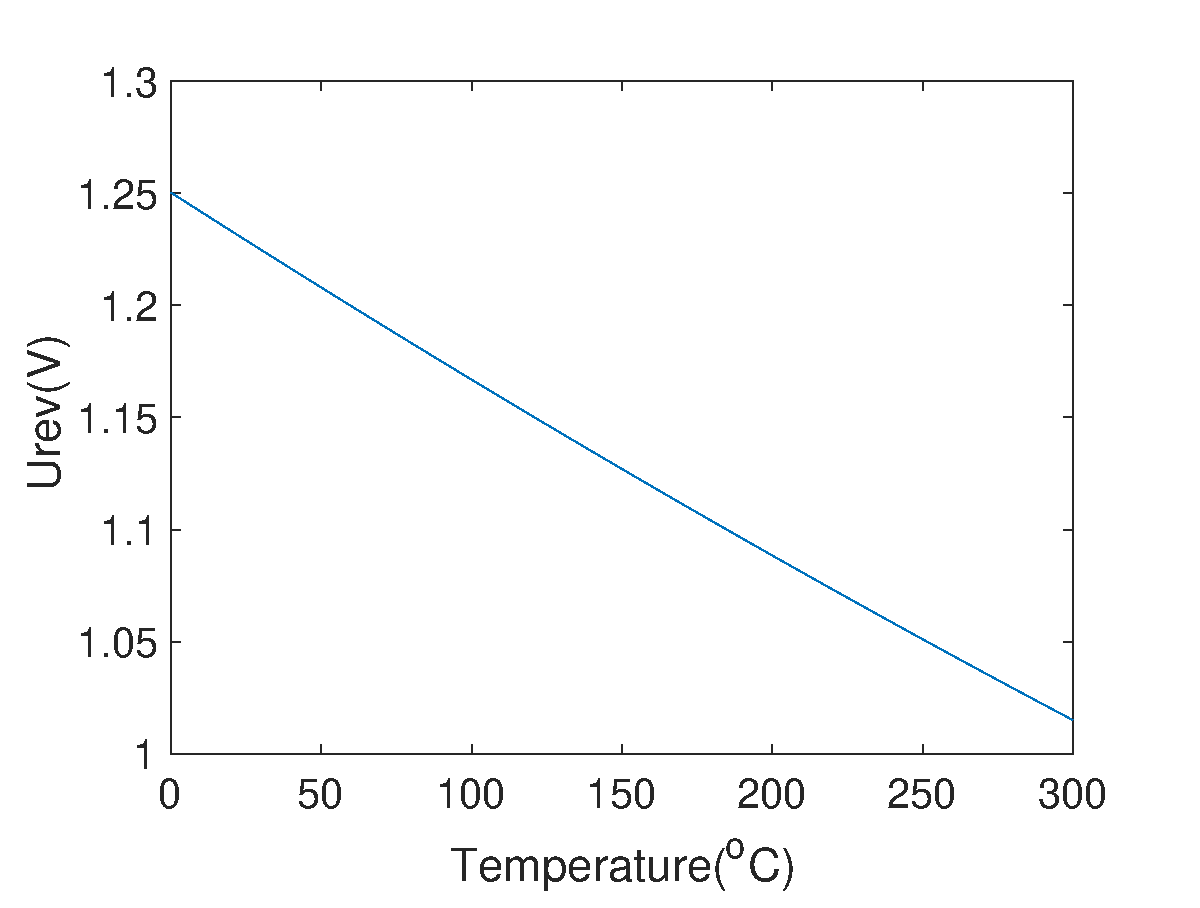
\includegraphics[width=5.5cm]{temperature.eps} 
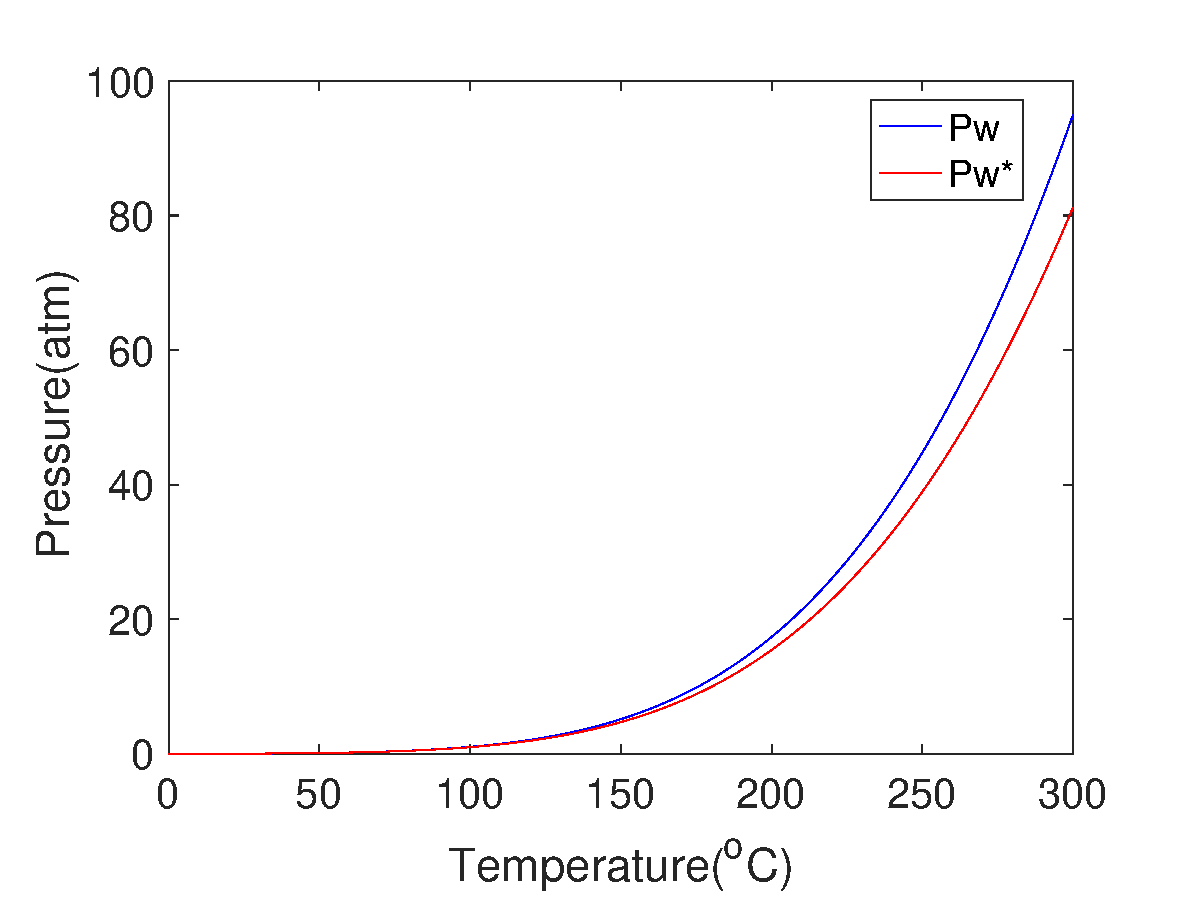
\includegraphics[width=5.5cm]{pw.eps} 
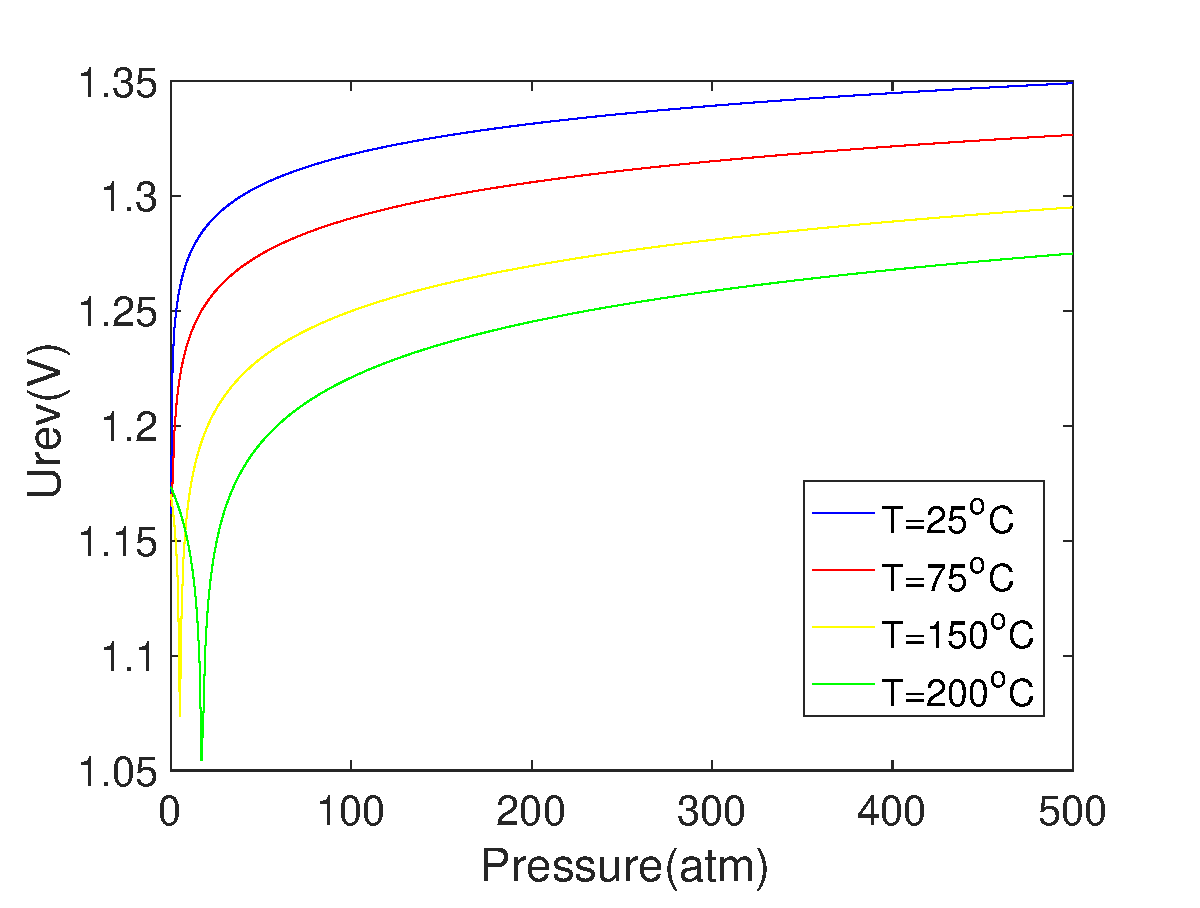
\includegraphics[width=5.6cm] {pressure.eps} 
\caption{a)Variation of reversible voltage with temperature; b)Pw and Pw* with temperature; c) pressure at various temperature, assuming 25\% concentration} 
\label{fig:Urev}
\end{figure} 
\subsubsection{Electrochemistry} 
The actual cell voltage would be higher than the reversible energy  as a result of irreversibility of the process. The cell voltage is the sum of reversible voltage, overpotential due to ohmic losses, activation overpotential and concentration overpotential.The concentration overpotential is small and therefore not considered in this model.
\begin{equation} 
U_{cell}=U_{rev}+U_{ohm}+U_{act}+U_{con}
\end{equation} 

%\begin{figure}[h]
%\centering
%\includegraphics[width=6cm]{electrochemical.png} 
%\caption{total cell voltage and reversible cell voltage}
%\end{figure} 

\subsubsection{Ohmic Overpotential} 
Each component in the electrolytic cell can be modelled as an electrical conductor. When current passes through the conductors, there is ohmic power loss due to the resistivity of the conductors which will lead to a heating effect. Since the electrolysis reaction is endothermic, some of the heat can be utilised within the system. While most ohmic energy is lost in the electrolytic solution, the membrane, wirings, electrodes  and bubble effects also form part of the electrical resistance. The heat generated can be evaluated by  $ Q=UI=I^2 R$, where R can be computed by:
 \begin{equation}
R=\frac{l} {A \kappa} 
\end{equation} 
where $ \kappa(S/m) $  is the conductivity of the solution.\newline
The total ohmic loss is the sum of all components in the electrolysis cell.
\begin{equation} 
R_{total}=R_{electric} + R_{anode}+ R_{cathode}+R_{bubble}+R_{ions} +R_{membrane} 
\end{equation} 
For the electrolytic solution, the area specific resistivity of the electrolyte can be calculated by:\cite{conductivity}
\begin{equation} 
r_{ions}=\frac{\delta_{el}} {\sigma_{el}(T,M) } 
\end{equation} 
where $\delta_{el}$ represents the electrolyte layer thickness and $\sigma_{el}$ represents the conductivity of the solution which varies with temperature and molarity.
The conductivity of electrolyte varies with temperature, concentration and composition. The specific conductivity of electrolyte (S/m) can be estimated by:\cite{conductivity}
\begin{equation} 
\sigma_{el} = (A(M) + B(M^2) + C(MT) + D(\frac{M} {T}) + E(M^3) +F(M^2T^2) )\times 100
\label{eq:sig}
\end{equation} 
where M represents the molarity in mol/L, and T is Temperature in Kelvin, and A-F are constants.
\begin{figure}[h] 
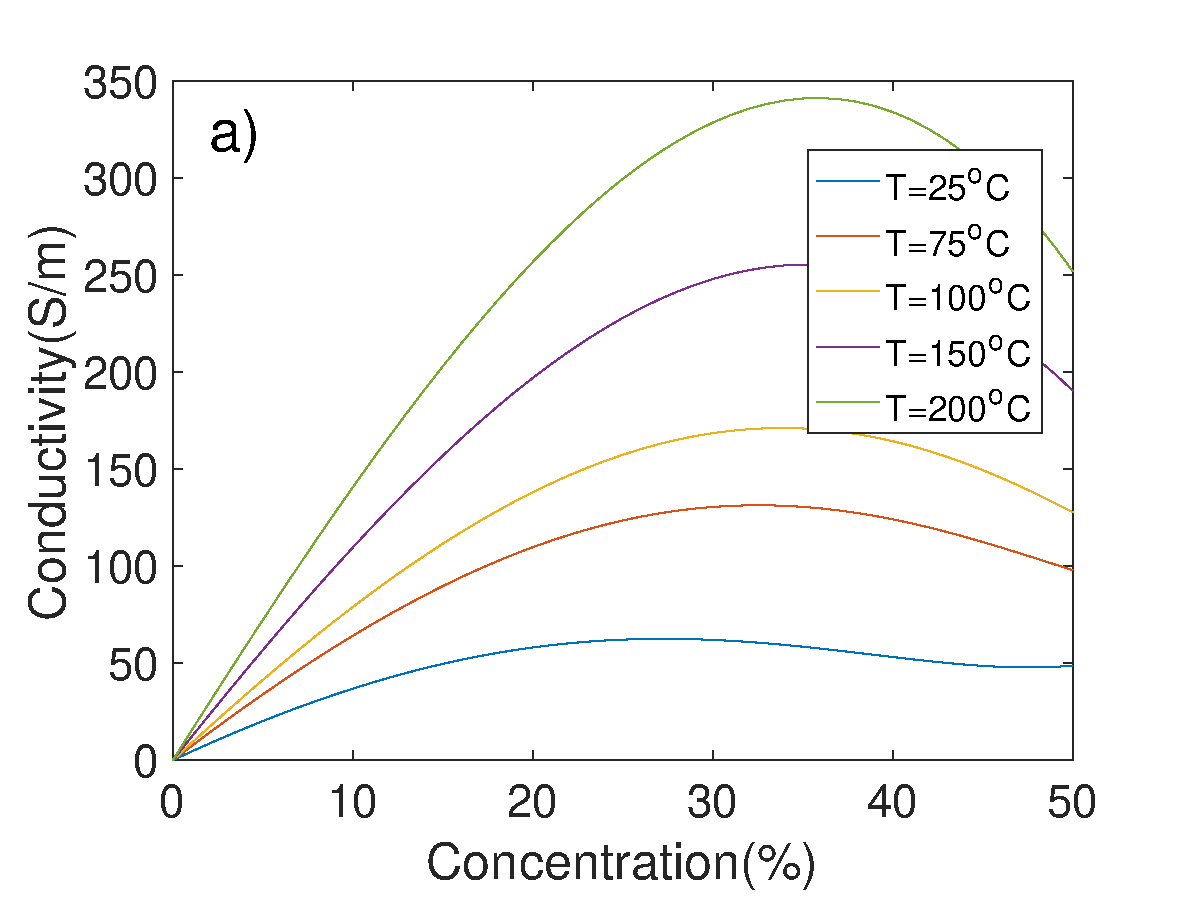
\includegraphics[width=5.5cm] {cond.eps} 
\includegraphics[width=5.5cm]{3D.eps}
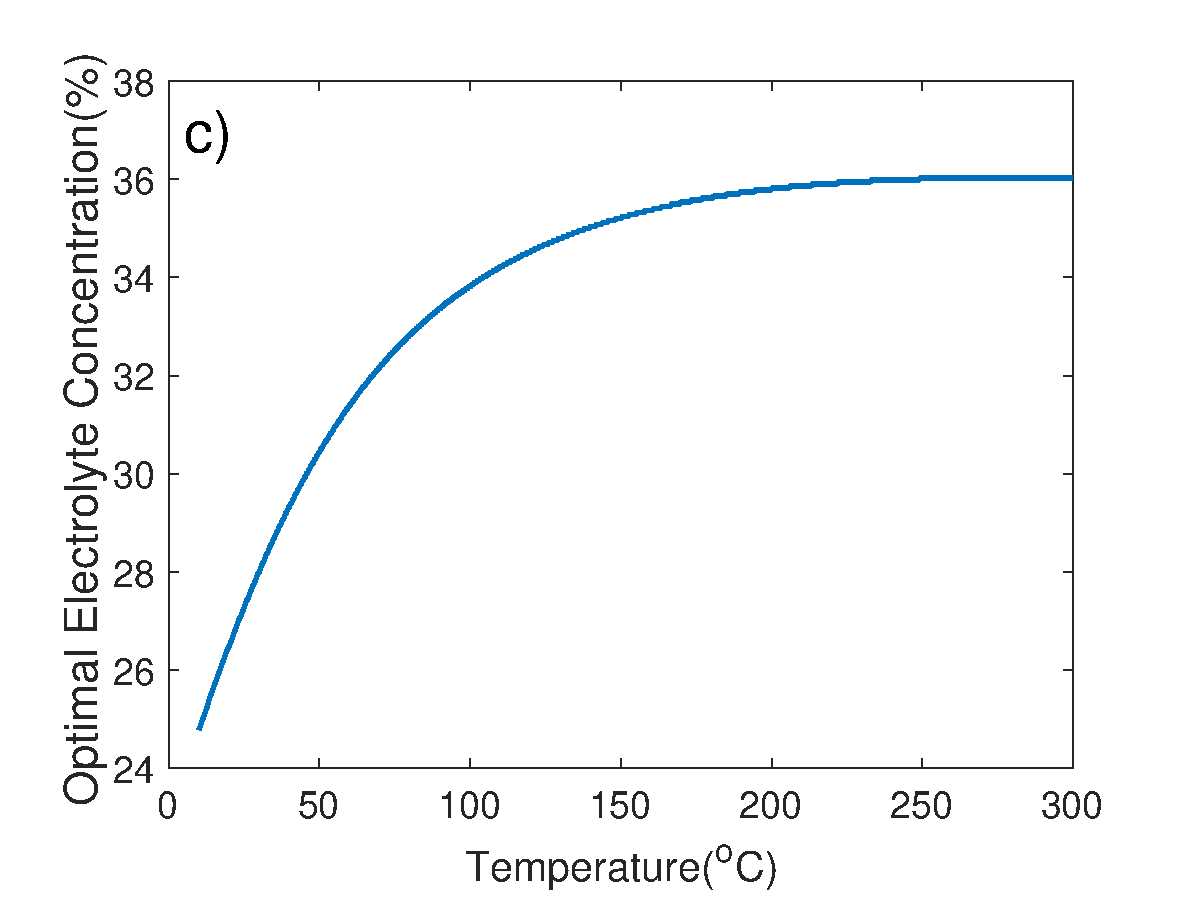
\includegraphics[width = 5.5cm]{optimum.eps}
\caption{ a)Variation of conductivity with temperature and concentration. b)3D plot. c) the optimal concentration of electrolyte with temperature} 
\label{fig:3D}
\end{figure} 
It can be seen from Figure \ref{fig:3D} that the conductivity increases when concentration is higher, this is due to the increase in the number of unit ions per volume in the solution. However the conductivity of the solution has a limit, and once that limit is reached, the conductivity starts decreasing with increasing concentration. It can also be shown that the conductivity increases with increasing temperature, because an increase in temperature may also cause an increase in the number of ions in solution due to dissociation of molecules. Also noteworthy is the existence of an optimal concentration which increases with increasing temperature: at above 200 degree Celsius, the optimal concentration reaches around 36\%. In reality, the electrolyte concentration is usually around 25 - 30 \% due to considerations on corrosion.
The ohmic overpotential from electrolytic solution is therefore:\
\begin{equation} 
U_{ohm} = r_{ions} \times J
\end{equation} 
where J is the superficial current density. 


%The conductivity is further decreased due to bubbles effects, The conductivity can be calculated using Bruggeman correction
%\begin{equation} 
%\sigma_B= \sigma_0(1-\alpha_{total} )^{1.5} 
%\end{equation} 
%where $\sigma_0$ is the conductivity with no bubbles and $\alpha_{total} $is the total void fraction.
 %overpotential is a specific form of concentration overpotential and is due to the evolution of gas at either the anode or cathode. This reduces the effective area for current and increases the local current density. The bubbles located on or very near to the elecuode surface contribute significant electrolyte conductivity loss because their population is very crowded at the gas evolving surface.

 %Which depends upon several factors including the rate of gas evolution at the electrode  $\frac{\dot{V_G}}{A}$ ,  the average residence time of bubbles at the electrode surface $t_r$, and the average bubble volume at departure from the electrode surface $V_r$.
%\begin{equation} 
%\Theta = \frac{\pi} {2} \frac{\dot{V_G}} {A} \frac{t_r}{V_r}{R_r} ^2
%\end{equation} 
%where $R_r$ is the bubble radius at detachment
%\begin{figure}[h] 
%\centering
%\includegraphics[width=10cm] {void} 
%\caption{Comparisons between experimental and modeling results } 
%\end{figure} 

%The electrode can be considered as a resistor in parallel with a capacitor, The space between the electrodes should be reduced to reduce the ohmic loss and to make the current density higher. For instant, the distance between electrodes is a typical example of less than 1 millimeter, known as a zero gap configuration method. Some manufactures commercial electrodes and membranes as the only components to make batteries, so that the real zero gap is achieved. \cite{zerogap}

%\begin{figure}[h] 
%\centering
%\includegraphics[width=10cm] {zerogapgap.png} 
%\caption{UI curve for different electrode distance \cite{zerogap} }
%\end{figure} 

\subsubsection{Resistance of the Membrane}
An empirical fitting of the resistance of the 0.5mm Zirfon based membrane and the temperature is presented as:\cite{activation4}
\begin{equation}
R_{mem} = \frac{0.06+80e^{T/50}}{10000S_m}
\end{equation}
where Sm is the membrane surface in $cm^2$.

\subsubsection{Activation Overpotential}
In reality, the efficiency of alkaline electrolysis is further reduced by electrode kinetics, making the actual electrode potential higher than the reversible potential. The difference is called the activation overpotential. This represents the kinetic barriers that need to be overcome for the gas evolution reactions at each electrode. Various experiments have shown that the overpotential for oxygen evolution reaction (OER) is much higher than for that the hydrogen evolution reaction (HER), and it depends heavily on the catalytic properties of electrode materials. \cite{activation} There are many other factors that influence the overpotential, including temperature, current density, concentration and impurity of the solution.
The corresponding current density can be calculated using the Butler-Volmer equation: \cite{activation1}
\begin{equation} 
J = J_0 [e(^{\frac{\alpha_a}{RT}zFU_{act,a}}) - e(^{\frac{\alpha_c}{RT}zFU_{act,c}})],
\end{equation}
where $J$ is the current density, $J_0$ is the exchange current density, which represents current at equilibrium, the oxidation and reduction reaction rates are opposite and equal, resulting in zero net current, and  $\alpha_{a/c}$ is the charge transfer coefficients. The charge transfer coefficients are related by temperature by:\cite{activation4}
\begin{equation} 
\alpha_a = 0.0675 + 0.00095T,   \alpha_c = 0.1175+0.00095T
\end{equation} 
For large overpotential, this can be approximated by the Tafel equation\cite{activation2} 
\begin{equation} 
U_{act,a/c} = 2.3026 \frac{RT}{zF\alpha_{a/c}} log(\frac{J}{J_0}).
\end{equation}
The exchange currents density is found experimentally, which can be significantly different depending on the electrode composition and temperature. The activation overpotential can be decreased by using catalysts, and this will be discussed later in the report. The activation overpotential at cathode and anode and the effects of temperature are shown in Figure \ref{fig:activation} . It can be shown that the activation overpotential increases with temperature, but this effect is quite small.
\begin{figure}[h] 
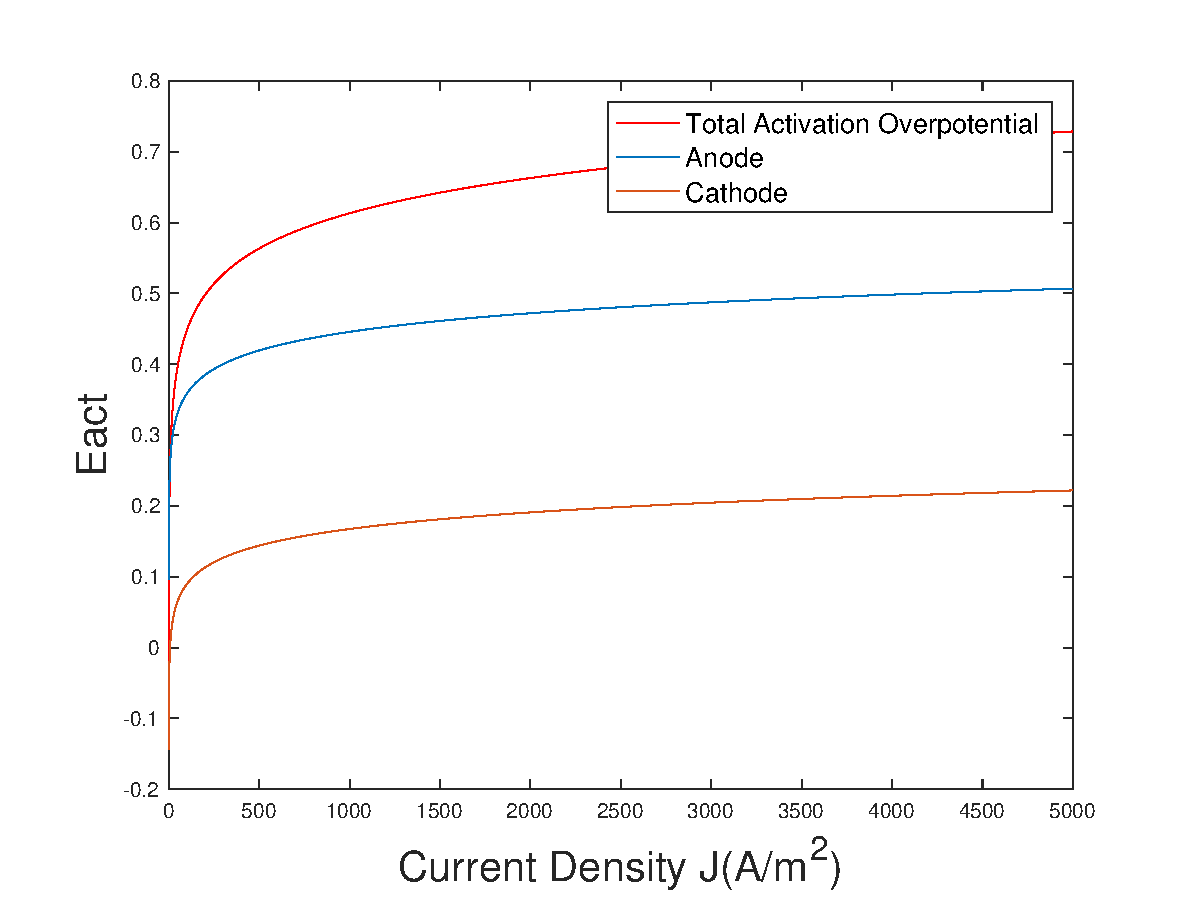
\includegraphics[width=8cm] {Activation.eps} 
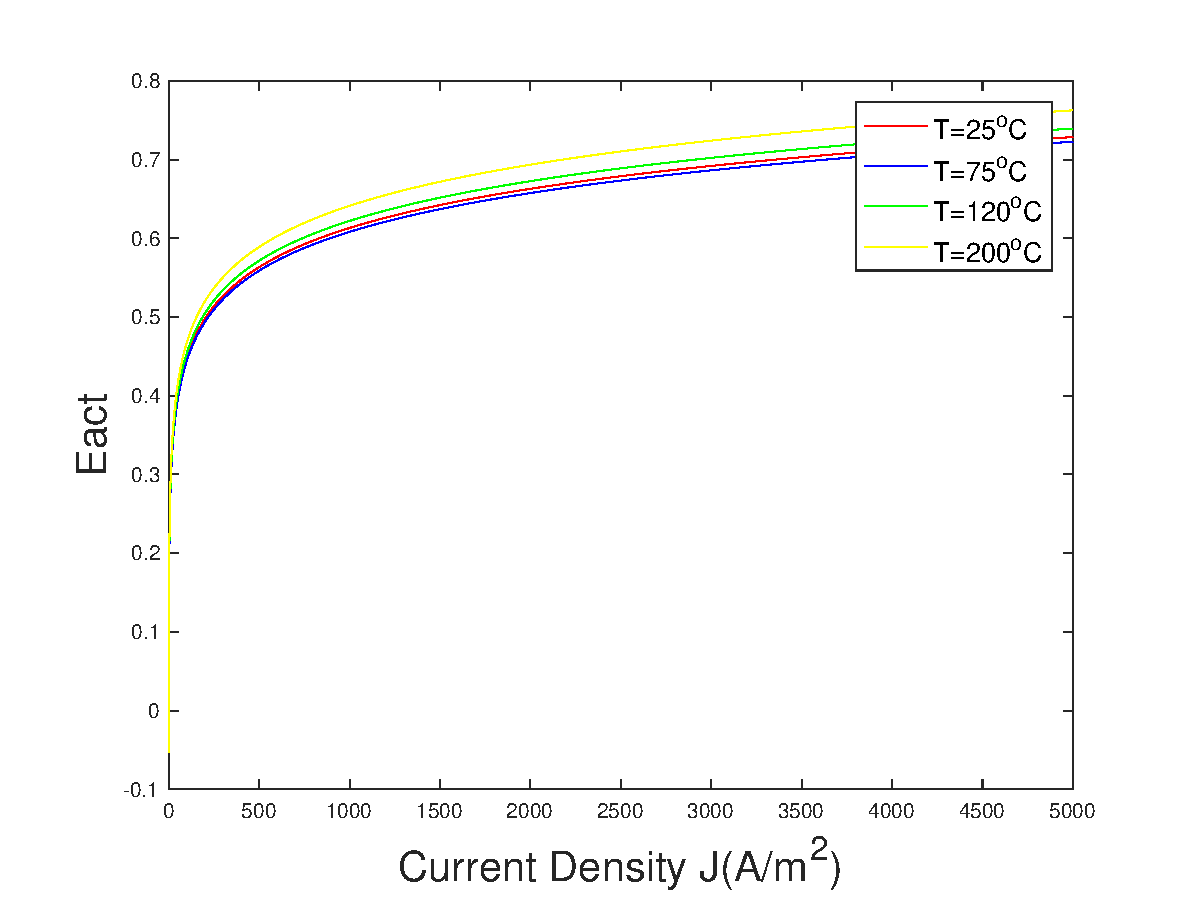
\includegraphics[width=8cm]{ActivationT.eps}
\caption{Activation Overpotential at cathode and anode(left),effects of temperature(right)} 
\label{fig:activation}
\end{figure} 

\subsubsection{Bubble Effects}
When hydrogen and oxygen are produced at the electrodes, bubbles will partially adhere to the electrodes, making a fraction of the surface electrochemically inactive so that current is applied to a smaller area. The effective surface area of the electrodes is:\cite{bubble2}
\begin{equation} 
S_{eff} = S(1-\theta)
\end{equation}
where $\theta$ is the bubble coverage ratio on electrode surface, with values between 0 and 1. As a result, the actual current density is greater than the superficial one, their relationship is:\cite{bubble2}
\begin{equation} 
Ja = \frac{J}{S_{eff}} = \frac{J}{1-\theta}
\end{equation} 
where $J_a$ is the actual current density, $J$ is the superficial current density, An empirical equation has been developed from experimental data that relates bubble coverage and superficial current density \cite{bubble2} 
\begin{equation}
\theta = 0.023(\frac{J}{Am^{-2}})^{0.3}
\end{equation} 
Apart from current density, the bubble coverage also depends upon several other factors such as the rate of gas evolution at the electrode surface.\cite{bubble2} The total activation potential combined with bubble effects can be calculated by\cite{activation4} 
\begin{equation} 
U_{act-\theta} = 2.3026\frac{RT}{zF\alpha_{a/c}}{log(\frac{J}{J_0}}) - 2.3026log(1-\theta) 
\end{equation} 
where the second term on the RHS represents the bubble effects. Another important effect of bubble formation is  the reduction of electrolyte conductivity, which will increase the ohmic resistance of the electrolyte. The effective conductivity  can be calculated using the Bruggman equation:\cite{void} 
\begin{equation}
\sigma_B = \sigma_0(1- \alpha_{total})^{1.5}
\end{equation}
where $\alpha_{total}$ is the void fraction, which is the fraction of volume occupied by the gas. $\sigma_0$ is the conductivity without any bubbles and $\alpha_{total}$ is the total void fraction. Unlike many other models  that were developed from assuming equal-sized spheres, the Bruggman model was derived assuming many different bubble sizes.  As can be seen from Figure \ref{fig:what}c), the conductivity reduces rapidly with increasing void fraction. When temperature $= 120^oC$ for example, a void fraction of 0.37 halves the conductivity. %The voltage loss as a result of conductivity reduction can be calculated by\cite{void2}
%\begin{equation}
%V_{ohm} = \frac{\delta_{el} J_{av}}{\sigma_B}
%\end{equation}
%where $J_{av}$ is the average current density, and $\delta_{el}$ is the electrolyte layer thickness.
The void fraction is related by bubble coverage by\cite{activation2}
\begin{equation}
\alpha_{total} = \frac{2}{3}\theta
\end{equation}

\begin{figure}[h] 
\centering
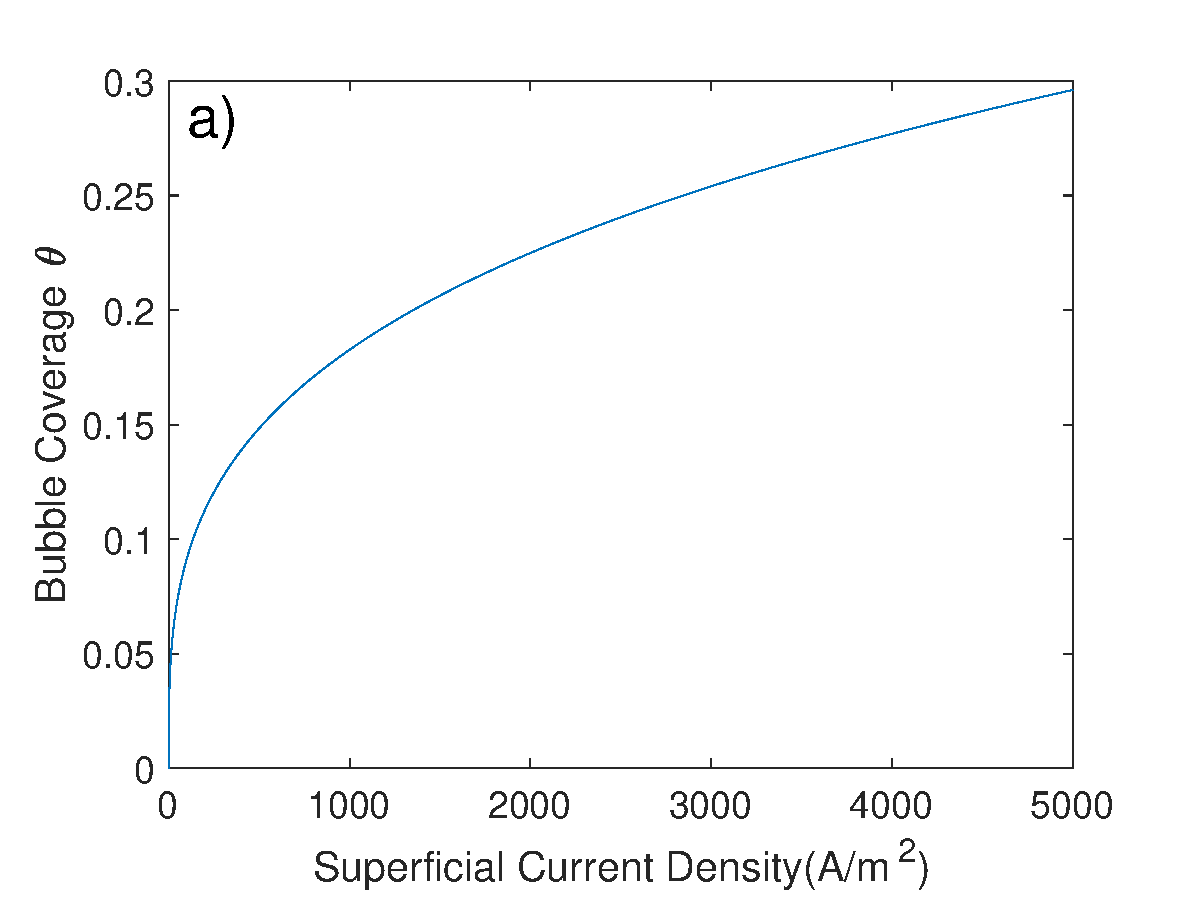
\includegraphics[width=7cm]{coverage.eps}
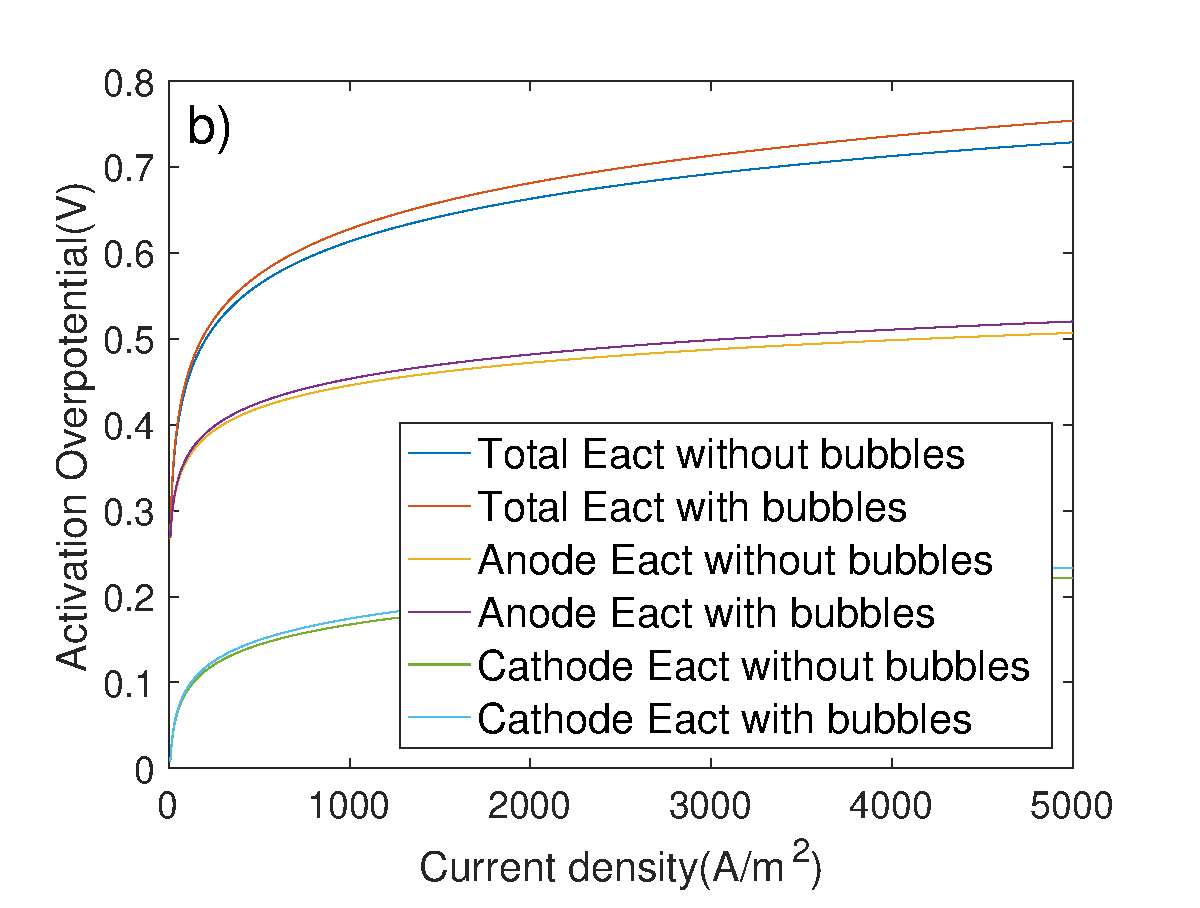
\includegraphics[width=7cm] {actbubble.eps} 
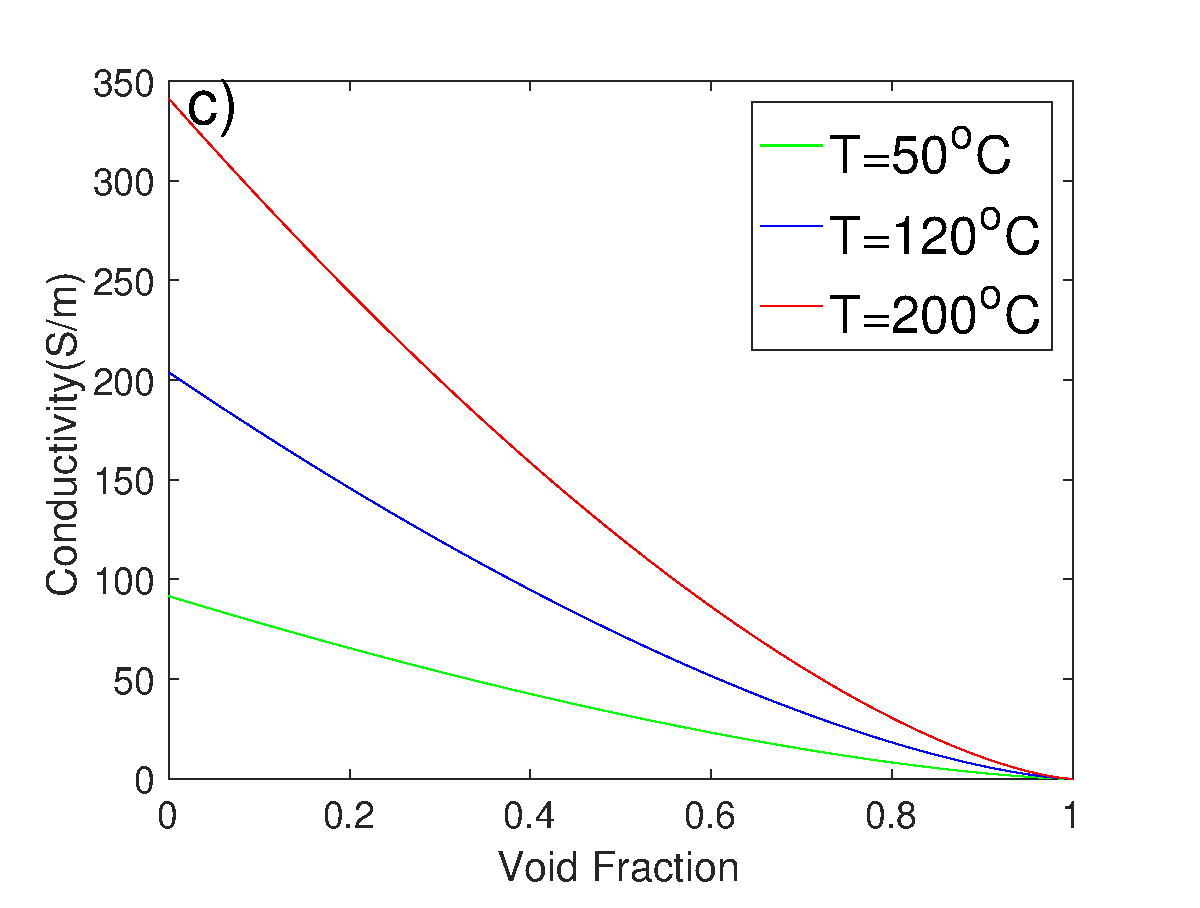
\includegraphics[width=7cm]{void2.eps}
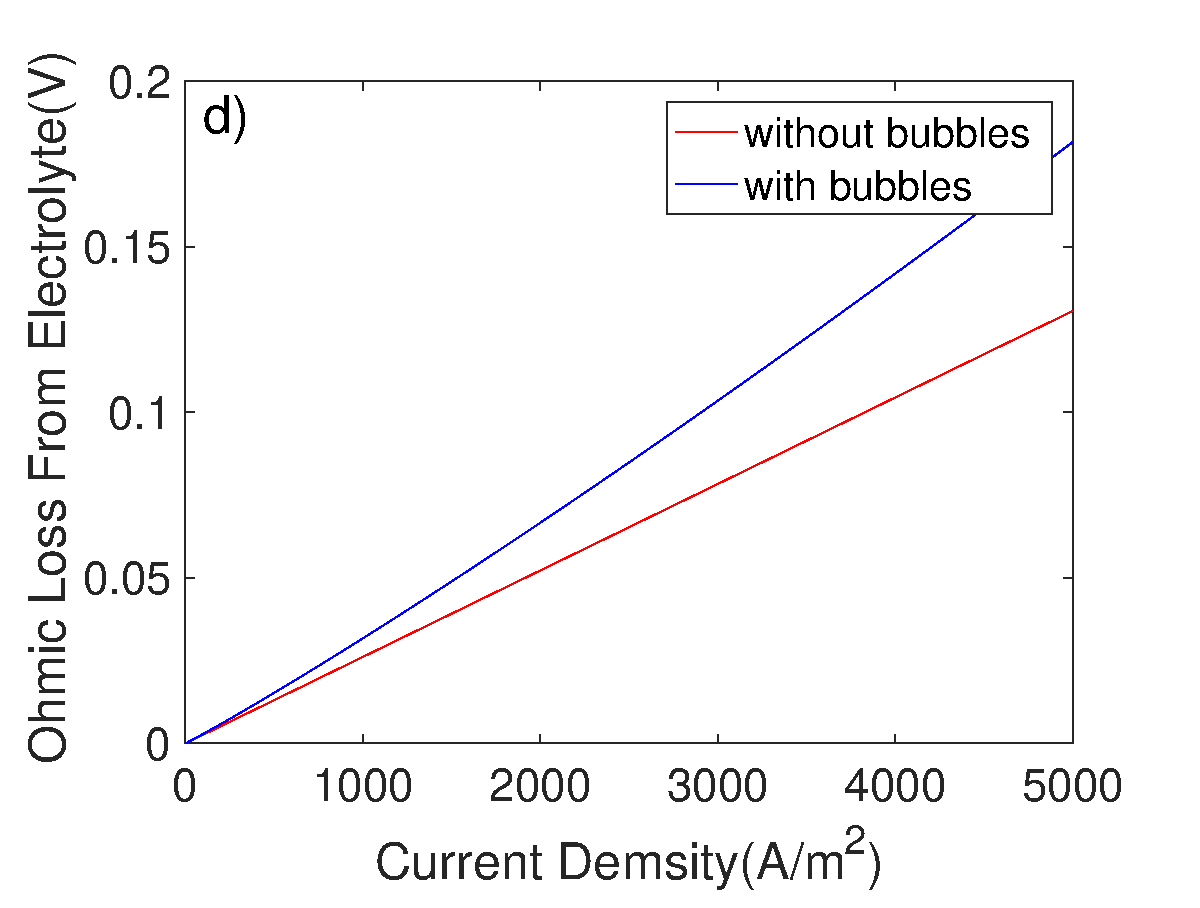
\includegraphics[width=7cm]{bubble3.eps}
\caption{a)Bubble coverage against current density. b) Activation Overpotential taking into account the bubble effects at electrodes against current density. c)Conductivity against void fraction d) Ohmic voltage loss from electrolyte with and without bubbles} 
\label{fig:what}
\end{figure} 



\subsubsection{Overall Cell Voltage and Optimum Operating Conditions}
The polarisation curve of the alkaline electrolysis cell is plotted in Figure \ref{fig:ni}a), it is observable that the total cell voltage increases with higher current density. This is largely due to the increased contribution from ohmic losses, especially from bubble formation, whereas the curve for activation polarisation actually becomes flatter at higher current density. This means that a lower current density will lower the energy consumption and thus increase the system efficiency. However, the hydrogen production rate, which increases with higher current density,  is also an important factor to consider along with the system efficiency.  Electrolyser degradation and safety issues also influence the choice of current density. The rate of electrolyser degradation increases rapidly with higher current density and this will thus increase the investment cost. The large amount of heat produced as a result of higher current density, if poorly managed, can be dangerous. In addition, gas crossover is more significant at low current density, and this is because although the amount of gases crossing over the membrane remains the same, there are smaller amounts of gases produced to dilute the effects. The result is a highly flammable mixture once it reaches a certain limit. In industry, a compromise has to be made. The current density is usually kept between 1000 - 3000$A/m^2$. \cite{currentdensity}

\begin{figure}[h]
\centering
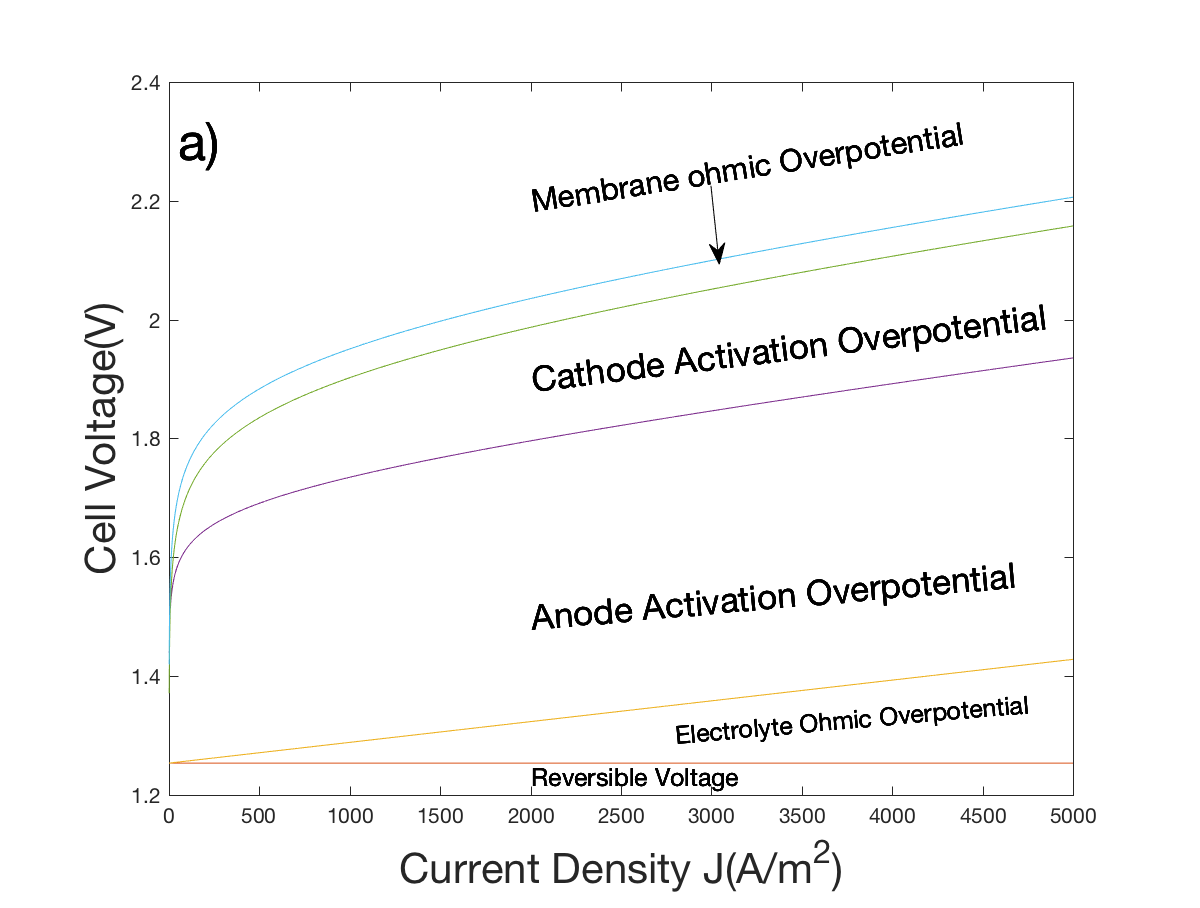
\includegraphics[width=9cm]{total.eps}
\newline
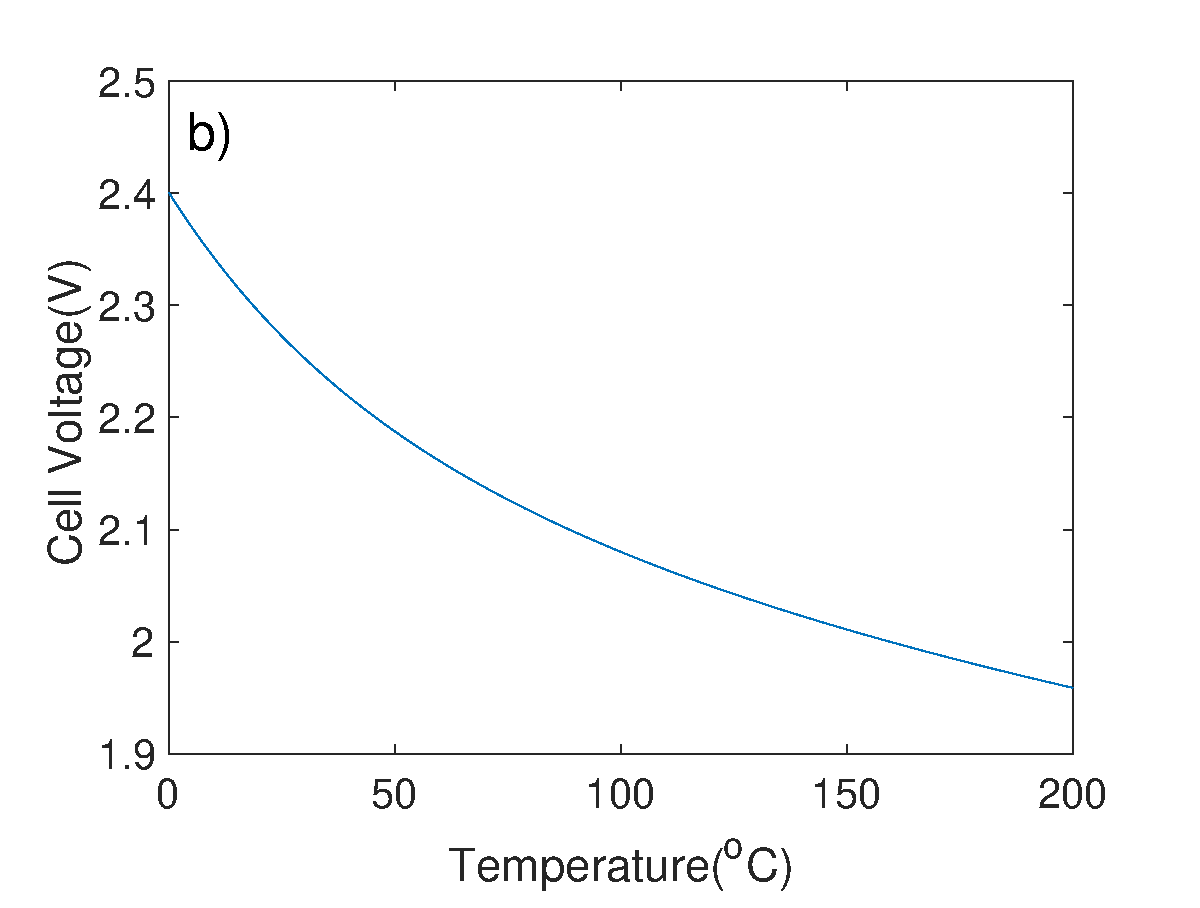
\includegraphics[width=7cm]{cellT.eps}
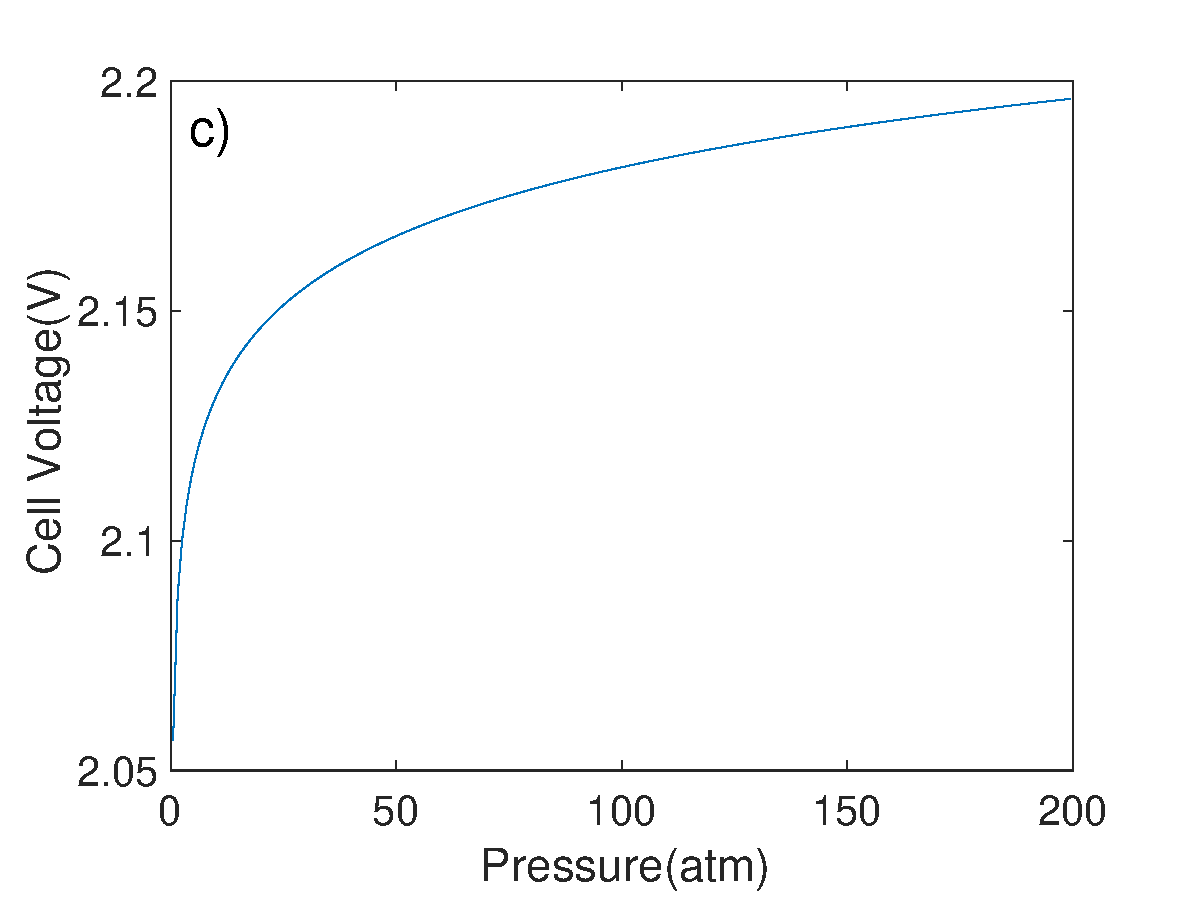
\includegraphics[width=7cm]{cellP.eps}
\caption{a)Total cell voltage showing cumulative effects of reversible voltage, activation and ohmic overpotential. b)Total cell voltage against temperature. c)Total cell voltage against pressure}
\label{fig:ni}
\end{figure}
Raising the operating temperature is one of the most effective ways to improve efficiency. As can be seen in Figure \ref{fig:ni} b), increasing the operating temperature reduces the cell voltage, as a result of decreased reversible voltage, higher ionic conductivity, and lower activation overpotential due to enhanced electrode surface kinetics. However, a high temperature can lead to high corrosion risk which will require more expensive materials. Also, the water loss from evaporation increases with higher temperature. Conventional electrolysis system is operated around 80 - 90$^oC$, just below the boiling point of water.\cite{temp} There are two major ways to further elevate the operating temperature, the first way is to use a pressurised system which will increase the boiling point of electrolyte, and in industry this is usually kept at 120-150$^oC$.\cite{temp} The second way is to carry out steam electrolysis which can increase the temperature even further to a level of above 500$^oC^$.\cite{temp} However this method has not become commercialized in industry due to its high economic cost. \\
Pressure is another very important parameter, increasing operating pressure has several positive effects apart from allowing for higher operating temperature.  A high pressure would reduce the size of bubbles, and gases increase in solubility with increased pressure. This will reduce the ohmic loss from bubble formation. Obtaining pressurised hydrogen is also more energy efficient during the compression process. Also, higher operating pressure makes the process of hydrogen drying easier. However, at high pressure, there is more gas crossover due to diffusion since the partial pressure of both gases have increased. A high pressure also slightly increases the operating cell voltage. In industry, 
hydrogen production at a pressure of up to 30 bar is  commercial available, and this can be achieved by using a feed-water pump.\cite{gibbs}


\subsubsection{Electrolyser Efficiency }  
Efficiency is one of the key design objectives for the electrolysis system. There are three main efficiencies to consider depending on how the system is assessed.\cite{currentdensity} The voltage efficiency is the proportion of effective voltage for water decomposition to the overall cell voltage and presents as:
\begin{equation}
\eta_{voltaic} = \frac{E_{anode} - E_{cath} }{U_c}
\end{equation}
A more commonly used expression is the Faradic efficiency, which relates the reversible voltage to the overall cell voltage, it also represents the percentage of the actual to theoretical hydrogen production. Its value is usually lower than 1 which means that there exist the consumption of energy that does not contribute to the hydrogen production due to the parasitic currents in the system. \cite{currentdensity}
\begin{equation}
\eta_{Faradic} = \frac{\Delta G}{zFU_c} = \frac{U{rev}}{U_c} 
\end{equation}
The thermal efficiency takes into account the thermal energy and can be calculated by
\begin{equation}
\eta_{Thermal} = \frac{\Delta H_{t,p}}{zFU_c} = \frac{U_{th}}{U_c} 
\end{equation} 
where $\Delta H_{t,p}$ is the enthalpy change of water decomposition. The thermal efficiency is 100\% if the cell voltage is equal to the thermoneutral voltage. When cell voltage is higher than $U_{th}$, the efficiency is lower than 100\%, and the process is exothermic. A thermal efficiency of over 100\%, which is when the cell voltage is below the thermoneutral voltage,  is theoretically achievable in high temperature steam electrolysis but is generally unpractical for alkaline electrolysis system. Under standard conditions, $U_{rev} = 1.23V$ and $U_{th} = 1.48V$. The relationship between $U_{rev}$ and $U_{th}$ against current density is plotted in Figure\ref{fig:my} a).
\begin{figure}[H]
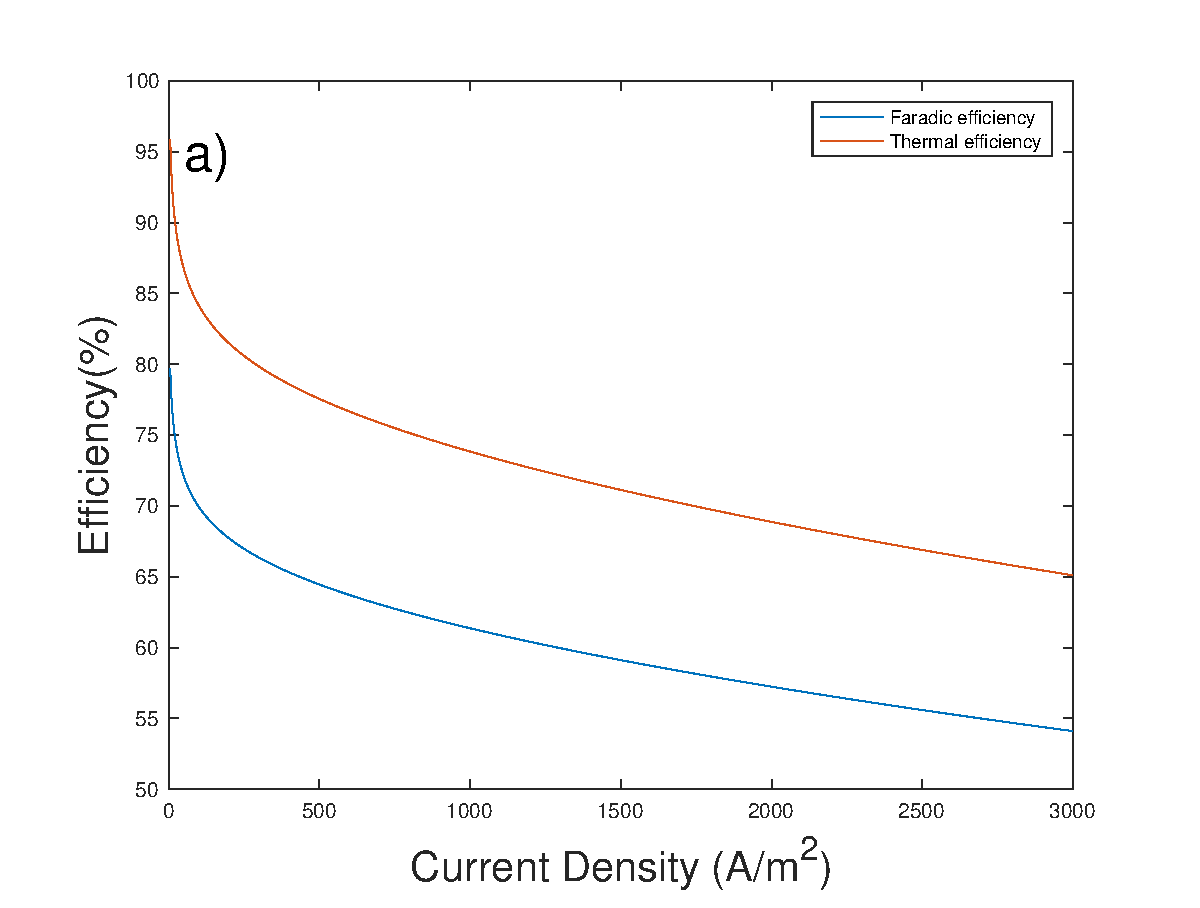
\includegraphics[width=8cm]{efficiency.eps} 
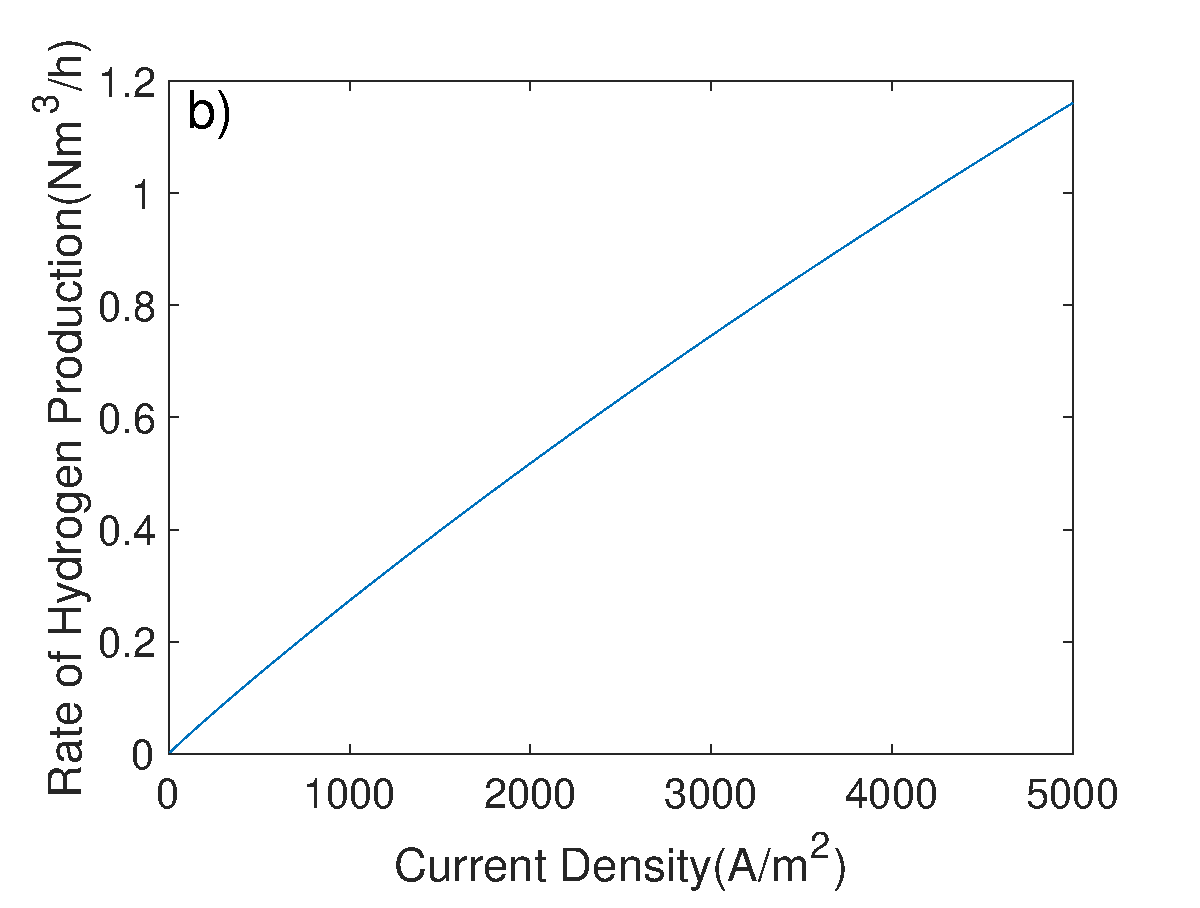
\includegraphics[width=8cm]{rate.eps}
\caption{a)Comparison of Faradic and Thermal efficiency. b)Hydrogen production rate (single cell)}
\label{fig:my}
\end{figure} 

As discussed before, a compromise has to be made between efficiency and hydrogen production rate, which is shown in Figure \ref{fig:my} b).

%\begin{equation} 
 %f_{H2} = \eta_F %\frac{N_{cell}I_{cell}}{zF}\frac{22.41}{1000}3600
%\end{equation} 
Another important parameter for the electrolysis process is the specific energy consumption,which can be calculated for a given time interval t as:\cite{efficiency2}
\begin{equation}
C_E = \frac{\int_{0}^{t} N_{cell}  {I_{cell}}  V_{cell} dt}{\int_{0}^{t} f_{H2}dt}
\end{equation}

Finally, the electrolyser efficiency or the HHV efficiency can be calculated using the specific energy consumption by:\cite{efficiency2}
\begin{equation}
\eta_E = \frac{HHV of Hydrogen}{C_E} 
\end{equation}
where HHV is the higher-heating-value of hydrogen. It assumes that the energy absorbed by water can be released and reused in the system by converting water back to its initial standard conditions. However, recovering the full higher-heating value is not practical in reality.
The electrical-energy efficiency can be calculated using the higher-heating voltage.\cite{efficiency} \cite{efficiency2} 
\begin{equation}
\eta_E=\frac{V_{HHV}}{V_{cell}}
\end{equation}

\begin{figure}[H]
\centering
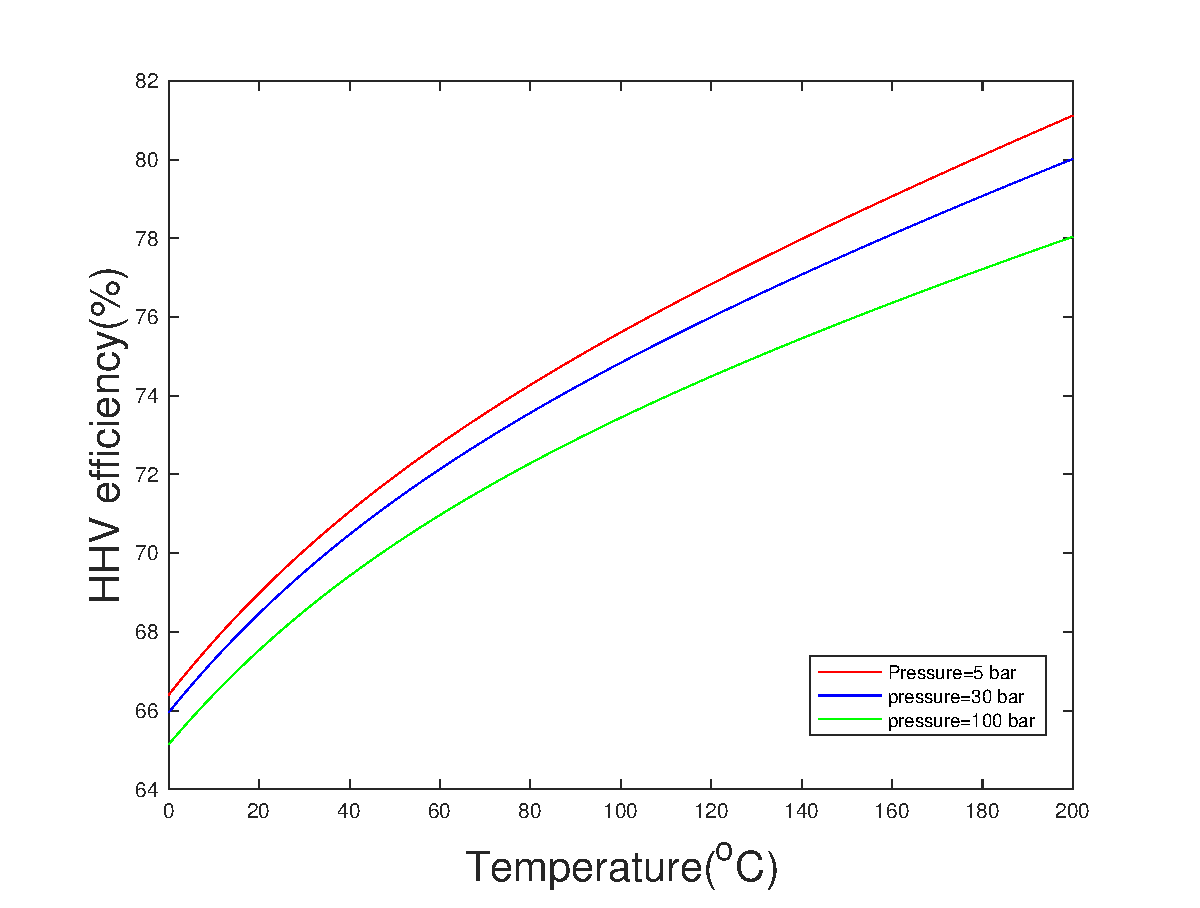
\includegraphics[width=8cm]{HHV.eps}
\caption{Variation of HHV efficiency against temperature at different pressure}
\label{fig:HHV}
\end{figure} 
The HHV efficiency at different temperatures and pressures with fixed current density is shown in Figure \ref{fig:HHV}, It can be seen that the efficiency increases with increasing temperature and decreases with pressure. A summary of operating conditions and key parameters are shown in Table \ref{tab:oo}.

\begin{table}
\centering
\begin{tabular}{ |c|c| } 
 \hline
 Temperature & $120 - 150 ^oC$  \\ 
 \hline
 Cell area & $1m^2$\\
 \hline
 Pressure & 30 bar \\
 \hline
 Membrane thickness & 0.5mm\\ 
 \hline
 Electrode thickness & 2cm\\
 \hline
 Electrode height & 45cm\\
 \hline
 Electrolyte and Concentration & KOH $30\%$\\
 \hline
 Minimum/Maximum current density & 1500/5000 $A/m^2$\\
 \hline
 Minimum/Maximum Cell voltage & 1.98/2.25V \\ 
 \hline
 $\eta_F$ at Minimum/Maximum load & 62\%/ 56\% \\ 

 \hline
 $\eta_{Thermal}$at Minimum/Maximum load & 75\%/67\% \\ 
 \hline
 HHV efficiency at Minimum/Maximum load &  76\%/68\% \\ 
 \hline
 Minimum/Maximum Flow rate(per cell) & 0.0048$mols^{-1}$/0.0145$mols^{-1}$\\
 \hline
\end{tabular}
\caption{\label{tab:oo}Operating conditions and key parameters.}
\end{table}




%From Faraday?s law, the hydrogen production rate is proportional to the current I which represents the charge transfer in an electrolysis cell, Assuming that the same current flows through every electrolyzer cell, the hydrogen production rate in Nm3/h can be expressed as
%\begin{equation} 
%f = \eta_F \frac {NI} {zF} 
%\end{equation} 
%Where N the number of cells, I the current of cell, $\eta_F$ is the Faraday efficiency which represents the percentage of the actual production to theoretical production, its value is usually lower than 1 which means there exists the consumption of the energy that does not contribute to the hydrogen production.The maximum value of the Faraday efficiency is usually above 0.95A. Also, the electrolyser efficiency $\eta_E$ should be taken into account. It can be calculated as the ratio betwwen HHV of hydrogen and energy consumption.


\subsection{Electrolyser Design} 
%\subsubsection{Wind Power Generation System} 
 %The configuration of the wind power generation sys-tem considered in this study is shown  below:
%In order to get the Maximum Power, the system will use wind turbine's Maximum Power Point Tracking method. MPPT is a fully electronic system that varies the electrical operating point of the modules so that the modules are able to deliver maximum available power. Power captured from wind can be calculated using
%\begin{equation} 


\subsubsection{Configuration} 
Currently there are two types of electrolyser configuration: unipolar and bipolar, which is shown in Figure \ref{fig:con}. In a unipolar configuration (or tank-type), the electrodes with the same polarity are connected in parallel, therefore the total cell voltage is the same as the voltages of individual cells, and the total current is the sum of currents in each cell. A bipolar electrolyser usually has a larger number of cells with the electrodes connected in series, and the electrodes each have both the positive and negative polarities. So current is the same in each cell and at the terminals. Unipolar electrolysers operate at a low voltage level of 1.9 - 2.5 V,\cite{configuration} but they require a high level of current. On the other hand, bipolar configuration requires a low current but a voltage of $V_{cell} \times (n-1)$, which is about 35-600V.\cite{configuration} $V_{cell}$ is the voltage for each cell and n is the number of electrodes. The industrial electrolysers are mostly bipolar electrolysers.
The pros and cons of each type of configuration are shown in Table \ref{tab:ooo}.

%The compact structure of the bipolar electrolyzer reduces the loss caused by the resistance of the electrolyte, thus improving the efficiency of the electrolyzer. But on the other hand, the bipolar electrolyzer has increased the complexity of design because of its compact structure, resulting in the manufacturing cost higher than that of the monopole electrolyzer. In view of the current emphasis on conversion efficiency, the industrial electrolyzer is mostly bipolar electrolyzer.

\begin{figure}[H] 
\centering
\includegraphics[width=7cm] {monopolar.png} 
\includegraphics[width=7cm] {bipolar.png} 
\caption{Electrolyser configuration a)Monopolar configuration; b)Bipolar configuration.\cite{configuration}} 
\label{fig:con}
\end{figure} 
\begin{singlespace}
\begin{table}
\begin{tabular}{|p{7.9cm}<{\centering}|p{8.6cm}<{\centering}|}
 \hline
 \textbf{Unipolar} & \textbf{Bipolar} \\ 
 \hline
 \multicolumn{2}{ | c |}{\textbf{Advantages}} \\

 \hline
 Simple design and therefore easy to fabricate & The compact structure reduces electrolyte ohmic loss, thus improves efficiency \\
 \hline
Do not have parasitic currents & Operate at higher temperature and pressure \\
 \hline
 Cells can be individually isolated and carry out maintenance & Operate at higher current density which increases rate of production\\
 \hline
 Low maintenance requiremnet & Small requirement in space\\
 \hline
  \multicolumn{2}{ | c |}{\textbf{Disadvantages}} \\
  \hline 
Large Ohmic losses due to high currents and low voltages &  Parasitic currents which cause efficiency loss and corrosion problems\\
   \hline 
Large space required & High requirements in precision and complex system design\\
\hline
 Large limitation in raising operating temperature and pressure & Production needs to be stopped for maintenance\\
 \hline
 Difficult to achieve small interelectrode gaps & Requirement for electrolyte circulation\\
 \hline
 Heavy intercell busbars & Requirement for external gas/electrolyte separator\\
 \hline
\end{tabular}
\caption{\label{tab:ooo}Pros and cons of monopolar and Bipolar configuration.\cite{configuration2} \cite{efficiency2} }
\end{table}
 \end{singlespace}
\subsubsection{Cell Geometry} 
Apart from adjusting the operating conditions, proper choice of cell geometry is another way to improve performance. Some of the key design parameters include size of inter-electrode gap, height and inclination of electrodes. The smaller the gap between the electrodes, the smaller the volume of the electrolyte and thus the lower the ohmic overpotential. However, in the conventional configuration, reducing the inter-electrode gap could increase the contribution of cell resistance from gas bubbles, making the optimal gap to be larger than 2mm. This problem can be solved by adopting zero-gap configuration.\cite{zerogap}A series of experiments\cite{geometry} were conducted to identify the effects of electrode height and inclination, and it has been found that although selecting larger electrodes will enlarge the surface area and thus the current path, when the current density is large, higher efficiency can be achieved using smaller electrodes. This is 
because bubbles tend to accumulate at higher parts of the cell, increasing the void fraction. The experiments also showed that placing the electrodes at perfectly vertical position reduces the ohmic overpotential. 
\subsubsubsection{Zero-gap Configuration}
The zero gap cell involves two porous electrodes that are compressed and in contact with the membrane (Figure\ref{fig:Data1}), making the inter-electrode gap the same as the thickness of the membrane( $<$  0.5 mm).\cite{zerogap}The bubbles are released from the rear of the electrodes, which also reduces the contribution of cell resistance from the gas bubbles. Between the porous electrode and the bipolar plate is the gas diffusion layer, which not only provides an electrical connection, but also allows the feed of the electrolyte and the release of oxygen and hydrogen.This configuration can be assembled by depositing a catalyst layer onto the electrode, and then compressed onto the membrane, and finally gaskets are assembled to avoid leaking.The disadvantage of this configuration is the increased potential for the gas bubbles to block the electrode-membrane interface.
\begin{figure}[H] 
\centering
\includegraphics[width=6cm]{zerogap.png}
\caption{Zero-gap and non zero-gap configuration  }
\label{fig:Data1}
\end{figure}

%\subsubsubsection{Membrane-less Electrolyser}
%In a conventional electrolyser, a membrane is used to separate the oxygen and hydrogen gases. However, membranes can be expensive to produce and may not be stable. Membraneless electrolysers have been developed to solve the problem. Figure 15 shows the principle of membraneless Divergent Electrode-Flow-Through (DEFT) alkaline electrolyser. The technology is based on the parallel arrangement of porous electrodes which are separated by an electrode gap.The liquid electrolyte is first introduced into the high pressure distribution chamber, and then the fluid is subsequently introduced into the gap between each electrode. Instead of using a membrane to separate the oxygen and hydrogen gases, the gases are separated by fluid mechanic forces.\cite{membraneless2} One of the biggest advantages of this design is that there are almost no gas bubbles forming between the electrodes, thus have the potential to operate at a higher current density than the conventional electrolyser. An appropriate electrolyte flow velocity is required to reduce the gas bubbles to a negligible volume, and also prevent gas contamination to ensure a high hydrogen purity. Using the membraneless DEFT technology, a hydrogen purity of 99.83\% can be achieved with an electrode gap of 2.5mm and a minimum velocity of 0.075m/s.



\subsubsection{Electrode Material} 
The anode material must have good conductivity, high catalytic activity, good mechanical stability, resistance to electrolyte corrosion, in addition to an acceptable cost. Currently, the most commonly used anode is nickel or nickel based alloy. Nickel has good corrosion resistance compared with stainless steel or iron electrode and low price in alkaline medium. At the same time, nickel has high oxygen evolution potential and high oxygen evolution efficiency. One way to improve efficiency is to increase the electrode surface area in order to reduce the real current density and thus the activation overpotential. For example, a porous anode can be developed by sintering nickel powders, it has been shown that the porous high-surface area anodes have lower oxygen evolution overpotential than smooth anodes under elevated temperature and pressure (30 bars, 200$^oC$). Sintered, porous nickel coating is an another way to reduce overpotential which involves a lower sintering temperature. It has also been shown that an increase in coating thickness will raise the exchange current density and reduce the overpotential. Comparable effects in overpotential reduction can be achieved by using Raney alloys such as Raney nickel, Raney cobalt or Raney nickel-cobalt which will be covered with Ni or Co oxides during electrolysis.\cite{anode} \cite{anode2}


The cathode materials for hydrogen production in early age were mainly Pt, Pd and its alloys. Although these alloys have very low hydrogen evolution overpotential, they are expensive and can not be widely used to popularise.  So industry prefers inexpensive, low hydrogen overpotential alternatives such as Raney nickel or nickel based alloys like NiMo, NiSe and $NiS_2$. For cathode, the electrocatalyst's behaviours depend on its ability to adsorb hydrogen atoms, which is related to the strength of the metal hydrogen bond (M-H). \cite{cathode2}A stronger M-H bond would reduce the HER activation energy. However, if the adsorption energy is too high, the desorption of hydrogen becomes difficult. Therefore, a suitable M-H bond strength is required for the cathode. It can be seen from Figure \ref{fig:ca} that Pt has the highest activity, and Ni also have suitable bond strength while being inexpensive at the same time.  Zhang et al.\cite{cathode} compared the electrocatalytic activities of several nickel-based alloys (Ti/NiM where M represents different metals and Ni foil is the substrate). It can be shown from Figure \ref{fig:cat} that Ti/NiPt electrode has the highest catalytic activity, and they are all relatively stable. Ti/NiCo is the most suitable choice when electrolytic activity, stability and cost are all taking into account. In this model, Raney nickel anode and Ti/NiPt cathode are adopted.
\begin{figure}[H] 
\centering
\includegraphics[width=6cm]{catalyst.png}
\caption{Electrocatalytic activity against M-H bond strengh\cite{cathode2}}
\label{fig:ca}
\end{figure}
 
\begin{figure}[H] 
\centering
\includegraphics[width=6.1cm]{polarization.png}
\includegraphics[width=6.1cm]{stability.png}
\caption{Polarization curve for Ti/NiM electrode(left); Long term stability of catalytic Ti/NiM electrode for HER recorded at 1V(right)
\label{fig:cat}
\cite{cathode}}
\end{figure}


\subsubsection{Electrolyte and Ionic Activator}
The selection criteria for the electrolyte include: high ionic conductivity;  does not decompose chemically under supplying voltage; lower volatility so is not removed with the product gas. Alkaline electrolyte is adopted instead of acid electrolyte because the alkaline electrolytes have less issues with corrosion. KOH and NaOH solutions are common electrolyte choices, and KOH solution has higher specific conductivity than NaOH and is therefore used in this model. Although re-circulation of electrolyte is designed, there will be some electrolyte loss in reality through gases. It is therefore necessary to adjust the amount of electrolyte in the cell. 
%\begin{figure}[H]
%\centering
%\includegraphics[width=8cm]{electrolytematerial.png}
%\end{figure}
The energy consumption can be further reduced by the addition of an ionic activator. Lj et al. \cite{ionic} investigated the effect of adding an Novel ternary Ni $-$ Co $-$ Mo based ionic activator to the alkaline KOH solution. It has been found that the electrolyzer with in-situ activated electrolyte has an efficiency about 15\% higher than the standard KOH solution, and an energy consumption saving of about 17\%. The energy saving is proved to be more efficient at higher temperatures and current densities. During electrolysis, metal composites are electrodeposited in-situ on cathode surface and exhibit better catalytic activity for hydrogen evolution reaction than those electro- deposited ex-situ. 

\subsubsection{Separator} 
The diaphragm (or microporous separators), which is made of electrically insulating and hydrophilic materials, is used to separate the cathode and anode to prevent short circuit. The diaphragm also needs to be have high ionic conductivity for the hydroxide ions to pass through, while preventing the diffusion of hydrogen and oxygen gas bubbles, as well as unhindered intermixing of hydrogen saturated catholyte and oxygen saturated anolyte. Other requirements include low ohmic resistance and high resistance to corrosion in the alkaline environment. Asbestos membrane was used for a long time in the industry, however it has low resistance to corrosion and was forbidden because of its toxicity. A large number of inorganic and organic substitutes have been studied and currently Zirfon is the most widely used diaphragm. It contains the hydrophilic and inorganic $ZrO_2$ power and polysulfone network to increase the mechanical strength. The typically thickness of Zirfon diaphragm is 0.3mm, which is much thinner than the asbestos diaphragms. It also has a low ionic resistance(0.1-0.2$\Omega cm^2$)\cite{zirfon} In industry, the Zirfon diaphragm usually has a temperature limit of $120^oC$.\cite{pressure}


Ion exchange membrane can also be used as separator in water electrolysis, with the cation exchange membranes being more resistant than anion exchange membranes in alkaline environment and at elevated temperature. The cell is divided into two hydraulically separated compartments. The cation exchange membranes have negatively charged functional groups such as -SO3 or -COOH, and therefore only allows cations to pass through. \cite{ionexchange} The typical pores size is about $10^{-9}$ to1$ 0^{-8}$m.\cite{separator} Nafion perfluorosulfonate ion exchange membrane demonstrates promising performance. It has been shown that the performance can be improved by reducing the separator thickness, and increasing the operating temperature. One advantage of this type of separator is that it allows a very high operating temperature (220 - 250 $^oC$) before it loses stability.\cite{separator3} However, the biggest disadvantage is the high cost.\cite{separator2} 

\subsubsection{Ultrasound-aided Electrolysis}
Another way to enhance the energy efficiency is through coupling electrolysis with ultrasonic field. Li et al.\cite{ultrasound} investigated the effects of ultrasound on alkaline water electrolysis. The results showed that the cell voltage was lower in the presence of ultrasound,
especially at higher current density and lower electrolyte concentration. The experiment also indicated that the enhancement of the efficiency was generally greater at higher electrolyte concentration. The efficiency of Hydrogen production was increased in the range of 5 to18\% at higher current density under ultrasonic field and energy saving was up to 10 to 25\%. Other forms of external fields, such as magnetic field and super gravity field also have the effects of improving energy efficiency. The application of external field is useful because it accelerates the bubble detachment in the process. \cite{review}
%\begin{figure}[H]
%\centering
%\includegraphics[width=8cm]{ultrasound.png}
%\includegraphics[width=8cm]{ultrasound2.png}
%\caption{Steady-state EI curves of alkaline water electrolysis with and without application of the ultrasonic field at different NaOH concentrations\cite{ultrasound}}
%\end{figure}



%\begin{figure}
%\includegraphics[width = 9cm]{control.png}
%\includegraphics[width = 8cm]{PID.png}
%\caption{Electrolyzer control system}
%\end{figure}
\subsection{Stack Number}
The electrolyzer is designed so that the maximum hydrogen flow rate can be achieved (with a slight surplus) when all electrolysers are turned on and switched to their full capacity. 
%\begin{equation}
%P = N_{cell} V_{cell}  I_{cell} = N_{cell} V_{cell}  J_{cell} A
%\end{equation}
Assuming a typical cell area of 1$m^2$. The total number of cells required is 48970. Theoretically it is preferable to use a larger number of stacks with fewer cells in one stack, since this can reduce the power loss by reducing the minimum allowed input power. However,  the cost of a large amount of stacks could be quite high and they would also take up a large amount of space. Figure \ref{fig:stack} shows the theoretical cumulative hydrogen production in January with different stack number. It can be seen that when the stack number is above 200, the hydrogen waste is less than 5\%. Therefore a stack number of 200 (which could be divided into different electrolysers) and  245 cells per stack is an appropriate choice.
 \begin{figure}[H] 
 \centering
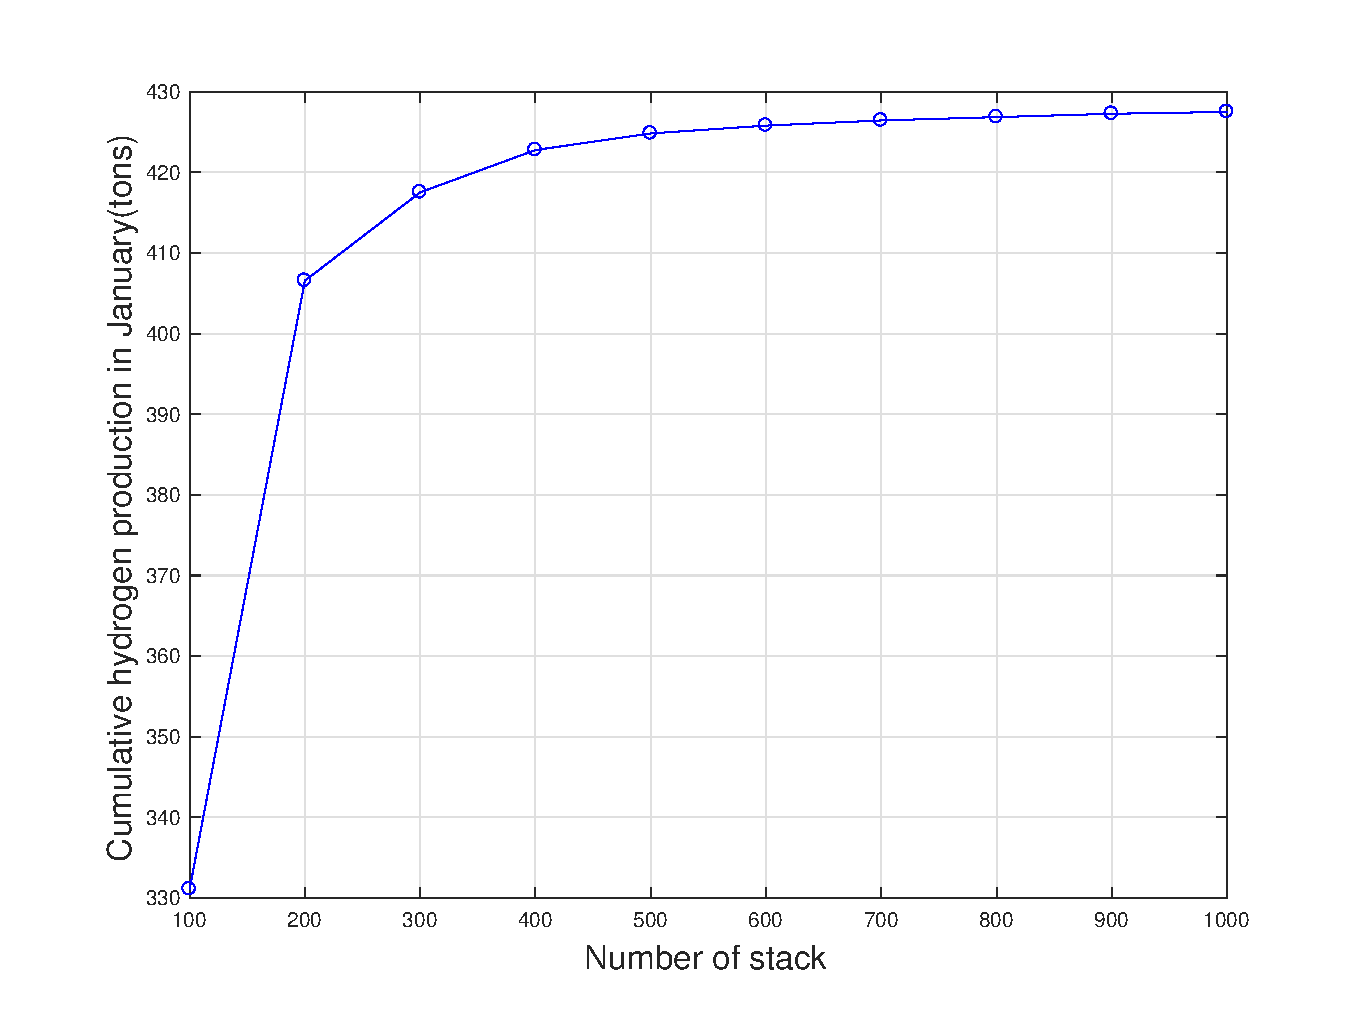
\includegraphics[width=7cm]{stack.eps}
\caption{Theoretical cumulative hydrogen production in January against number of stacks}
\label{fig:stack}
\end{figure}
 

\subsection{Thermal Model}
A lumped thermal capacitance model is established to determine the temperature of the electrolyte, which affects the V-I characteristics and system efficiency. The general energy balance can be represented by:\cite{reversible}
\begin{equation}
C_t\frac{dT}{dt} = \dot{Q}_{gen}- \dot{Q}_{exch}-\dot{Q}_{cool}
\end{equation}
where 
\begin{equation}
\dot{Q}_{gen} = N_c(U-U_{tn})I 
\end{equation}
\begin{equation}
\dot{Q}_{exch} = \dot{n}_{H_2} C_p^{H_2}(T - Ta) + \dot{n}_{O_2}C_p^{O_2}(T - Ta)+ \dot{n}_{H_2O}C_p^{H_2O}(T - T_{in}^w)
\end{equation}
\begin{equation}
\dot{Q}_{cool} = \dot{m}_fC_p^f(T_o^f - T_{in}^f) 
\end{equation}
where $\dot{n}_i$ is the molar flow rates of product gases and water, $\dot{m}_f$ is the mass flow rate of the cooling water. $N_c$ is the number of cells in series and $C_p^f$ is the thermal capacity of fluid at constant pressure. At steady state, $\frac{dT}{dt} = 0$,  thus the required cooling water flow rate can be calculated, which is around 9 tons per hour for each stack. The above equations can also be used to predict the time required for the electrolyte to be heated up to the required temperature, or used in temperature controller design which will be covered in the next session.

\subsection{Electrolyser Control System}
A control system needs to be installed in the electrolyser to keep it working properly. The CAD drawing at the start of this session included control logics such as temperature, pressure and level control.  A limiter is installed between the power source and electrolyser in order to prevent the low level power from passing through. The temperature control is designed to maintain the desired temperature. This can be achieved by controlling the flow rate of cooling water. Apart from the internal heat generated, a heater is also added as an additional heat source for better control. When the temperature is higher than the desired value, the cooling water flow rate increases to transfer heat more quickly.  Pressure is controlled to approximately 30 bar using pumps and pressure relief valves. Level controllers are installed in the electrolyser tank and gas-liquid separator to monitor the liquid level in the vessel to prevent leakage current and ensure that liquid in the separator is not carried to the next equipment. Due to space limit, only temperature control will be discussed here. Closed loop PID control is the control mode most often associated with temperature controllers.\cite{control} To achieve better performance, a fuzzy PID model is adopted here. It is based on PID control algorithm and fuzzy control algorithm, which achieves fuzzy adjusting the PID parameters.\cite{fuzzy} The Simulink model is shown in Figure \ref{fig:pid}. 
\begin{figure}[H]
\includegraphics[with=10cm]{fuzzypid.png}
\caption{Fuzzy PID block diagram}
\label{fig:pid}
\end{figure}
The four equations in the thermal model session can be used to determine the transfer function, which is in the form of 
\begin{equation}
G(s) = \frac{K}{T_s\times s +1} 
\end{equation}
In reality, there should also be a time lag $e^{-\tau s}$ term in the temperature control system. 
The comparison between traditional PID controllers and fuzzy PID controllers are shown in Figure \ref{fig:compare}.
\begin{figure}[H]
\centering
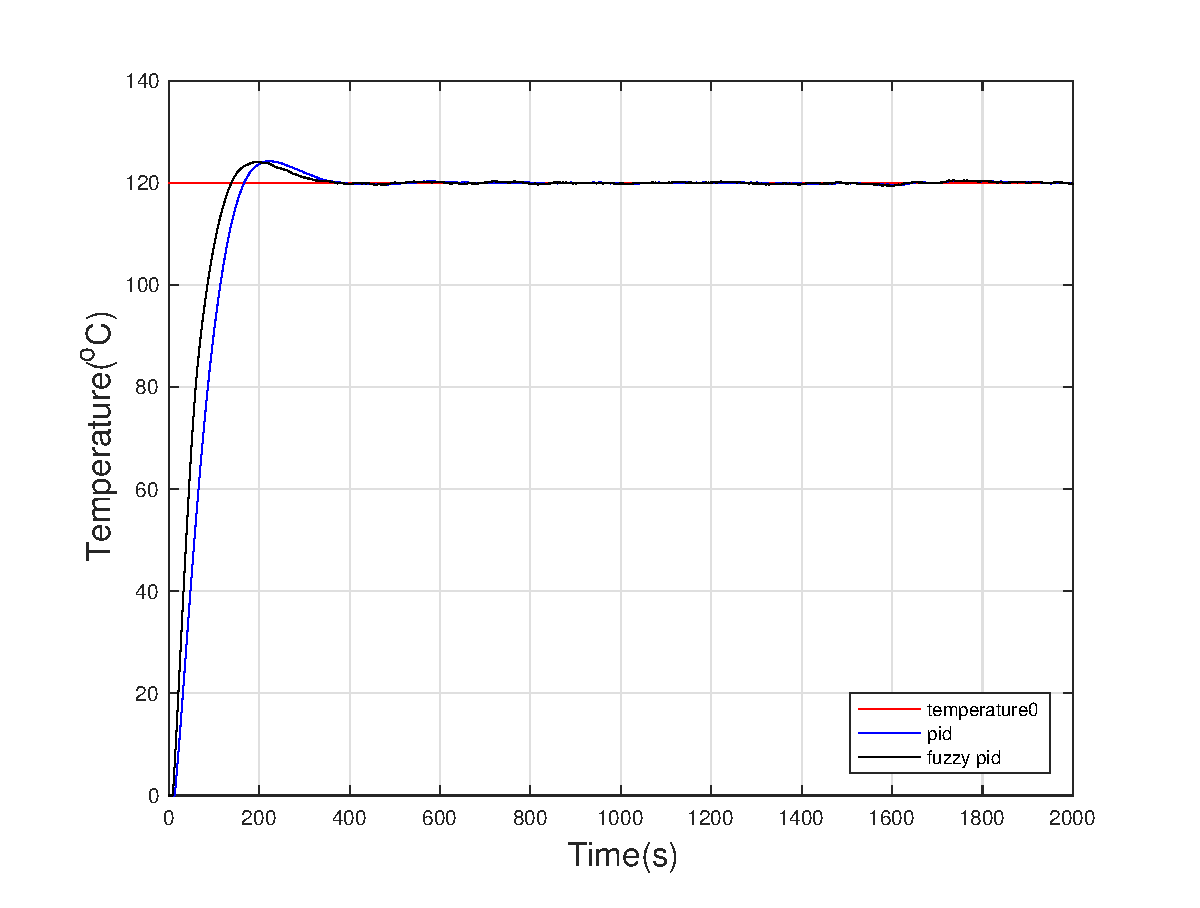
\includegraphics[width = 8cm]{pidpid.eps}
\caption{Comparison between PID and fuzzy PID controller under sensor noise}
\label{fig:compare}
\end{figure}
Both controllers have satisfactory performance with the fuzzy PID controller having faster response to changing temperature and smaller overshoot 



\subsection{Hydrogen  Storage }
The hydrogen storage system is required to supply the ammonia synthesis reactor with a constant hydrogen flow rate. There are three major ways to store the hydrogen gas produced , as compressed gas(above ground or underground), as a liquid or forming chemical bonding in solids(usually as metal hydrides).
When choosing a storage method, energy required, cost and safety are the major factors to consider and this is shown in Table \ref{tab:methods}.
\begin{singlespace}
\begin{table}[H]
\begin{tabular}{ |p{4.4cm}|p{2.4cm}|p{2.9cm}|p{3cm}| p{2.7cm}|} 
 \hline
  & Compressed Gas(700 bar) & Underground & Cryogenic Liquid   & Metal Hydride (NaAlH4) \\ 
 \hline
 Energy Required(MJ/kg) & 10.8  & 1.5  &43    & 15\\ 
 %\hline
 %Volumetric Energy Density(kWh/L) & 0.8 & 0 & 2.4 & 0.4\\
 \hline
Storage Cost(\$/kg) & 0.29  & 0.197  &1.48 & 0.116\\ 
 \hline
 Safety & High risk of fire or leak & Lower risk, potential leak due to cracks in rock & Risk of Overpressure & Zero Explosion Probability \\
 \hline
\end{tabular}
\caption{\label{tab:methods}Hydrogen storage method comparison\cite{gas2}\cite{gas3}\cite{storage}\cite{storage2}}
\end{table}
\end{singlespace}

Storage as a compressed gas using the gas steel cylinders is the most simple and commercially mature storage method, and is therefore adopted in this model. Isothermal compression($\Delta T = 0$) is the ideal case as it requires minimum work input compared with isentropic compression, which is adiabatic. Several stages of compression is adopted to achieve the required compression ratio (a final pressure of 700-800 bar with high strength materials) and the compressed gas needs to be cooled down after each stage.  The specific compression work can be calculated by \cite{gas}
\begin{equation}
w_i = RTZln(\frac{p2}{p1})
\end{equation}

where $Z$ is the compressibility factor, and it is used here since the compressed gas is non-ideal. $Z$  is a function of temperature and pressure but is assumed to be constant here for simplicity. $T$ is the temperature which is kept constant, $\frac{p2}{p1}$ is the compression ratio, where p1 is 30 bar. The compression work for different compression ratio is shown in Figure \ref{fig:compression}. At a final pressure of 700 bar, the compression work is 4.3 MJ/kg. In reality, the number should be higher than this since the process is not perfectly reversible or isothermal.(typical value is 10.8kJ/kg\cite{storage})

\begin{figure}[H]
\centering
\includegraphics[width=7cm]{compression.eps}
\caption{Compression work as a function of compression ratio}
\label{fig:compression}
\end{figure}

Underground storage in salt cavern has been developed for compressed hydrogen gas. It has the benefits of increased storage capacity, low cost and safer operation. However, if a cavern is not already available, the cost of digging and reinforcing can be quite high, and the storage location is also restricted by geological factors.\cite{cons} Although liquid hydrogen has a higher energy density compared with compressed gas, liquifying hydrogen is rarely adopted as a storage method since a large amount of energy is required to achieve a very low temperature(-252$^oC$), it also needs fairly expensive heat-insulating materials. Metal hydrides is formed when a host metal is bonded with hydrogen atom to form a compound. When hydrogen needs to be recovered, the compound is supplied with heat to break the bonds. This method can significantly increase the energy density and also has lower risk compared with other storage methods. However, the cost of storage is quite high and strongly bonded hydrogen is hard to be recovered.\cite{storage3}


\subsection{System Simulation}
A system simulation is carried out based on power input profile,  demonstrating the results for 120 hours in November 2016.  Figure \ref{fig:simulation}  shows the changes of  HHV efficiency and the ratio of power input and maximum input with time. As can be seen, the HHV efficiency is at a level of around 73\% for most of the time and increases when the power input is low. The gaps represent the time period when the power input is below the minimum allowed limit. Note that some power is lost during the AC to DC rectifier stage, the conversion efficiency is assumed to be 90\%. For simplification, the simulation assumed zero start-up time, zero response time and constant temperature at $120^oC$. Figure \ref{cumulative} demonstrates the cumulative production of hydrogen in this time period. Comparing this with the constant hydrogen consumption rate, the storage capacity requirement can be calculated. 
\begin{figure}[htb]
\centering
\includegraphics[width = 18cm]{simulation.eps}
\caption{HHV efficiency and Power/ Power max}
\label{fig:simulation}
\end{figure}

\begin{figure}[htb]
\centering
\includegraphics[width = 17cm]{cumulative.eps}
\caption{Cumulative production of hydrogen }
\label{cumulative}
\end{figure}

%\subsection{Auxiliaries}
%The water input to the plant needs to be pure, therefore a desalination process is required 


\subsection{Costing}
A rough capital cost estimate of the hydrogen production system is shown in Table \ref{tab:cost}. The total capital cost include direct field cost, indirect field cost and home office/miscellaneous cost. There will also be operating costs such as water and maintenance. Most materials need to be transported, installed and maintained, which would involve associated labour cost, it is assumed as 10\% of the material cost for static equipment, and 5\% for rotating equipment. The component costs are estimated from industry sources.\cite{cost} \cite{cost2} \cite{cost3}
\begin{singlespace}

\begin{longtable}{ |p{5.5cm}|p{2.5cm}|p{2.5cm}|p{2.9cm}|}
\caption{System Costings}
\label{tab:cost}
%\begin{table}[H]
%\begin{tabular}{ |p{5.5cm}|p{2.5cm}|p{2.5cm}|p{2.9cm}|} 
 \hline
 %champagne
 \rowcolor{champagne}
 %\rowcolor{burntsienna}
  & Labour \$ & Material \$ & Total \$\\
  \hline
  
  \rowcolor{blue-green}
   \multicolumn{4}{ | c |}{Direct Field Cost} \\
   \hline
  \rowcolor{LightCyan}
  \multicolumn{4}{ | c |}{Equipment Cost} \\
  \hline
  Vessels   & 19,380  & 193,800  & 213,180\\
  \hline
  Compressor & 421,550 & 8,431,000 & 8,852,550\\
  \hline
 Drums/Filters & 91,720  & 917,200 & 1,008,920\\
  \hline
  Stacks & 522,590 & 5,225,900 & 5,748,490 \\
  \hline
  Heat Exchangers & 5,100 & 102,000 & 107,100\\
  \hline
  Pumps & 735 & 14,700 & 15,435\\
  \hline
 
  %\rowcolor{cyan}
  \textbf{Subtotal Major Equipment} & \textbf{1,061,075} & \textbf{14,884,600} & \textbf{15,945,675}\\
   \hline
    \rowcolor{LightCyan}
   \multicolumn{4}{ | c |}{Bulk Material Cost} \\
   \hline 
    \multicolumn{4}{ | c |}{\textbf{Civil/Structure/Architectural}} \\
   %Civil/Structure/Architectural  \\
   \hline 
   Foundations & & 38,379  & 38,379\\
   \hline
   Roads/Pavings  & & 9,080  & 9,080\\
   \hline
Buildings &  &213,507  & 213,507\\
   \hline
   Structural Steels & & 16,350 & 16,350\\
   \hline
    \multicolumn{4}{ | c |}{\textbf{Piping/Instruments}} \\
   \hline
   Pipe & 4,605 & 46,050 & 50,655\\
   \hline
   Fittings & 1,235 & 12,350 & 13,585\\
   \hline
   Valves & 10,034 & 100,340  & 110,374\\
   \hline
   Cables & 3,805 & 38,050 & 41,855\\
   \hline
   Instruments & 2,270  & 22,701  & 24,971\\
   \hline
   Control Valves & 6,540 & 65,402 & 71,942\\
   \hline
    \multicolumn{4}{ | c |}{\textbf{Electrical}} \\
   \hline
   Cables &  3,405  & 34,050 & 37,455\\
   \hline 
   DCS cabinet & 6,502 & 65,020 & 71,522\\
   \hline
    \multicolumn{4}{ | c |}{\textbf{Paintings}} \\
   \hline
   Piping painting & 7,720 & & 7,720\\
   \hline
   Equipment painting & 12,350 & & 12,350\\
   \hline
   \multicolumn{4}{ | c |}{\textbf{Insulation}} \\
   \hline
   Piping Insulation & 27026 & & 27026\\
   \hline
   Equipment Insulation & 27026 & & 27026\\
   \hline
   \textbf{Subtotal Bulk Materials} & \textbf{58,466} & \textbf{661,279} & \textbf{719,745}\\
   \hline

   \textbf{Total Direct Field Materials} & \textbf{ 1,119,541} & \textbf{15,545,879} & \textbf{16,665,420}\\
   \hline
   \rowcolor{blue-green}
   %\rowcolor{cyan}
 \multicolumn{4}{ | c |}{Indirect Field Cost} \\  
 \hline
 Construction management & 45,403 & & 45,403\\
 \hline
 Cranes & 78,750 & & 78,750\\
 \hline
 Scaffolding & 40,646 & & 40,646\\
 \hline
\textbf{Total Indirect Field Costs} & \textbf{164,799
} & & \textbf{164,799
}\\
 \hline
 \hline
 \rowcolor{blue-green}
 %\rowcolor{cyan}
 \multicolumn{4}{ | c |}{Home Office/Miscellaneous} \\
 \hline
 Detailed Engineering & 41,818 & & 41,818 \\
 
 \hline
 
 
 Start-up & 12,121 & & 12,121\\
 \hline
\rowcolor{champagne}
 \textbf{Total Costs Excluding UAP} &  \textbf{1,338,279} & \textbf{15,545,879} & \textbf{16,884,158}\\
 \hline
 
Unallocated Provision  & & & 249,300\\
\hline
\rowcolor{champagne}
\textbf{Total Project Cost} & & & \textbf{15,795,179}\\
\hline
%\end{tabular}
\end{longtable}
\end{singlespace}

\subsection{Sustainability}
The Paris Agreement has set a target to limit the global temperature rise to 2$^oC$ above the pre-industrial level, corresponding to a
Carbon budget of 790GtC.\cite{sus} It has become a necessity for countries to develop long-term decarbonisation strategies. Therefore alkaline electrolysis derived by renewable energies has a great potential to become a more vital hydrogen production strategy due to its sustainable nature. Water is the only material input to the system and no greenhouse gases such as carbon dioxide will be produced in the process.The water The electricity comes from wind power station which is also sustainable. While alkaline electrolysis has a lower energy efficiency than the conventional hydrogen production methods such as natural gas reforming, the continuous advances in the electrolysis technologies could lower the production costs and make it more competitive and widely used in large scale projects.
\subsection{Safety}
The major risk in the electrolysis plant is the flammable mixture of oxygen and hydrogen gases.
Hydrogen has the NFPA 704's highest rating of 4 on the flammability scale. \cite{safety} This can happen if the gas crossover during the electrolysis is above the allowed limit, or if hydrogen is leaked to the air which is difficult to detect since its colourless, odourless, and tasteless. Hydrogen gas has a flammability range of 4-75\% in the air and it also has a very low ignition energy(as low as 17$\mu$J).To avoid this problem, 
before driving the hydrogen production equipment, it is necessary to fill the system with nitrogen until the oxygen content of the system is less than 1\%; Hydrogen leak alarm devices need to installed and electrolysis room should be set explosion-proof lights. Hydrogen flames are also nearly invisible, so flame detectors are needed. Also, all the equipment should be well grounded to prevent static electricity, which can cause hydrogen combustion and explosion. The leakage of the alkaline electrolyte is another potential risk. The HAZOP analysis is shown below.


{\fontsize{8pt}{7.5pt}\selectfont\tabcolsep=2.5pt\renewcommand\arraystretch{1.5}
\begin{longtable}{
|m{1.75cm}<{\centering}|m{3.1cm}<{\centering}|m{4.5cm}<{\centering}
|m{1.25cm}<{\centering}|m{1.1cm}<{\centering}
|m{4cm}<{\raggedright}|}
\caption{HAZOP Analysis}
 \hline
 \rowcolor{LightCyan}
Deviation &Causes &Unmitigated Consequences &Likelihood &Risk Ranking &Recommendations\\
\hline
\multirow{11}*{More Flow} & {Hydrogen/oxygen control valve failure} &
{Cell reaction pressure drop, Electrolysis efficiency will be affected} & Middle & Low & Add high flow alarm to respond\\
\cline{2-6}
&{Cooling Water hand valves fully open by human error} &
No Hazard identified &&&\\
\cline{2-6}
&{Caustic control valve failure} &
{High level in cell, lead to overpressure, potential fatality} &
 Low & \multicolumn{1}{>{\columncolor{red}}c|}{High} &
{Add high level alarm to respond; \par
Add high high level interlock to
trip reaction cell.}\\
\cline{2-6}
&{Feed water valve fully open by human error} &
{Flooding in the separator} &
 Low & Low & Add high level alarm to respond;\\
\cline{2-6}
&{Nitrogen hand valve open by human error} &
Production unqualified. & Low &Low &
{Add blind flange between the two hand valves.}\\
\hline
\multirow{13}*{Less Flow}&
{Hydrogen/oxygen control valve failure} &
{Overpressure;lead to vessel/cell rupture; potential fatality} &
 Low & \multicolumn{1}{>{\columncolor{red}}c|}{High} & {Add high pressure alarm to respond; \par
Add high Pressure interlock
to trip reaction cell.}\\
\cline{2-6}
&{Cooling Water hand valves fully closed by human error} & {Material corrosion; mechanical failure; production unqualified} &  Low & Middle & {Add high temperature alarm for the production to response}\\
\cline{2-6}
&{Caustic control valve failed; fully closed} & {Low level in cell, lead to reaction stop; leakage current} &  Low & Middle &Add Low level alarm to respond.\\
\cline{2-6}
&{Feed water valve fully closed by human error} & {Low level in cell, lead to reaction stop} &  Low & Low & Add Low level alarm to response.\\
\hhline{~|-----}
&Pump Failure &
{Backflow of gases, causing flammable gas mixture} &  Low & \multicolumn{1}{>{\columncolor{red}}c|}{High} & Use valves to prevent gas backflow\\
\hhline{~|-----}
&Facility Leakage & {Hydrogen leak into facilities, risk of explosion} &  Low & \multicolumn{1}{>{\columncolor{red}}c|}{High} & { Install hydrogen sensor and leak alarm for emergency shut down}\\
\hhline{~|-----}
&Valve or pipe blockage & Bursting of pipes &Low &\multicolumn{1}{>{\columncolor{red}}c|}{High} &Install blockage detectors\\
\hhline{~|-----}
&Water level too low & Leakage current & Low &\multicolumn{1}{>{\columncolor{red}}c|}{High} &Check the level controller\\
\hline
No flow &\multicolumn{5}{c|}{Refer to less flow}\\
\hline
\multirow{4}*{Reverse Flow}& {Caustic source shut down due to unknown reason} & {Hydrogen reverse to caustic system, causing jet fire if leaked, potential people injury} & Low & Middle & Add check valve.\\
\cline{2-6}
&{Feed water source shut down due to unknown reason} & {Hydrogen reverse to feed water system, causing jet fire if leaked, potential people injury} & Low & Low & Add check valve.\\
\hline
High Pressure & {Pressure control system fails; Blockage; Pump failures} & {Facilities breakdown, potential explosion; low gas purity} &  Low & \multicolumn{1}{>{\columncolor{red}}c|}{High} &
Pressure sensor installed for
emergency shutdown\\
\hline
Low Pressure& Pump fails; pressure controls fails; leak in reactor& Electrolyte boils if operating above 100$^\circ$C; more work at hydrogen storage stage &  Low & Middle &
Check the pumps; \par
Check for any leakage\\
\hline
High Temperature & Cooling water flow rate too low; Heat exchanger malfunction&
Material corrosion and mechanical failure such as membrane rupture;
Electrolyte boiling& Low &\multicolumn{1}{>{\columncolor{red}}c|}{High}&
Check the cooling water
valves \par
Check temperature controller\\
\hline
Low Temperature & Cooling water flow rate too high; Heat exchanger malfunction& Low efficiency &Low &Low &
Check the cooling water valves \par
Check temperature controller\\
\hline
Rupture/ Leak &Tube rupture in cooler& High pressure cooling water, could cause jet fire if leaked& Low &Middle &Add pressure relieve valves\\
\hline
Contaminants/ Composition& Water deionization stage
malfunction&
Side reactions; reduce lifetime &Low &Middle& Add anaylser for feed water quality\\
\hline
Chemical Hazards& Electrolyte concentration too high& Cell or pipeline leakage;corrosion of membrane and electrodes& Low &\multicolumn{1}{>{\columncolor{red}}c|}{High}&
Upgrade materials. \par
Check recirculation pump \par
Install PH meter linked to alarms\\
\hline
\end{longtable} }
%\includepdf[pages=2,angle=180]{hazop.pdf}
%\includepdf[pages=3,angle=180]{hazop.pdf}




\subsection{Conclusion} 
Alkaline electrolysis integrated with wind energy to produce hydrogen is a mature technology with a great potential to reach a larger production scale.
The system performance can be improved by operating at elevated pressures and temperatures, as well as adopting the latest technology such as zero-gap configuration. The materials chosen are both cost-effective and able to maximize efficiency. The system is able to produce hydrogen gas at a high purity with an HHV efficiency of around 73\%, and is able to respond to dynamic wind power input with a wide load range. The plant is sustainable and generally cost-effective. With the continuous development of more advanced electrolysis technology and the upward trend of using renewable energies globally, the system will be able to operate at a higher efficiency and larger scale to become more competitive than the traditional hydrogen production methods.



\singlespacing
%\linespread{0.4}
\begin{thebibliography}{99}
\linespread{1} 
\bibitem{reversible}
M. Hammoudi, C. Henao, K. Agbossou, Y. Dube, M.L. Doumbia, New multi-physics approach for modelling and design of alkaline electrolyzers
\bibitem{gibbs} 
Joonas Koponen, Review of water electrolysis technologies and design of renewable hydrogen production systems
\bibitem{gas}
Hydrogen Science and Engineering, Materials, Processes, Systems and Technology, Wiley-VCH
\bibitem{specification}
Study on development of water electrolysis in the EU Fuel Cells and Hydrogen Joint Undertaking
\bibitem{purity}
V. L. KuchaevE. N. ShapatinaA. K. Avetisov, Mechanism of oxygen poisoning of ammonia synthesis catalyst
\bibitem{conductivity}
R.J. Gilliama,, J.W. Graydonb, D.W. Kirkb, S.J. Thorpea, A review of specific conductivities of potassium hydroxide solutions for various concentrations and temperatures
\bibitem{activation4}
Christian Henao, Kodjo Agbossou, Mhamed Hammoudi, Yves Dub, Alben Cardenas, Simulation tool based on a physics model and an electrical analogy for an alkaline electrolyser
\bibitem{activation}
Richard L. Doyle and Michael E.G. Lyons, The Oxygen Evolution Reaction: Mechanistic Concepts and Catalyst Design
\bibitem{activation1}
Milewski, J, Guandalini, G  Campanari, S 2014, Modeling an alkaline electrolysis cell through reduced-order and loss-estimate approaches?, Journal of Power Sources, vol. 269, pp. 203211.
\bibitem{activation2}
Hammoudi, M, Henao, C, Agbossou, K, Dub, Y, Doumbia, M 2012, New multi-physics approach for modelling and design of alkaline electrolyzers, International Journal of Hydrogen Energy, vol. 37, no. 19, pp. 1389513913.
\bibitem{bubble2}
H.Vogt, R,J, Balzer, The bubble coverage of gas-evolving electrodes in stagnant electrolytes
\bibitem{void}
Kitipong Tangphanta, Kaokanya Sudapraserta, z, and Suthin Channarong,Mathematical Modeling of Electrical Conductivity
in Electrolyte Solution between Two Gas Evolving Electrodes
\bibitem{currentdensity}
Kai Zeng 1, Dongke Zhang,Recent progress in alkaline water electrolysis for hydrogen production and applications
%\bibitem{currentdensity2}
%Ugljesa Babic, Michel Suermann, Felix N. B�chi, Lorenz Gubler, Thomas J. Schmidt, Critical Review?Identifying Critical Gaps for Polymer Electrolyte Water Electrolysis Development
\bibitem{temp}
R. L. LERoY, INDUSTRIAL WATER ELECTROLYSIS: PRESENT AND FUTURE
\bibitem{efficiency2}
Alfredo Ursua, Member IEEE, Luis M. Gand, and Pablo Sanchis, Member IEEE, Hydrogen Production From
Water Electrolysis: Current Status and Future Trends
\bibitem{efficiency}
RodneyL. LeRoy andChristopherT. Bowen, The Thermodynamicsof AqueousWater Electrolysis
\bibitem{configuration2}
Tilak, B, Lu, P, Colman, J,  Srinivasan,  1981, Chapter 1  Electrolytic production of hydrogen, in: Bockris, J, Conway, B, Yeager, E \& White, R, Comprehensive treatise of electrochemistry, volume 2: Electrochemical processing, Plenum Press, New York.
\bibitem{configuration}
A. Ursua, B, Hydrogen production with alkaline electrolyzers: Electrochemical modelling, electric power supplies
and integration with renewable energies,[ (in Spanish) Ph.D. dissertation, Dept. Electr.
\bibitem{zerogap}
Robert Phillips,a and Charles W. Dunnill,  Zero Gap Alkaline Electrolysis Cell Designs for
 Renewable Energy Storage as Hydrogen Gas
\bibitem{geometry}
N. Nagai, M. Takeuchi,T. Kimura, T. Oka, Existence of optimum space between electrodes on hydrogen production by water electrolysis
\bibitem{anode}
D. E. Hall, Electrodes for Alkaline Water Electrolysis, Inco Research \& Development Center, Incorporated, Sterling Forest, Suern, New York 10901
\bibitem{anode2}
D. E. Hall, Alkaline Water Electrolysis Anode Materials, American Cyanamid Company, Chemical Research Laboratories, Stamford, Connecticut 06904
\bibitem{cathode2}
Kjartansdttir, Cecila Kristn; Moller, Per, Development of Hydrogen Electrodes for Alkaline Water Electrolysis
\bibitem{cathode}
High-efficiency and stable alloyed nickel based electrodes for hydrogen evolution by seawater splitting, Zhang,Li,Yang,Fa,Ge. Journal of Alloys and Compounds.732 (2018) 248-256
\bibitem{ionic}
Ivana M.PerovicPetar Z.LausevicGvozden S.TasicBojan B.RadakVladimir M.Nikolic,Sladjana Lj.MaslovaraMilica P.Marceta Kaninsk, Novel ternary Ni-Co-Mo based ionic activator for efficient alkaline water electrolysis
\bibitem{zirfon}
Ph. VERMEIREN, W. ADRIANSENS, J. P. MOREELS and R. LEYSEN,  EVALUATION OF THE ZIRFONj SEPARATOR FOR USE IN ALKALINE WATER ELECTROLYSIS AND Ni-H, BATTERIES
\bibitem{pressure}
Nicolas Guillet and Pierre Millet, Alkaline Water Electrolysis
\bibitem{ionexchange}
Hanna Jaroszek, Piotr Dydo, Ion-exchange membranes in chemical synthesis, a review


\bibitem{separator}
Diogo M. F. SantosI,; Csar A. C. SequeiraI; Jose L. Figueiredo, Hydrogen production by alkaline water electrolysis
\bibitem{separator3}
YEO, S. C.  EISENBERG, A. 1977. Physical Properties and Supermolecular Structure of Perfluorinated
Ion-Containing (Nafion) Polymers. Journal of Applied Polymer Science, 21, 875-898.
\bibitem{separator2}
Karel Vazac, Martin Paidar, Martin Roubalk, Karel Bouzek, Impact of the Cation Exchange Membrane Thickness on the Alkaline Water Electrolysis
\bibitem{ultrasound}
Sheng-De Li, Cheng-Chien Wang, Chuh-Yung Chen,Zhancheng Guo, Water electrolysis in the presence of an ultrasonic field
\bibitem{review}
Mingyong Wang,Zhi Wang,Xuzhong Gong ,The intensification technologies to water electrolysis for hydrogen production

\bibitem{control}
Appendix F:PID Temperature Control https://www.lakeshore.com/Documents/LSTC\_appendixF\_l.pdf
\bibitem{fuzzy}
WANG Haiqing, JI Changying, LIU Tongzhao, GAO Feng, XIAN Jieyu, Modeling and Simulation ofFuzzy Self-tuning PID Temperature Control System


\bibitem{gas2}
Zehra Yumurtac and Nur Bekiroglu, Yildiz Technical University Mechanical Engineering Faculty, TR 34349, Besiktas Istanbul, ECONOMICAL
ANALYSIS OF GASEOUS AND LIQUID HYDROGEN STORAGE AND TRANSPORTATION
\bibitem{gas3}
L. Kit Heung, L. Kit Heung, Savannah River Technology Center Aiken, SC 29808 USAUsing Metal Hydride to Store Hydrogen
\bibitem{storage}
Monterey Gardiner, Energy requirements for hydrogen gas compression and liquefaction as related to vehicle storage needs, https://www.hydrogen.energy.gov/pdfs/9013\_energy\_requirements\_for\_hydrogen\_gas\_compression.pdf
\bibitem{storage2}
L. Kit Heung Savannah River Technology Center Aiken, SC 29808 USA, Using Metal Hydride to Store Hydrogen, https://pdfs.semanticscholar.org/b781/192e2624db103d1b615502dd44354eff9b52.pdf




\bibitem{cons}
Above Ground Vs. Underground Storage Tanks: Pros and Cons,http://www.communicationsetc.net/above-ground-vs-underground-storage-tanks-pros-and-cons/
%\bibitem{rate} 
%Alhassan Salami Tijania, Nur Afiqah Binti Yusupb, A. H. Abdol Rahimc
%\textit{The \LaTeX\ Companion}. 
%Mathematical modelling and simulation analysis of advanced alkaline electrolyzer system for hydrogen production

%\bibitem{thermoneutral}
%Allebrod, Frank; Mogensen, Mogens Bjerg; Hjelm, Johan; Ebbesen, Sune Dalgaard, High Temperature and Pressure Alkaline Electrolysis




%\bibitem{activation3}
%H. Wendt and V. Plzak. Electrocatalytic and thermal activation of anodic oxygen- and cathodic hydrogen-evolution in alkaline water electrolysis. Electrochimica Acta, 28(1):27?34, 1983.


%\bibitem{geometry}
%N. Nagai, M. Takeuchi,T. Kimura, T. Oka, Existence of optimum space between electrodes on hydrogen production by water electrolysis
%\bibitem{zerogap}
%A.Ursua.Hydrogen Production From Water Electrolysis: Current Status and Future Trends Proceedings of the IEEE 100(2):410-426February 2012
%\bibitem{bubble}
%H.Vogt, The actual current density of gas-evolving electrodes Notes on the bubble coverage

%\bibitem{void2}
%Bhanu kiran.A1, Y.V.Ramana murty, Mathematical Modelling and Simulation Analysis of Alkaline Water Electrolyser for Stationary Electrolyte in Atmospheric Pressure

%\bibitem{pressure}
%Nicolas Guillet and Pierre Millet, Alkaline Water Electrolysis
%\bibitem{pressure2}
%Joonas Koponen, Review of water electrolysis technologies and design of renewable hydrogen production systems


%\bibitem{membraneless}
%M.I. Gillespiea, R.J. Kriek, Hydrogen production from a rectangular horizontal filter press Divergent Electrode-Flow-Through (DEFTTM) alkaline electrolysis stack
%\bibitem{membraneless2}
%M.I. Gillespie, F. van der Merwe, R.J. Kriek, Performance evaluation of a mem-
%braneless divergent electrode-flow-through (DEFT) alkaline electrolyser based on optimisation of electrolytic flow and electrode gap, J. Power Sources 293 (2015) 228?235.

















\bibitem{storage3}
Wade A. Amos, National Renewable Energy Laboratory, Costs of Storing and Transporting Hydrogen
\bibitem{cost}
David Milligan and Judy Milligan. Matches’ process equipment cost estimates. [Online] http: //matche.com/equipcost/Default.html, 2014. [Accessed 10/4/18].
\bibitem{cost2}
http://kkft.bme.hu/htms/kornykozp/Cost.of.Equipments.pdf. [Accessed 15/4/18]
\bibitem{cost3}
L. Bertucciolo, E. Chan, D. Hart, F. Lehner, B. Madden, and E. Standen, “Development of Water Electrolysis in the European Union: Final Report,” Fuel Cells and Hydrogen Joint Undertaking, Final Report, Feb. 2014.
\bibitem{sus}
Kentaro Tamura, PhD Leader, Climate and Energy Area
Institute for Global Environmental Strategies (IGES),Paris Agreement: From Low Carbon to Decarbonization.
\bibitem{safety}
https://en.wikipedia.org/wiki/Hydrogen\_safety [Accessed 15/4/18]



\end{thebibliography}

\end{document}








% Haber Chapter
%\lfoot{James Rhodes}
%\graphicspath{{./ammoniasynth/graphics/}}
%%\documentclass[11pt, a4paper]{article}

%\title{Ammonia Synthesis}
%\author{James Rhodes}
%\date{\today}

%\usepackage{fullpage}
%\usepackage{mhchem}
%\usepackage{setspace}
%\usepackage{inputenc}
%\usepackage{wrapfig}
%\usepackage{textcomp}
%\usepackage{graphicx}
%\usepackage{pdflscape}
%\usepackage{wrapfig}
%\usepackage{mathtools}


%\usepackage{graphicx}
%\graphicspath{ {graphics/} } 
%\linespread{1.5}



\newcommand\tc{400}
\newcommand\pbar{150}
\newcommand\ammOUT{227.6}  %daily average ammonia production requirement tonnes/day
\newcommand\conv{28}	%first pass conversion rate
\newcommand\purge{5}



%\begin{document}

%\maketitle
%\tableofcontents

%\doublespacing
\section{Ammonia Synthesis}
\subsection{Introduction}


\subsubsection{Overview}
The production process of ammonia is a key stage in converting the hydrogen gas produced in electrolysis and nitrogen from cryogenic separation of air into liquid ammonia. This is useful as it is significantly safer and cheaper to store long-term than hydrogen this is due to the significantly lower boiling point of hydrogen and thus the lower energy density of hydrogen at atmospheric conditions (2.96 MJ/L) compared to that of ammonia (13.77 MJ/L)\cite{Bartels2008} thus a not only would a volume 4.65 times greater than that of ammonia would be required for comparable energy storage. Significantly higher pressures and cryogenic temperatures would be required to store hydrogen in liquid form, making large quantities significantly more expensive to store.
\\
Stored ammonia can then be fed to the power generation side of the plant in order to match  the power demand of the region, and provide long term storage for renewable wind energy without the need for the combustion of fossil fuels.

In order to produce ammonia a reversible reaction takes place between hydrogen and nitrogen. The equation of reaction for ammonia synthesis from nitrogen and hydrogen is;

\begin{equation}
3H_2+N_2   \underset{ }{\stackrel{ }{\rightleftharpoons}}   2NH_3 \qquad \Delta h_0 = -92.44 \; kJ/mol 
\end{equation}

This synthesis reaction is exothermic and can be designed in such a way that the high temperature products of reaction can be used to preheat the reactants to the operating point of reaction in an auto-thermal process. This has significant benefits in terms of reducing the energy requirements of the plant. However, the process by which the reaction takes place can vary depending on the requirements of the plant.

\subsubsection{Design objective}
The ammonia synthesis stage of the plant design was required to meet the capacity of ammonia production for the storage of excess energy produced by the wind turbines. This can subsequently be stored as liquid ammonia and be used to generate electricity in the solid oxide fuel cell and gas turbine in order to match the fluctuating electricity demand of the region. A number of different methods of ammonia synthesis have been reviewed and considered in the design process in order to design a process best suited to the scale, technology, economic constraints and environmental impact of plant. 
\\
In regard to the scale, of the process an initial year long demand requirement for stored energy was calculated in the control and energy matching design process [REFERENCE WILL] this g both a requirement for the year-long average energy demand for stored ammonia as well as the maximum energy storage requirement cause by a supply/demand deficit. 
These requirements are shown in table \ref{req} below, using the known efficiencies of the power generation stages and their respective duties an annual demand for ammonia can be calculated. Supply-demand matching can also be used to calculate the maximum storage required throughout the year. This gives scale requirements for ammonia output and storage and thus the design requirements for my design process. 

As defined by the power demand of Maui, Hawaii the year average power is set to average at a plant output of $36.6MW$. Accounting for combined generation efficiency in the ammonia-to-power stage of $61.7\%$ this translates into a daily average ammonia output of $\ammOUT$ metric tonnes. However, this does not account for the variable supply of wind power and subsequent hydrogen. Thus the ammonia synthesis stage must be designed for a higher capacity to ensure that it can adjust to temporal fluctuations in energy supply. Thus a reactor with a capacity for $300$ tonnes per day will be designed with short term hydrogen storage and an an ammonia breakdown loop to ensure continuous operation of the synthesis process. 
\begin{table}[!htbp]
	\begin{center}
		\label{req}
		\caption{Design requirements of synthesis stage}
		
		\begin{tabular}{|c|c|c|c|}
			\hline
			Yearly output& Average output & Storage required & Power stage efficiency     \\ \hline
			83058 tonnes            & $\ammOUT $  tpd            & 15000 tonnes                          & 61.7 \%  \\ \hline
		\end{tabular}
		
	\end{center}
\end{table}


Further considerations were given to technological requirement, whilst new and emerging technologies were considered in the design process priority was given to methods that have been successfully implemented on medium and large scale processes, laboratory condition processes whilst considered were only chosen if there was a clear method in upscaling to industrial levels and the benefits of doing so were significantly greater than established industrial processes. This was due to the need for reliability of power supply, especially considering the island location of the power plant and the lack of alternative power sources.
Finally, consideration was given to the environmental and economic considerations. These were especially important if the plant was going to have to provide clear benefits over gas and coal power generation plants. Thus the impact of waste flows was considered heavily as was the opportunities to recycle materials where possible. 



\subsection{Review of ammonia synthesis methods}


\subsubsection{Haber process}
The most well established and widely used method for producing Ammonia is the process developed on an industrial scale in 1913 by Fritz Haber at BASF. This involved the reaction of N$_2$ and H$_2$ feed gases over a hetrogenous solid iron catalyst at high temperature and high pressure. The most common catalyst in this process is Fe in magnetite form. Whilst this process is well established and easily scalable with current production capacities exceeding 3000tpd \cite{Banares-alcantara2014} its low single pass conversion and large ramp-up time makes it difficult for demand matching, meaning the process is usually run as a continuous process. Despite this limitation a large number of research and improvements have been made to this process and with the addition of a recycle stream overall conversion rates above 95\% are now regularly achieved. Developments into the catalyst composition used in the reactor has led to lower pressure reactors and higher single pass conversion rates.

Perhaps the most significant of these has been the development of w\"{u}stite as an alternative to magnetite as the iron precursor in the catalyst. This has shown clear advantages in terms of ammonia first pass conversion at lower temperatures and pressures and for similar material promoters\cite{Pernicone2003} \cite{Liu1996}.


\subsubsection{Ruthenium-based synthesis}

A growing competitor to the iron-based synthesis route is an ammonia synthesis production route in which a Ruthenium based catalyst is used in place of the iron. Despite know usage in ammonia synthesis since 1917 it was not until 1972 that Ozaki et al demonstrated visibly higher activity in ammonia synthesis converters using Ru as an active component. This had led to field of research into its use as a catalyst and in 1992 the development of the KAAP (Kellogg Advanced Ammonia Process) industrial process for Ru-based ammonia synthesis \cite{Rossetti2006}. This process is typically able to operate under significantly lower pressures and feed ratios than iron-based catalysts, meaning a clear economic advantage in terms of reactor and pressure vessel design. The tradeoff is the scarcity of Ruthenium and thus the significantly higher cost of the catalyst. This can be shown in Table \ref{tab:cat} below \cite{Liu2014}.
{\renewcommand{\arraystretch}{1.4}
\begin{table}[!htbp]
	\begin{center}
	\label{tab:cat}
\caption{Comparison of ammonia synthesis catalysts}

	\begin{tabular}{|c|c|c|c|c|c|}
	\hline
	Catalyst& Availability & Cost (USD/m$^3$)* & T/ \textdegree C     & H$_2$/N$_2$ ratio & Energy consumption (Gj/t) \\ \hline
	Fe            & abundant              & 4750                          & 350-525 & 2-3             & $\sim$27                      \\ \hline
	Ru            & scarce                & 254100                        & 325-450 & under 2         & $\sim$27                      \\ \hline
\end{tabular}
{\small *converted from CNY data at March 2018 exchange rates}

\end{center}
\end{table}

The cost of Ruthenium being over 50 times greater than that of Iron is a huge factor in the cost of the reactor. Furthermore, the poisoning of the Ruthenium by high concentrations of hydrogen can mean the cost of replacing the catalyst.

\subsubsection{Electrocatalysis}
An alternate method of producing ammonia is to use electrocatalysis reaction. This is a non-spontaneous thermodynamic reaction:
\begin{equation}
3H_2O+N_2   \underset{ }{\stackrel{ }{\rightleftharpoons}}   2NH_3 + 1.5O_2 \qquad (K_{298} = 10^{-120})
\end{equation}	
This can occur using electric energy. This has shown similar efficiency to established synthesis methods under normal temperatures and pressures \cite{Liu2014}. In recent years this has been a growing field with research into materials for electro-catalysts and electrolytes. However, current limitations of low current efficiency and conversion rates make this technology one in need of further development. Despite this the process has some clear benefits, the main one being the use of water as a hydrogen source reduces the need for hydrogen production; enabling the direct conversion of  wind-generated electrical energy into ammonia.
{\begin{figure}[h]
		\centering
		\caption{Electrochemical ammonia synthesis - anode (l), cathode(r)  \cite{Kyriakou2017}}
		{\centering
			
			\includegraphics[scale=0.65]{electrochemical_synthesis}
			\includegraphics[scale=0.7]{electrochemical_synthesis2}	
	}
%source https://ac.els-cdn.com/S0920586116304138/1-s2.0-S0920586116304138-main.pdf?_tid=04f1f2e8-973d-448d-aadd-175ff2e8e895&acdnat=1523822193_0cdd35a3744e5241062382a77c9c5f63%
\end{figure}}



\subsubsection{Photocatalytic synthesis}
Using the same principles of photosynthesis the photocatalytic reaction of nitrogen and water to form ammonia and oxygen can be achieved at room temperature and atmospheric pressure under the addition of solar energy. However, despite ongoing research into this field and a number of photocatalysts available, the scale of this process would currently be unable to meet the ammonia requirement of the plant\cite{Liu2014}.


\subsection{Thermodynamic modelling}

\subsubsection{Equilibrium constant}

The equilibrium constant for ammonia synthesis was first calculated by Gillespie and Beattie (1930)\cite{Gillespie1930} and is a function of the reaction temperature.
\begin{equation}
logK_a = -2.691122log(T) - 5.519265\times10^{-5}T + 1.848863\times10^{-7}T^2+\frac{2001.6}{T}+2.6899
\end{equation}
{\begin{figure}[h]
\begin{center}

		\caption{Equilibrium constant K$_a$ of ammonia synthesis reaction at varying temperature}


\includegraphics[scale=0.6]{K_a_varying_temperature}
\end{center}
\end{figure}}

This suggests that a lower temperature produces a higher equilibrium constant, as ammonia synthesis is an exothermic reaction theory supports this result as an exothermic reversible reaction favours the reactants as temperature increases.

\subsubsection{Reaction mixtures}
When calculating the properties of reaction mixtures throughout the system a rule of mixtures is used. Eqn. \ref{cpmix} gives the specific heat of a reaction mixture where $x_{i}$ are the mole fractions in the stream and $C_{p,i}$ are their respective specific heats. 
\begin{equation}
\label{cpmix}
	C_{p,mix} = x_{N_2}C_{p,N_2} + C_{p,H_2} + C_{p,NH_3}
\end{equation}
Calculating the respective specific heats  $C_{p,i}$ can be given by the polynomial temperature correlation Eqn. \ref{cp}.
\begin{equation}
\label{cp}
C_{p,i} = a + bT + cT^2 + dT^3
\end{equation}
\begin{table}
\caption{Specific heat coefficients \cite{Morgan2013}}
\label{cpco}
	\begin{center}
		 \begin{tabular}{|l|l|l|l|}
		\hline
			Coefficient & 
			N$_2$               & H$_2$               & NH$_3$              \\
			\hline
			a           & $28.9$               & $29.11$              & $27.568$             \\
			\hline
			b           & $-0.1571*10^{-2}$ & $-0.1916*10^{-2}$ & $2.5630*10^{-2}$  \\ \hline
			c           & $0.8081*10^{-5}$  & $10.4003*10^{-5}$  & $0.99072*10^{-5}$ \\
			\hline
			d           & $-2.873*10^{-9}$  & $-0.8704*10^{-9}$ & $-6.6909*10^{-9}$ \\
			\hline
		\end{tabular}
	
	\end{center}
\end{table}

\subsection{Mechanism and Kinetics}

\subsubsection{Reaction mechanism}

The reaction mechanism of the ammonia synthesis stage was key in understanding the kinetics of reaction and the effectiveness of a catalyst. This is due to the need for the $N_2$ bond to be broken on the surface of the catalyst during adsorption but also for the need for the dissociation of the bond during the synthesis step. The established mechanism steps for the ammonia synthesis reaction is understood to be the following reaction \cite{Jennings1991}.
\begin{subequations}
	\label{mech}
\begin{align}
H_2+*   &\underset{ }{\stackrel{ }{\rightleftharpoons}}   2H_{ad}\\
N_2+*   &\underset{ }{\stackrel{ }{\rightleftharpoons}}   N_{2,ad}\\
N_{2,ad}   &\underset{ }{\stackrel{ }{\rightleftharpoons}}   2N_{ad}\\
N_{ad}+H_{ad}   &\underset{ }{\stackrel{ }{\rightleftharpoons}}   NH_{ad}\\
NH_{ad}+H_{ad}   &\underset{ }{\stackrel{ }{\rightleftharpoons}}   NH_{2,ad}\\
N_{2,ad}+H_{ad}   &\underset{ }{\stackrel{ }{\rightleftharpoons}}   NH_{3,ad}\\
N_{3,ad}   &\underset{ }{\stackrel{ }{\rightleftharpoons}}   NH_{3}+*
\end{align}
\end{subequations}
Where $*$ denotes the forming of an adsorption site. Experimental studies have found the adsorption of nitrogen (\ref{mech}b) to be the rate determining step in this process and thus leading to an understanding of the microkinetics of the rate of reaction. This is due to the strong N$_2$ triple bond that must be broken.

%As the reaction is exothermic an increase in temperature would favour the reactants over the products. Experimental studies have confirmed this. The equilibrium constant $K_a$ can be found using the Gillespie and Beattie equation;
%


\subsubsection{Rate of reaction}

Numerous models \cite{Aparicio2008} for the rate of reaction of ammonia synthesis, however, the most widely used model for the rate of reaction is the Temkin equation \cite{Guacci1977}. Whilst a number of different forms of the equation have now been developed the Dyson and Simon \cite{Dyson1968} form is preferred in this analysis due to its simplicity and the limited experimental data required to simulate results.

\begin{equation} r_{NH_3} = K_2 \left [ K_a^2 \times f_{N_2}
\left ( \frac{f_{H_2}^3}{f_{NH_3}^2} \right ) ^\alpha - \left ( \frac{f_{NH_3}^2}{f_{H_2}^3} \right ) ^{\alpha - 1}
\right ]
\end{equation}

This equation the fugacities, $f$, rather than partial pressures have been used. Whilst the values of the equilibrium constant $K_a$ is well known the constant of reverse reaction $K_2$ and empirical constant $\alpha$ are found experimentally.

{\begin{figure}[h]
		\centering
		\caption{Reaction rate of ammonia synthesis}
		{\centering
			
			\includegraphics[scale=0.474]{reactionrate}
			\includegraphics[scale=0.474]{LOGreactionrate}	
		}

\end{figure}}


This it is clear that as temperature and pressure inside the reactor increases the rate of reaction also increases. However, whilst the rate of reaction is known to increase within the reactor the equilibrium constant of reaction moves further towards the reactants due to the exothermic nature of reaction. 

Furthermore due to the NH$_3$ fugacities appearing in the denominator in both terms of the rate equation the equation breaks down when no ammonia is present clearly this does not follow the thermodynamic principles of a reverse reaction. Thus for the purpose of modelling a trace amount ($\leq$1\%) of ammonia was included in the initial reactants. As the reactor will be run at steady state reaction is analysed. 

\subsubsection{Fugacities}
The fugacities of the respective gases can be calculated using


\begin{table} [!htbp]
	\begin{center}
\begin{tabular}{ p{5cm}p{3cm} }
$f_N{_2}= P\gamma_{N_2}\frac{a}{3\delta}(1-b_2Z)$& $a= \frac{3\delta}{3+ 1}$\\
$f_H{_2}=P\gamma_{H_2}a(1-b_1Z) $&$ b_1 = \frac{i_0 +0.5 + (0.5/\delta)}{1-i_0}$\\
$f_NH{_3}=P\gamma_{NH_3}\times Z $&$ b_2 = \frac{i_0 - 0.5 +1.5\delta}{1-i_0}$ \\
\end{tabular}
\end{center}
\end{table}

Fugacity coeffiecients $\gamma$ can be calculated using the Cooper (1967) and Newton (1935) expressions given below;
\begin{equation} 
\gamma_{N_2} = 0.93431737 + 0.3101804\times10^{-3}T+0.295896\times10^{-3}P-0.2707279\times10^{-6}T^2+0.4775207\times10^{-6}  P^2
\end{equation}
\begin{equation} 
\gamma_{H_2} = exp\{ e^{(-3.8402*T^(0.125)+0.541)}P-e^{(-0.1263*T^(0.5)-15.980)}P^2+300*[e^{(-0.011901*T-5.941)}](e^{(-P/300)}-1)\}
\end{equation}
\begin{equation} 
\gamma_{NH_3} =0.1438996 + 0.2028538\times10^{-2}T - 0.4487672\times10^{-3}P - 0.1142945\times10^{-5}T^2 + 0.2761216\times10^{-6}P^2
\end{equation}
The sensitivity of the fugacity coefficients to temperature can be seen on figure \ref{fugco}. Showing that as temperature decreases and pressure increases the behaviour of gases becomes increasingly non-ideal. 
{\centering
	\begin{figure}[h]

		\caption{Variation of fugacity coefficients with temperature}
		\label{fugco}
			
			\includegraphics[scale=0.65]{fugacity_coeff}
		
\end{figure}}

\subsubsection{Modelling}
When modelling this Kinetic model and implementing the design into ASPEN a Langmuir-Hinshelwood –Hougen-Watson (LHHW) kinetic model, simulating the model using the surface mechanisms during the reactions. This is most commonly used when modelling heterogeneous reactions with a solid catalyst and fluid reactants. To simulate this model using ASPEN the general form of the model must be given \cite{Plus2008};
\begin{equation} 
Rate = \frac{(Kinetic factor)(Driving force)}{(Absorption)}
\end{equation}


In this form and using the Dyson and Simon form of the Temkin equation we can set the absorption term to unity and the kinetic factor to $k_{2}$, giving a driving force expression; 
\begin{equation} Driving force = K_a^2 \times f_{N_2}
f_{H_2}^{3\alpha}f_{NH_3}^{-2\alpha} - f_{NH_3}^{(2\alpha-2)}f_{H_2}^{(3-3\alpha)} \end{equation}

Using the experimental values for $k_20$ and $E^2$ in the Arrhenius law to calculate $k_2$ and then the Gillespie and Beattie equation to calculate $K_a$ and an experimental value of $\alpha = 0.5$ a kinetic model for the reaction was formed. Initial simulations of this model in a PFR reactor in aspen at a first approximation of industrial conditions (p=100bar T=400\textdegree C) gave an first pass conversion of $\approx25\% $ NH$_3$ first pass conversion.

\subsection{Catalyst}

In modelling the rate of reaction Dyson and Simon accounted for the flow of reactants through a reactor. In order to account for the presence of a solid catalyst an effectiveness factor $\xi_{c}$ was used such that an effective rate ($r_{eff}=\xi_{c}r_{NH_3}$) through the reactor could be calculated using the following assumptions\cite{Dyson1968}; The catalyst particles can be considered as spheres. The diffusion coefficients of each component are independent of position within a particle, Isothermal particles, Knudsen diffusion is not experienced. Giving the equation;
\begin{equation}
	\xi_{c} = \frac{(\text{molar flux of componenet i across surface})\times(\text{surface area of catalyst pellet})}{(\text{vol. of catalyst pellet})\times(\text{rate of formation of component i at surface comp.,T,P})}
\end{equation}

Throughout the past 100 years of an Fe-based magnetite (Fe$_{2}$O$_3$) precursor with a variety of oxidic promoters have been the principal catalyst used industrially in ammonia synthesis \cite{Liu2014}. However, over the past few decades a number additional catalysts have been developed. These involve the use of a various other materials as promoters including ruthenium and bimetallic nitrides, these were considered during the initial design of the plant due to their higher yields of ammonia at reduced pressures. This was mainly due to both the high cost and limited availability of Ruthenium. Considering the island location of the power generation facility the availability of resources was a key factor in the choice of catalyst.

On balance, the additional cost of these materials are substantially higher than iron and thus greatly increase both the initial capital costs of the plant but also the running costs of the plant due to the increased material costs. Thus an alternative w\"{u}stite (Fe$_{1-x}$O) iron catalyst was chosen for the ammonia synthesis stage. This was chosen due to the increased reaction rate at lower operating pressure than the traditional magnetite promoter thus reducing the pressure needed for the reactor and thus the capital costs required. The catalyst in use will be the A301 catalyst manufactured by Shangyou Catalyst Co. Ltd. 



\begin{table}[!htbp]
\begin{center}
\caption{A301 Catalyst composition}
\begin{tabular}{ |p{3.5cm}|p{2.05cm}|  }

	\hline
	Compound & Wustite (\%)\\
	\hline
	Fe oxide (Precursor) & 93\\
	\hline
	Al$_2$O$_3$ (Promoter)&   2.7\\
	\hline
	K$_2$O (Promoter)&0.8 \\
	\hline
	CaO    (Promoter)&2.8 \\
	\hline
	Others*& 0.7\\
	\hline
		\multicolumn{2}{|c|}{*Impurities in raw material} \\

	\hline
\end{tabular}
\end{center}
\end{table}

In the case of catalyst particles 


\begin{table}[!htbp]
	\begin{center} 
	\caption{W\"{u}stite catalyst properties \cite{Pernicone2003}}
	\begin{tabular}{ |p{4cm}|p{3cm}|  }
	\hline
	A301 particle size & 0.15-0.25mm\\
	\hline
	Bulk density & 3.25 g/cm$^3$\\
	\hline
	BET total surface area & 16.6 m$^2$/g\\
	\hline
	K$_{20}$&  0.874 x 10$^{16}$\\
	\hline
	E$_2$ &44.9 kcal/mol \\
	\hline
	

	\end{tabular}
	\end{center}
\end{table}


\subsection{Reactor design}
The synthesis reactor is central to the design of the process as it is within here that the synthesis reaction takes place. In order to maintain close to optimum conditions within the reactor I have chosen to separate my reactor into two beds with intercooling between them. This enables the products of the first bed to return to a lower temperature before entering the second stage.

{\begin{figure}[!htbp]
		\caption{Reactor stage with integrated heat exchanger}
		
		\centering
		
		\includegraphics[scale=0.3]{twostage_reactor}
	\end{figure}
}

\subsubsection{Reactor sizing}
The reactor consists of two reactor stages with interstage indirect cooling. Both reactor inlet stages are designed as fixed bed reactors with an even catalyst spacing throughout. Modelling the outlet temperature against reactor length in figure \ref{Rlen} for a single bed with an input temperature of 400 \textdegree C and a diameter of 0.2m shows a change in the reactor profile up to L=0.25m after this point increasing the reactor length no longer increases the NH$_3$ yield thus this was chosen as a suitable length for the first stage. Using this first stage design a second bed could be subsequently designed. Using a larger bed was required to optimise ammonia yield. Simulating the reactor bed on ASPEN an optimum length of D=0.25m and L=0.9m was chosen as after this point there was no significant increase in performance with reactor length, giving a first pass conversion of 35.2\%.\cite{Elnashaie1989}

{\begin{figure}[!htbp]
		\caption{First and second reactor temperature and yield profile with length}
		\label{Rlen}
		\centering
		
		\includegraphics[scale=0.5]{reactorlength_profile1}
		\includegraphics[scale=0.5]{reactorlength_profile2}
	\end{figure}
}


Furthermore, under a reactor pressure of \pbar  bar the thickness of the walls must be sufficient to withstand the high internal pressures of reaction.
\subsubsection{Material selection}
In order to calculate the thickness of material required  the internal reactor forces must be measured. As must the operating temperatures. From my simulation the peak temperature of normal operation of the reactor remains below 700\textdegree C. Therefore assuming a material with a melting point significantly higher than this would be required. Due to the corrosivity of NH$_3$ to a number of metals high-yield steel was chosen as the material for construction of the vessel. 
\begin{table}[!htbp]
	\begin{center}
		\label{req}
		\caption{Properties of high yield steel \cite{Howatson1972}}
		
		\begin{tabular}{|c|c|c|c|c|}
			\hline
			Density& Melting point & Yield stress & Ultimate tensile strength& Cost    \\ \hline
			7850 kg/m$^3$       & 1500\textdegree C          & 400 MPa                          & 600 MPa&\$896/tonne \cite{Meps2018} \\ \hline
		\end{tabular}
		
	\end{center}
\end{table}

To ensure the reactor material can withstand the reactor pressures it must both withstand the hoop and longditudinal stresses within the reactor such that.
\begin{equation}
\frac{\sigma_{yield}}{S.F.} \geq \sigma_L=\frac{PD}{4t} \text{  and  } \frac{\sigma_{yield}}{S.F.} \geq \sigma_H=\frac{PD}{2t}
\end{equation}
Where a safety factor of 2 is taken. This gives the condition that for high yield steel t$\geq9.375mm$. Thus taking the thickness of the vessel is taken to be 10mm. This gives a volume of steel required of 10.75dm$^3$ at a  combined mass of the two steel vessels to be 84.39kg without a catalyst bed present.

CHECK LEAK BEFORE BREAK CONDITION
\subsubsection{Pressure drop}

Pressure drop across a reactor can be calculated using the Ergun equation \cite{Ergun1949}

\begin{equation}
	\frac{\Delta p}{L}= \frac{150\mu(1-\epsilon)^2}{D_p^2\epsilon ^3}v_s+\frac{1.75(1-\epsilon)\rho}{D_p\epsilon ^3}v_s^2
\end{equation}
Where $\Delta p$ is the pressure drop across the length $L$ of the bed, $\mu$ is the fluid viscosity, $\epsilon$ is the void space in the bed (taken as $\epsilon = 0.5$ \cite{Ergun1949}), $\rho$ is the density of the fluid, $D_p$ is the particle diameter and $v_s$ is the superficial velocity of the fluid where $v_s = \frac{Q}{A} = \frac{\text{volumetric flow rate}}{\text{bed cross sectional area}}$.
\begin{table}[!htbp]
	\begin{center}
		\caption{Reactor dimensions and pressure drop}
			\begin{tabular}{ |p{2.3cm}|p{2.3cm}|p{2.3cm}|p{2.3cm}|p{2.7cm}|p{2.3cm}| }
				\hline
				
				Reactor bed & Volume (m$^3$)& Length (m)&Diameter (m)&Thickness (mm)&$\Delta p$ (atm)\\
				\hline
				 1&0.00785 & 0.25 &0.2 &10.0& \\
				\hline
				 2&0.04418 & 0.9 &0.25 &10.0&\\
			
				\hline
			\end{tabular}
	\end{center}
\end{table}
\subsubsection{Heat exchanger}

For my two stage reactor design intermediary cooling was a key factor in ensuring that the exothermic synthesis reaction did not result in an unwanted temperature increase, thus shifting the equilibrium of reaction further towards the reactants. There were two main methods considered in literature. These were direct quench cooling and heat exchanger indirect cooling.

\subsubsubsection{Quench cooling}
Direct quench cooling involves the addition of cold feed mixtures during the reactor stages in order to reduce the reactor temperature at each stage. This means that only a fraction of the total feed enters the first reactor stage.
\subsubsubsection{Indirect cooling}
Indirect cooling involved a heat exchanger passing the hot product gases past the cold feed gases in order to raise the temperature of the feed gases. This means the entire feed stream passes through all reactor stages and thus the time in the reactor is maximised.
\subsubsubsection{Design}
The chosen method for cooling configuration was the indirect cooling method due to the maximisation of reaction time. This is supported by empirical analysis \cite{Penkuhn2017}. The heat exchanger used in the reactor is a counter-current heat exchanger with steady state heat transfer. From this it is possible to derive an energy balance equation \cite{Jinasena2016};
\begin{equation}
\frac{dT_c}{dx}=\frac{UA}{\dot m_i C^i_pL}(T_h-T_c)  
\end{equation}
\begin{equation}
\frac{dT_h}{dx}=\frac{UA}{\dot m_o C^o_pL}(T_h-T_c)
\end{equation}
In which $T_c$ and $T_h$ are the respective cold inlet and hot outlet streams.$A$ is the area for heat transfer to occur and $U$ is the overall heat transfer coefficient of the heat exchanger (290.35Wm$^{-2}K^{-1}$)\cite{Elnashaie1988}, whilst $C_p$ are the specific heat capacities for the respective inlet and outlet streams of gas mixtures (Eqn. \ref{cpmix}) and $\dot m$ are the mass flow rates of the respective streams. Along a heat exchanger of length $L$ where $x$ is the relative position along it. If we then assume that assuming $\dot m_i c^i_p$ is equal to $\dot m_o c^o_p$ and similarly $\frac{UA}{\dot m_i c^i_p}$ does not depend on $x$. Then we can simplify the above expressions in order to give the temperature at the reactor inlet;
\begin{equation}
T_r^i = \frac{T_i + \frac{UA}{\dot m_i C^i_p}T_r^o}{1+\frac{UA}{\dot m_i C^i_p}}
\end{equation}
Similarly for the outlet of the heat exchanger
\begin{equation}
T_o = \frac{T_r^o + \frac{UA}{\dot m_i C^i_p}T_i}{1+\frac{UA}{\dot m_i C^i_p}}
\end{equation}

The aim of the heat exchanger is twofold. The first of these is to heat up the feed of the product gases to a significantly high temperature to allow for a suitable rate of reaction. This is done by running the hot product gases in counter current to the feed gases. The second use of the heat exchanger is in a two-stage reactor system the heat exchanger acts as an intermediary coolant for the product gases. This brings the temperature down to one in which the reaction equilibrium maintains a increased fraction of ammonia products.

\subsection{Additional units}

\subsubsection{Separator}
In order to remove the fraction of ammonia from the product mixture the relatively high boiling point of ammonia was used to remove liquid ammonia at high pressure and low temperature in a separator. This separates liquid droplets from gas particles by using gravity separation to allow the gaseous products to leave from the top outlet whilst liquid ammonia is removed from the bottom outlet in a vertical separator.

To separate liquid ammonia from the product gases I have used the Souders-Brown design equations to equate the drag force $F_D$ exerted by gas flow to the gravity force of the droplet weight $F_G$ \cite{Campbell2015} \cite{Jekel2001}. Such that assuming plug flow $F_D = F_G$. Substitution of expressions for the forces on a spherical droplet give the Souders-Brown expression \cite{Souders1934};
\begin{equation} V_{Gmax}=K_s\sqrt{ \left ( \frac{\rho_L - \rho_G}{\rho_G} \right )}\  when \  K_s = \sqrt{ \left ( \frac{4gD_P}{3C_D} \right )} \end{equation}

\begin{equation}D_{min} = \sqrt{\left ( \frac{(4/\pi)q_a}{F_GV_Gmax} \right ) } \end{equation}
\\ 
Where K$_s$ is found experimentally. Using a high mist extractor - a horizontal wire mesh pad in a vertical separator used to coalesce the liquid into droplets large enough to drop from the mesh pad gives $K_s = 0.12$. For a length/diameter ratio of 3/1 to reduce the material required in construction. And using a industrial standard XXX steel the separator can be modelled as a thin walled pressure vessel to calculate the required wall thickness of the tank.
\begin{equation}
	\sigma_{yield}=\frac{pr}{t}
\end{equation}
For an internal pressure of 140bar, known material and dimensions the separator can be sized.

{\begin{figure}[h]
		\caption{Vertical separator with mist extractor}
		
		\centering
		
		\includegraphics[scale=0.3]{ammonia_condenser}
	\end{figure}
}

\subsubsection{Compressor}
In order to obtain the high operating pressures required for ammonia synthesis centrifugal compressors are used both in the feed streams and in the reactor inlet stream. The feed stream is used to raise the pressure of the new feed to the pressure of the recycle stream whilst the reactor inlet the stream the recycle/feed mix is compressed to raise the pressure to account for the pressure drop of reaction. In this analysis we can assume that the compressors are driven by electric motors, however, turbine powered compressors are also possible; had the gas turbine generator been run continuously for power generation this would also have been considered. 
For an isentropic compressor the total output temperature can be calculated from Eqn. \ref{compT} \cite{Morgan2013}.
\begin{equation}
\label{compT}
T_{out} = T_{in}\left[ \left( \frac{P_2}{P_1}\right)^{\frac{1}{N}} \right]^{\left( \frac{n-1}{n}\right)} 
\end{equation}
The total 
compression power required $\dot W_{fluid}$ for the fluid is given by Eqn. \ref{compP}
\begin{equation}
\label{compP}
\dot W_{comp} = \frac{ \dot W_{fluid}}{\eta_{comp}} = \frac{1}{\eta_{comp}} TN\frac{n}{n-1}R\dot m \left( \left[ \left( \frac{P_2}{P_1}\right)^{\frac{1}{N}} \right]^{\left( \frac{n-1}{n}\right)} - 1 \right)
\end{equation}
Where $T$ is the input temperature, $N$ is the number of compressor stages, $n$ is the polytropic exponent, $R$ the specific gas constant, $\dot m$ is the mass flow rate and $P_1$ and $P_2$ are the respective inlet and outlet pressures. $\eta_{comp}$ is the overall compressor efficiency which the product of mechanical and isentropic efficiencies such that $\eta_{comp} =\eta_{is}\eta_{m}$. Standard efficiences of centrifugal compressors are taken as $\eta{is} = 0.85$ and $\eta_m = 0.95$ REFERENCE HERE. 

\subsubsection{Purge}
In order to limit the build up of inert gases within the synthesis loop a fraction of the recycle loop is purged. However, due to the cost of obtaining feed gases it is beneficial to keep the purge fraction small. After simulating a number of purge fractions on ASPEN a fraction of \purge \%  of the recycle stream was chosen. This purge stream is comprised of mostly H$_2$ and N$_2$ feed gases. Considering the high energy requirement of the electrolyser hydrogen recovery of this stream is in both environmental and economic interest. For this stage there are two main methods; membrane technology and cryogenic separation. With the former generally requiring a lower initial investment whilst the latter provides a greater energy efficiency \cite{Ojha2010}. In the initial 

In order to fu
\subsection{Optimising operation and control}
\subsubsection{ASPEN simulation}
\newpage
\subsubsection{Plant control}
\newpage


\subsection{Ammonia storage}
Storage of liquid ammonia product the main method in which the supply and demand sides of the plant are matched. Thus the scale of this storage must be one of the largest stores in the plant. Liquid ammonia has a boiling point of -33.3\textdegree C at atmospheric conditions, however, this can be increased by pressure storage. This requires a compromise to me made between low temperatures and high pressures in which to store ammonia. A review of current large-scale ammonia storage methods (Bartels,2008)\cite{Bartels2008} with the main trade-off between high pressure and low temperature storage being the high capital cost of building high pressure vessels against the increased energy requirements and thus running costs of maintaining low temperature storage. 
\subsubsection{High pressure storage}
Does not loose any required fuel, does not require energy to maintain. Limited by material used for the pressure vessel. So to increase capacity more vessels would be required. Bartels calculates that to store ammonia at an ambient temperature of 20$^o$C a pressure of 8.58 bar would need to be maintained. However, the limiting size of a steel pressure vessel is calculated to be approximately 270t. The recommended ratio is about 2.8ton NH$_3$ stored for every tonne of steel. 
\subsubsection{Low temperature storage}
Storage a of NH$_3$ at low temperature and ambient pressure is commonly used for large scale storage due to higher ammonia/steel ratio and thus a reduction in capital cost. At atmospheric pressure approximately 43 tonnes of ammonia can be stored per tonne of steel. This massively reduces the capital cost on steel. Despite this other factors must also be considered, the main on being the boil-off rate of liquid ammonia due to heat transfer from the environment. This is typically below a conservative estimate of 0.1\% per day \cite{Belapurkar2016}. This can then be captured and re-condensed at a total efficiency of 93.6\% [INSERT SOURCE] using an ammonia refrigeration cycle system 
{\begin{figure}[h]
		  \caption{Cold NH$_3$ storage cycle}
		
	\centering
	
	\includegraphics[scale=0.3]{ammonia_storage1}
\end{figure}
}
For a 15000 tonnes of ammonia storage a storage tank of at least $21.997\times10^3$ m$^3$ would be required (density of liquid ammonia, $\rho_{NH_3(l)}$=681.9 $kg/m^3$)\cite{Hacker2003}. 
\subsubsection{Design}
As calculated in [REFERENCE THE DEMAND/SUPPLY PROFILING] the maximum capacity for required ammonia storage is calculated to be 15000 tonnes at maximum capacity. Due to the scale of the process this would require at least 55 pressure vessels with over 5000 tonnes of steel.

\begin{table}[!htbp]
	\begin{center}
	\caption{Ammonia storage methods}
\begin{tabular}{ |p{5cm}||p{3cm}||p{3cm}|| }
	\hline
	\multicolumn{3}{|c|}{Ammonia Storage - 15000 tonnes required } \\
	\hline

	Properties & High pressure& Low temperature\\
	\hline
	NH$_3$ Energy density (MJ/L) & 13.77& 15.37\\
	Ammonia/Steel ratio & 2.8& 43\\
	Pressure required (bar) & 8.58 &Atmospheric\\
	Temperature required ($^o$C)& 20 &-33.3\\
	Storage efficiency&100\%&96.3\% \\
	
	Tanks required   &55&1 \\
	Steel required (tonnes)   &5357&349 \\
	Capital cost* (\$ m)   &4.800&0.3127 \\
	
	
	\hline
\end{tabular}
\\
{\small
	*Cost of steel at \$896/tonne \cite{Meps2018}}
\end{center}

\end{table}

%https://lib.dr.iastate.edu/cgi/viewcontent.cgi?referer=https://www.google.co.uk/&httpsredir=1&article=2119&context=etd%

In order to minimise the heat transfer we want to minimise the surface area/volume ratio of the storage tank, however, despite the optimal ratio of a cylindrical tank the 3d nature of the shape would cause significant structural issues in building a sufficiently large container, thus a 3d projection of a 2 dimensional shape is preferred in order to maintain vertical structural supports. The optimal shape of this design is a cylindrical storage tank. For a maximum volume of $21.997\times10^3$ m$^3$ the optimum radius/height ratio is $\frac{h}{r} = 2$ giving a radius, r $ = 15.184$m and height, h $ = 30.38$m steel containers.

Estimating the hydrostatic pressure at the bottom of the storage container can be given by the equation;
\begin{equation}
P_h= \rho g h
\end{equation}
In the case of ammonia the pressure on the bottom of the tank would be 203.144 MPa of additional pressure. This a suitable steel thickness would have to be chosen to withstand this.
 
\subsection{Ammonia cracker}
In order to produce feed gases for the gas turbine the liquid ammonia must first be decomposed into N$_2$ and H$_2$ in the endothermic reaction \cite{Kim2012}. 
\begin{equation}
2NH_3   \underset{ }{\stackrel{ }{\rightleftharpoons}}   3H_2 + N_2 \qquad \Delta h_0 = 46 kJ/mol 
\end{equation}
This requires the addition of heat due to the endothermic nature of the reaction and thus must be conducted in a furnace with a nickel catalyst to achieve the conversions required to decomposition.

{\begin{figure}[!htbp]
		\caption{Ammonia cracker flow network}
		
		\centering
		
		\includegraphics[scale=0.22]{ammonia_cracker}
	\end{figure}}

Due to the high peak demands of the 3 gas turbines a small amount of storage of the cracked gas is stored in order to ensure there is sufficient capacity to meet short term spikes. This is 300 times less than the capacity of the ammonia storage tank. This is done to reduce the capacity requirement of the cracker. The standard capacity of a industrial cracker is 1000 m$^3$/h at operating conditions the plant would require 26 SINCE-GAS ANH units  at a cost of \$6000 per unit \cite{SinceGas2018}. 
\begin{table}[!htbp]
	\begin{center}
		\caption{Ammonia cracker design requirements}
		\begin{tabular}{ |p{7cm}|p{4.5cm}|  }
			
			\hline
			Peak NH$_3$ mass flow demand & 32.815 kg/s\\
			\hline
			Average NH$_3$ mass flow rate required & 0.1648 kg/s\\
			\hline
			Ramp-up time of SOFC&  0.5h\\
			\hline
			Maximum theoretical capacity required& 59067 kg/SOFC ramp-up\\
			\hline
			Minimum turbine down-time    &2h \\
			\hline
			Capacity requirement of cracker& 5.469 kg/s\\
			\hline
			Cracked gas storage requirement & 49.223 ton \\
			\hline
			Total cost of cracker & \$156,000 \\
			\hline
		\end{tabular}
	\end{center}
\end{table}

\subsection{Safety and environmental assessment}

Ammonia synthesis and power generation plants possess a large number of risks associated with them, both in term of their operating conditions but also due to the chemical risks of the materials stored within the plant. 
\\
A recent history has shown that over the past 50 years whilst the rate fires within an ammonia synthesis plant has decreased over time, it remains nontheless a major risk \cite{Ojha2010}\cite{Williams1999}.
\\
A number of studies and risk reviews have been conducted over the past 50 years on the operation and source of risks and failure within Ammonia synthesis plants. In INSERT SOURCE the individual process components are analysed and the major risks are identified for causing serious incident.
\\
\subsubsection{Chemical risk and hazards}
Easily the two most high risk elements of the process are associated with hydrogen and ammonia storage and synthesis. This is due to both the conditions of the process and the chemical effects of the compounds. 
\\
In the case of hydrogen, the main risk associate with it is in storage of high quantities of compressed gas. This is due to the risk of explosion of hydrogen gas under high temperature and pressure. The first method in which to manage this risk is through pressure relief valves in to prevent overpressurization and allow the release of gases before fracture of the storage vessel. However, whilst this prevents the overpressurization within the storage vessels, the formation of hydrogen gas clouds can become present in certain atmospheric conditions and this adequate monitoring of any valve flow must be made and subsequent ventilation of the outlet gas. 
\\
Ammonia has a number of chemical effects whilst it is not considered a  flammable hazardous product due to its high autoignition temperature (651 \textdegree C) and a explosive limit of 16-25\% SOURCE HERE, the first of these being its corrosivity to many metals and alloys including copper and zinc, this means that any storage, piping or fittings to come into contact with ammonia should be made only from Iron and Steel as these do not suffer from the corrosivity on contact of other metals.
\\
Despite its lower density than air evidence suggests that the formation of ammonia gas clouds at ground level is possible in certain environmental conditions \cite{Griffiths1982}. These are largely dependent on wind speed and humidity. Furthermore, despite the possibility of large ammonia clouds forming after a matter of hours the airborne ammonia concentration can change significantly, giving a poor indication of the concentration during the initial release [SOURCE].
\\
The impact of such releases can be varied, and the number of fatalities does not appear to correlate strongly to the amount of ammonia released. A 1400 ton release of ammonia in Lithuania (1989), the largest ever recorded, resulted in a 400km2 affected area and a fatality rate of 7 people, whilst a 38 ton release of ammonia in South Africa (1973) resulted in 18 fatalities,  the highest recorded involving ammonia. This was due to the proximity of a urban population, the speed of ammonia release - caused by brittle fracture - and the environmental conditions at the time - low wind in the direction of the human population. 
\\
Gaseous ammonia can cause severe irritation to the eyes, nose throat and lungs at high enough concentrations whilst contact with liquid ammonia can cause cryogenic burns. The main hazards associated with the levels of toxicity of ammonia and the associated levels of ammonia associated with each hazard is presented in a table below.
\\

\begin{table}[!htbp]
	\begin{center} 
		\caption{SOURCE}
		
		\begin{tabular}{ |p{9.5cm}||p{3.7cm}|  }
			\hline
			Hazard & Concentration (PPM)\\
			\hline
			Threshold limit value (TLV) & 25\\
			Short term exposure limit (STEL)& 35\\
			Immediately dangerous to life and health (IDLH)&300 \\
			Severe eye and respiratory irritation. Permanent damage  &400-700\\
			Convulsive coughing and bronchial spasms &1700\\
			Life threatening   &2500 \\
			Death from suffocation  &5000-10000 \\
			\hline
		\end{tabular}
	\end{center}
\end{table}


Further information on the impact of exposure to ammonia can be found in the Acute Exposure Guideline Levels (AEGS) \cite{Michaels1998}.

When considering methods in which to minimise the hazards caused by ammonia release into the surroundings, a number of methods are available to reduce the risk of a the formation of a high concentration release of ammonia cloud forming. The first of these is the location of the discharge valve. If positioned sufficiently high above ground level the distance travelled to ground level is sufficiently far to allow any high concentrations releases of ammonia to dilute before it reaches the ground, preventing a cloud at ground level forming. Furthermore, the installation of a mist extractor prevents liquid droplets of ammonia being released into the atmosphere. This is especially important due to the highly toxic nature of ammonia on  water ecosystems, as was the case in Arkansas, USA (1971) when a 600 ton spill resulted in the death of thousands of fish on contact with a watercourse, despite no human fatalities \cite{Ojha2010}. 
\\
Whilst a number of methods of managing ammonia and hydrogen release into the atmosphere have been mentioned, the most effective way of minimising the risks associated with ammonia and hydrogen gas is to limit the amount released by normal operation of the plant. This is done by recycling both the purge stream and the vented gas stream from cold storage ammonia. This is done by a reliquification feedback loop.
\\
In the case of the purge a membrane unit under a pressure gradient  is used to separate the hydrogen from the purge so that it can be recovered and added back into the hydrogen feed. In the ammonia vented case it is passed through a flash tank and condenser before being re added to the liquid ammonia tank.
\\
In regard to the location of the ammonia storage tank, it must be placed outside of any plant buildings and at away from any densely populated urban areas and clear of any combustible materials. Furthermore, the storage tank will be at least 100m from any open water storage tank or source of potable water. And any storage location must be easily accessible by road to emergency vehicles and personnel. During any time at which the site is unattended constant monitoring of all liquid and vapour levels must take place whilst any valves with the exception of emergency pressure relief valves must be capped.
\newpage
{\renewcommand{\arraystretch}{0.95}
\begin{landscape}
\begin{table}
	\centering
	\caption{HAZOP analysis of synthesis stage}
	\begin{tabular}{|p{2.65cm}|p{1.4cm}|p{5.7cm}|p{5.2cm}|p{8.2cm}|} 
		\hline
	Line           &Deviation& Cause                                                                                                 & Consequences                                                             & Action                                                                                                                             \\ 
	\hline
	Reactor        & No        & Valve stuck/blocked                                                                                   & Rapid temperature change, Catalyst damage, Reaction rate fall.~          & Measure temperature with a thermocouple and flow rate continuously with alarm and shut down system, catalytic testing.~            \\ 
	\hline
	& Less      & \begin{tabular}[c]{@{}l@{}}Low output concentration,\\Reactor leakage,\\Temperature fall\end{tabular} & Release of reactants, fall in output                                     & Measure concentrations of gases outside of the reactor to detect any leakage of reactants. Catalyst replacement.                   \\ 
	\hline
	& More      & \begin{tabular}[c]{@{}l@{}}Overpressure\\Overtemperature\end{tabular}                                 & Vessel failure, release of reactor gases.                                & Pressure and temperature sensors and warnings, complete shutdown at system before critical level reached. Alarm system in place.~  \\ 
	\hline
	Heat Exchanger & No        & Valve stuck, blockage                                                                                 & Pipe burst - gas leak                                                    & Flow path redundancy in HX.~                                                                                                       \\ 
	\hline
	& Less      & Low heat exchange - damage to surface plate, low flow rate.                                           & Fall in output, damage to HX.                                            & Thermocouple to measure temperature profile of flow. Regular maintenance.                                                          \\ 
	\hline
	& More      & High flow rate, high temperature                                                                      & Overheating of reactor.                                  & Measure flow temperature. Regular maintenance.                                                                                  \\ 
	\hline
	Compressor     & No        & No flow - pump blockage, no power supply, complete pressure loss - leak of compressor                 & Gas leak into atmosphere, reduction in reaction conversion               & Gas monitoring outside chamber, regular maintenance.                                                                               \\ 
	\hline
	& Less      & Low compression level - low power supply/blockage in system                                           & Inefficient operation, damage to pump.                                   & Filter of feed, flow rate and pressure monitoring.                                                                                 \\ 
	\hline
	& More      & Overcompression, power surge, control failure, high flow rate                                         & Damage to compressor pump, pipe rupture. & Power buffer systems. Warning and detection alarms.                                                                                \\ 
	\hline
	Separator      & No        & No output flow - separator leak                                                                       & No ammonia output, gas leak                                              & Continuous monitoring of pressure, temperature and flow rates. Regular inspection.                                                 \\ 
	\hline
	& Less      & Temperature too high                                                                                  & Mesh damage, low yield.                                       & Regular stream testing. Periodic inspection.                                                                  \\ 
	\hline
	& More      & Temperature too low                                                                                   & Power wastage in cooling.                                        & Thermocouple to measure vessel temperature.                                                                                 \\ 
	\hline
	Storage        & No        & No~                                                                                                   & Failure power generation stages                         & Monitoring of storage levels, low storage warning.                                                                                 \\ 
	\hline
	& Less      & Refrigeration failure of vessel                                                                       & Building up of pressure - burst vessel                                   & Leak before burst design of storage tank. Pressure relief valve.~                                                                  \\ 
	\hline
	& More      & Buildup of pressure in container - failure of gas release valve                                       & Vessel failure/bursting                                                  & Redundancy in~ release valves, regular inspection. Pressure monitoring inside vessel.                                              \\
	\hline
	\end{tabular}
\end{table}
\end{landscape}
}
\newpage


\subsection{Economic assessment}
An economic analysis of the requires an assessment of the costs associated with each stage of the design.
\newpage
\subsection{Results and process summary}
During the final design iteration of the synthesis stage a first pass conversion rate of \conv \% can be achieved after optimization. This is achieved at a pressure of \pbar  bar and a reactor inlet temperature of \tc\textdegree C. Figure \ref{aspenF} shows the final stage ammonia synthesis stage ASPEN flow diagram. 
{\centering
	\begin{figure}[h]
		\caption{ASPEN model of synthesis reaction}
		\label{aspenF}
		
		\includegraphics[scale=0.48]{ASPEN_MODEL}
		
\end{figure}}
 
 The ammonia synthesis, whilst a well established process requires careful design and optimisation of the process due to the specific design requirements. The use of ASPEN and MATLAB has allowed for the creation of a dynamic modelling system that has enabled the conversion rate of ammonia within the reactor to be optimised, whilst design of the ammonia storage requirements and power generation needs of the plant have enabled the output of this stage to be designed to minimise the waste output of the plant through stream recycles.

%\printbibliography[heading=subbibliography]
\bibliography{./ammoniasynth/v3bib}
\bibliographystyle{unsrt}
%\end{document}

% Ammonia Turbine Chapter
\lfoot{Enzia Schnyder}
\graphicspath{{./turbine/}}
\documentclass[11pt, oneside]{article}  
%\lfoot{Enzia Schnyder} %your name in the footer

% Note: Packages are already included at the top in global_handouts.tex
\usepackage{style-3yp} %this is the .sty file
\usepackage{pdflscape}
\usepackage{float}
\usepackage{longtable}
%table
\usepackage{array}
\newcolumntype{L}{>{\centering\arraybackslash}m{2.5cm}}
\newcolumntype{J}{>{\centering\arraybackslash}m{4.1cm}}
\newcolumntype{M}{>{\centering\arraybackslash}m{5cm}}
\newcolumntype{N}{>{\centering\arraybackslash}m{3.5cm}}
\usepackage{multirow}
\usepackage{gensymb} %degrees symbol
\usepackage [version=4] {mhchem}

\begin{document}
\section{Gas Turbine}

\begin{table} [h]
\begin{center}
\caption{Properties of the ammonia-air mixture. Lower and upper flammability limits (LFL \& UFL) are measured by volume percentage of air \cite{FL}} \label{tab:mixproperties}
\begin{tabular}{ |c|c|c|c|c|c| }
 \hline
& Mr (a.m.u) & LCV (MJ/kg) \cite{website:spg}& LCV (MJ/kmol) & LFL (\%)& UFL (\%) \\ 
 \hline
  $H_2$ & 2.02 & 120.1 & 242.6 & 4.0 & 75.0\\ 
 \hline
$NH_3$ & 17.03 & 18.6 & 316.8 & 15.0 & 28.0\\ 
 \hline
$H_2/NH_3$ mixture & 10 & 28.6 & 334.7 & 6.47 & 40\\
 \hline
\end{tabular}
\end{center} 
\end{table}

%\begin{equation}
%\ce{(0.62 NH_3 + 0.19 N_2 + 0.57 H_2) + 0.75\lambda(O_2 + 3.76 N_2^*) ->1.5H_2O + 0.5N_2 + 2.82\lambda N_2^* + 0.75(\lambda \ \hyphen \ $1$ )O_2}
%\end{equation}

\begin{figure} [h]
\centering
\includegraphics[width=0.58\textwidth]{./pictures/plantdiagram.png}
  \caption{The turbine diagram, showing all streams, work inputs, outputs and heat inputs} \label{fig:turbinediagram}
  \end{figure}
  
  \begin{table} [h]
\begin{center}
\caption{Heat inputs and work outputs of the system} \label{tab:powerdata}
\begin{tabular}{ |c|c| }
 \hline
  $W_{T1}$ & 80.9MW\\ 
 \hline
  $W_{T2}$ & 89.3MW\\
  \hline
  $W_E$ & 723.6kW\\
 \hline
 $Q_{in}$ & 210.5MW\\
 \hline
 Overall Efficiency & 0.6423\\ 
 \hline
\end{tabular}
\end{center}  
\end{table}

\begin{landscape}
\begin{figure} [h]
\centering
\includegraphics[width=1\textwidth]{./pictures/controlsimulink.png}
 \caption{The control system modelled in Simulink.} \label{fig:controlsimulink} 
 \end{figure}
 
  \begin {table} [h]
\begin{center}
\caption{Parameters of the PID controller derived from Simulinks PID tuner} \label{tab:PID} 
\begin{tabular}{ |c|c| }
 \hline
  P & 1.0502\\ 
 \hline
  I & 0.04338\\ 
  \hline
  D & 1.172\\ 
 \hline
 N & 0.2379\\
 \hline
\end{tabular}
\end{center}  
\end {table}
\end{landscape}

\newpage

\section{Heat Exchange Network}
\begin{figure} [h]
\centering
\includegraphics[width=0.9\textwidth]{./pictures/heatexflow.png}
  \caption{A diagram showing how different streams in the heat exchange network are related to the process units. Blue arrows represent cold streams that must be heated up and red arrows represent hot streams that must be cooled} \label{fig:heatexflow}
\end{figure}

\begin{table} [h]
\begin{center}
\caption{Data for streams coming in and out of all major process units of the ESS plant} \label{tab:heatexdata} 
\begin{tabular}{ |c|c|L|c|c|c|L| }
 \hline
Stream & Composition & $\dot{m} $ $(kg/s) $& $C_p$ $(kJ kg^{-1} K^{-1})$  & $T_{in}$ $(K)$ & $T_{out}$ $(K)$ & $\Delta H$ $(kW)$ \\ 
 \hline
  1 & $H_2$ & 0.4844 & 14.3 & 393 & 298 & -658\\ 
 \hline
 2 & $O_2$ & 35.75 & 0.919 & 393 & 298 & -3119\\ 
 \hline
3 & $H_2$ & 0.5099 & 14.3 & 298 & 473 & 1276\\
\hline
4 & $N_2$ & 2.34 & 1.04 & 288 & 473 & 450.2\\
 \hline
  5 & $NH_3$ & 2.795 & 2.19 & 238 & 233 &-30.6\\
 \hline
 6 & $NH_3$ & 2.655 & 2.19 & 233 & 243 & 58.1\\
 \hline
 7 & Air & 500 & 1.01 & 898 & 298 & -303000\\
 \hline
\end{tabular}
\end{center}  
\end{table}

\begin{figure} [H]
\centering
\includegraphics[width=0.72\textwidth]{./pictures/heatexnetwork.png}
  \caption{The final heat exchange network. Each pair of circles represents a heat exchanger, single circles represent cooling utility and temperatures (K) are shown at each isothermal segment.} \label{fig:heatexnetwork}
  \end{figure}

\begin {table} [h]
\begin{center}
\caption{Heat transferred in all heat exchangers and utilities in the network} \label{tab:powerhex} 
\begin{tabular}{ |c|c|c|c|c|c|c|c|c| }
 \hline
\multirow{2}{*}{Component} & \multicolumn{5}{|c|}{Heat exchangers }& \multicolumn{2}{|c|}{Cooling Utilities}\\ 
 \cline{2-8}
   & HEX 1 & HEX 2 & HEX 3 & HEX 4 &HEX 5 & C1 & C2\\ 
 \hline
 Enthalpy change (kW) & 425.3 & 756.0 & 519.8 & 24.3 & 58.1 & 56.2 & 30.6\\ 
 \hline
\end{tabular}
\end{center}  
\end {table}
\end{document}


% SOFC Chapter
%\lfoot{Lewis Murray}
%\graphicspath{{./SOFC/}}
%%\documentclass{article}

%\usepackage{style-3yp} %this is the .sty file
%\usepackage{rotating}
%\usepackage{multirow}
%\usepackage[normalem]{ulem}
%\usepackage{array}
%\newcolumntype{A}{>{\centering\arraybackslash}m{1cm}}
%\newcolumntype{B}{>{\centering\arraybackslash}m{3cm}}
%\useunder{\uline}{\ul}{}
\lfoot{Lewis Murray} %your name in the footer


%\begin{document}
%\begin{center}
%{\bfseries 3YP - Ammonia Based Storage for Renewable Energy \\ SOFC}
%\end{center}


\section{Solid Oxide Fuel Cells}

\subsection{Introduction}
The plant design is based around a hybrid system combining a SOFC system with a gas turbine. The SOFC provides steady state power generation that will provide for the baseline power demand, with the turbine being used to accommodate for spikes of power demand. The SOFC is chosen due for its high energy efficiency, and for its greater sustainability in comparison to other power generation methods. SOFCs produce no particulate matter, or volatile organic compounds, and do not produce carbon dioxide or other gases than contribute to the greenhouse effect[]. In addition to this, they are modular, meaning the baseline power generation can be increased or decreased very easily by simply adding or removing cells from the system[]. Furthermore, they produce a high temperature exhaust that can be utilised to do additional work, thereby increasing the overall efficiency.[]
\subsection{Design Objectives}
The SOFC system must be able to produce at least 350MW of power at steady state, with the most cost efficient design possible. 
In this section, the design process of the SOFC shall be discussed, starting with an outline of the objectives and the operating principles. A mathematical model will be created from the design equations to determine the optimal configuration. This configuration will then be taken forward and integrated into a gas turbine cycle in order to further extract energy from the system, increasing it’s efficiency. Finally, a control system will be designed and used to set the ratio of the inlet flow of reactants into the fuel cell system.

\subsection{Operating Principles}
    \subsubsection{Overview}
    Fuel cells directly convert chemical energy to electrical energy by reacting a fuel with an oxidant. The fuel and oxidant flow along porous electrodes and react at the electrode/electrolyte interface. Either air or pure oxygen can be used as an oxidant. A variety of fuels can be used, provided they can be broken down into hydrogen, which is what specifically reacts with the oxygen.
    
    
       PICTURE
    
    \begin{figure}[htb]
        \centering
        \includegraphics[scale=0.2]{1200px-Solid_oxide_fuel_cell.png}
        \caption{Simple diagram of SOFC-O operation \cite{lewisref1}}
        \label{fig:SOFCbasic}
    \end{figure}
    
    There are two main types of SOFCs, the differencing being which ions are conducted by the electrolyte. SOFC-Os have oxygen conducting electrolytes, whereas SOFC-Hs have hydrogen conducting electrolytes. Both variations will be considered in the model.
The fuel cell is composed of an electrolyte, either side of which is an anode and a cathode – one of which is significantly thicker than the others in order to give structural stability[2]. The fuel flow comes into contact with the anode, and the air flow with the cathode, where they are broken down by the high temperatures into hydrogen and oxygen ions, which are absorbed through the electrodes and react at the electrode/electrolyte interface, known as the ‘triple-phase boundary’, or TPB (anode interface for SOFC-O, cathode interface for SOFC-H). These ions react to form water, and the movement of electrons creates a current. This current flows along the fuel cells, separated by a conducting interconnect, and is the primary power output of the SOFC system.

  %  hello
  %        \subsubsubsection{wefawefawef}\label{lab
    \subsubsection{Cell Construction}
    
     \begin{figure}[h!]
        \centering
        \includegraphics[scale = 4]{fuelcelldiagramedit.jpg}
        \caption{Diagram of a single fuel cell, that would be repeated in a vertical stack (adapted from \cite{lewisref8}}
        \label{fig:SOFCconstruction}
    \end{figure}
    
    The cell components must be made of materials with a similar coefficient of thermal expansion in order to prevent cracking when the fuel cell is heated up to operating temperature[]. The most common choice of electrolyte in literature is yttria-stabilised zirconia (YSZ) – an oxygen conducting electrolyte – chosen for it’s high ionic conductivity, and mechanical and thermal stability at high temperatures[]. It is also a very cost effective and sustainable choice, as it is found abundantly in the earth’s crust[]. The anode also needs to be a good conductor, and ideally should catalyse the breakdown of ammonia to increase fuel utilisation. Nickel mixed with YSZ is a good choice, allowing for similar thermal properties as the electrode, but also acting as a catalyst for the breakdown of ammonia[]. Using a nickel based anode means ammonia breakdown can be assumed to be 100\% at the anode surface[]. Similarly, the cathode is typically made of YSZ mixed with Sr-doped Lanthanum Manganite (LSM), as LSM catalyses the decomposition of oxygen into ions[]. These same materials were used in Ishak et al.’s model[5], which formed the basis for the model designed in this project. Not mentioned in Ishak’s paper was the interconnect, which must conduct electricity well at the operating temperature while also providing structural support to the fuel cell stack.  Typically, LaCrO3 ceramics are used[]. Fuel cells can either be planar or tubular in design, with literature suggesting that planar fuel cells have a greater power density, and are easier to manufacture, leading to a more efficient design[2].
    \subsubsection{Cell Potential}
    
\begin{figure}[htb]
    \centering
    \includegraphics{voltagecurve.jpg}
    \caption{Typical voltage-current curve for a SOFC, showing the main potential losses \cite{lewisref9}}
    \label{fig:SOFCvoltagecurve}
\end{figure}
    
    Fuel cell performance is typically calculated using a graph of cell potential against current density, from which a curve for power density can be plotted, and the point of maximum power density can be observed. .Figure 3 demonstrates a typical voltage-current density plot for a SOFC. The shape is characterised by the three main potential losses – activation losses, ohmic (or resistive) losses, and concentration losses. Activation losses are the result of the activation energy of the electrodes, required to start the reactions at both[]. Ohmic losses are due to the resistive losses in the electrolyte as the electrons pass through it – the losses in the electrodes and the interconnects are considered negligible[]. The concentration losses are due to the changing concentration gradients between the electrode surface and the TPB. The reaction is rate-limited by the rate at which ions are absorbed in the electrodes, so the concentration losses sharply increase at high current densities, where more reactants are present at the TPB, and the concentration gradient rapidly drops and no ions move across the electrodes.[]
 The cell potential is calculated as the maximum theoretical voltage (the ‘Nersnt Voltage’) minus the losses across the electrodes and electrolyte[5]:
\begin{equation}
    V=E- \phi_{act,a} - \phi_{act,c}-  \phi_{\Omega}- \phi_{conc,a} -  \phi_{conc,c}			
\end{equation}
Where the Nernst voltage ‘E’ is found from the Nernst equation[2]:
\begin{equation}
E= E^0+  \Big (\frac{RT}{zF} \Big )  \frac{P_{H2} \sqrt{P_{O2} }}{P_{H2O} }				
\end{equation}
Where:				
\begin{equation}
E^0=  \frac{-\Delta G}{zF} =  \frac{(\Delta H^0-T \Delta S^0)}{zF} 						
\end{equation}
‘z’ is the number of electrons exchanged in the reaction, ‘F’ is Faraday’s constant, ‘ΔG’ is the Gibbs free energy, and ‘P’ is the partial pressure of the substance in subscript, at the electrode surface. 
$\phi_{act,a}$ and $\phi_(act,c)$ represent the losses due to ‘activation overpotential’ of the anode and cathode, respectively. These can be derived from the Butler-Volmer expression[3], giving:
\begin{equation}
\phi_{act,\gamma}=  \frac{RT}{F}   \sinh^{-1} \Big (⁡\frac{J}{zJ_{0,\gamma}} \Big )
\end{equation}
Where $\gamma$ represents the anode or cathode, and $J_{0}$ represents the exchange current density of the electrode. $J_{0,\gamma}$ is given in literature as[4]:

\begin{equation}
J_{0,a}= \gamma_{a} \Big (\frac{P_{H2}}{P^{0}}\Big ) \Big (\frac{P_{H2O}}{P^{0}} \Big )^{m} e^{ (\frac{-E_{act,a}}{RT}  )}			
\end{equation}

\begin{equation}
J_{0,c}= \gamma_{c} \Big (\frac{P_{O2}}{P^{0}} \Big )^{0.25} e^{(\frac{-E_{act,c}}{RT})} 					
\end{equation}
Where $E_{act}$ is the activation energy of the electrode, $P^0$ is the ambient pressure, and $\gamma_a$, $\gamma_c$ and $m$ are experimentally determined constants.
$φ_Ω$ represents the resistive losses in the electrolyte, and is calculated using:
\begin{equation}
\phi_{\Omega}=J\delta_{e} R_{\Omega} 						
\end{equation}
Where $J$ is the current of the cell, $\delta_e$ is the thickness of the electrolyte, and $R_\Omega$ is the resistivity of the electrolyte.
$\phi_{conc,a}$ and $\phi_{conc,c}$ represent the losses due to ‘concentration overpotential’. These are derived using the Dusty-Gas Model and are given in literature[5]. The equations differ depending on the type of electrolyte used in the cell:

SOFC-O:	
\begin{equation}
\phi_{conc,a} = \frac{RT}{2F} \ln \Big (\frac{P_{H2}^{TPB} P_{H2O}}{P_{H2} P_{H2O}^{TPB}} \Big )
\end{equation}

\begin{equation}
\phi_{conc,c} = \frac{RT}{4F} \ln \Big (\frac{P_{O2}}{P_{O2}^{TPB}} \Big ) 					
\end{equation}

SOFC-H:	
\begin{equation}
\phi_{conc,a}=  \frac{RT}{2F} \ln \Big (\frac{ P_H2 }{ P_H2^TPB } \Big )						
\end{equation}

\begin{equation}
\phi_{conc,c}=  \frac{RT}{2F} \ln \Big ( \frac{P_{H2O}^TPB \sqrt{{P_O2}}}{P_H2O \sqrt{P_O2^TPB}} \Big) 
\end{equation}

Where $P^{TPB}$ is the pressure of the substance in subscript, at the triple-phase boundary, which is the point at which the reaction takes place. These pressures are derived using an extended form of the Stefan-Maxwell model[6] (re-written according to the nomenclature of this report):

\begin{equation}
\frac{dy_{i}}{dx}=  \frac{-N_i}{D_{i,k}^{eff}}  - \frac{(y_j N_i- y_i N_j)}{D_{i,j}}					
\end{equation}
Where y is the mole fraction of the subscript gas (directly proportional to the partial pressure), N is the molar flux, $D_{i,j}$ is the diffusion coefficient, and $D_{i,k}^{eff}$ is the effective Knudsen coefficient. 
The current of the cell can be calculated by[2]:
\begin{equation}
J= \dot n zF					
\end{equation}
Where $n$ ̇ is the molar flow rate of hydrogen into the fuel cell. This is related to the molar flow rate of ammonia by the molar ratios of the chemical equations.

    \subsubsection{Cell Reaction}
    The reaction for ammonia decomposition is:
    \begin{equation}
\frac{2}{3} 〖NH〗_3  →  H_2+  \frac{1}{3} N_2					
\end{equation}
The reaction inside the fuel cell is:
\begin{equation}
H_2+  \frac{1}{2} O_2  → (x)H_2 O+(1-x)H_2+  \frac{1}{2} O_2
\end{equation}
Where x is the fraction of hydrogen that is utilised in the reaction. All terms in Equations 14 and 15 are in the gaseous state. From these we can see that the molar ratios of substances, and calculate the mole fractions of the substances at the electrodes before the reaction takes place. We can also calculate that the molar air to fuel ratio must be 3.57, and therefore is 3.57 by volume, by the ideal gas assumption. This assumption is valid given the extremely high temperatures of the gases.[]

\subsection{Design Procedure}
    \subsubsection{Model Design}
    A model was designed using MATLAB in order to simulate the effect of changing the various design parameters on the cell’s power density. The various properties of the gases involved in the reaction, and the material properties of the electrodes and electrolyte, were used as inputs, and the various design equations implemented to calculate the final cell potential. The Extended-Stefan-Maxwell equations formed two separate systems of ordinary differential equations, which were solved using the MATLAB function ‘ode45’. Plotting the cell potential, and cell power density, against the current density allowed the maximum power output to be found graphically, and therefore the optimal operating conditions could be found.
    \subsubsection{Experimentation}
    By changing the operating conditions and material properties in the model, different conditions could be tested so that the optimal cell design could be found. Due to a limited variety of appropriate materials in literature, there were very few different parameters that could actually be changed, and therefore investigated – as such a comparison between SOFC-O and SOFC-H was not possible. The most important of these were the operating temperature and pressure, and the thickness of the electrodes and electrolyte in the cell. A ‘control’ configuration was decided on, so that results could be compared, and then each variable was changed to see the effect on the maximum power density.
The control configuration was heavily based on the design used by Ishak et al.[5], using nickel mixed with YSZ (yttria-stabilized zirconium) for the anode, a YSZ electrolyte, and a LSM-YSZ cathode. Though the final design would require one component to be significantly larger than the other to give structural stability, they were all equally thick at 50 micrometres. This was so that the effect of changing the component thicknesses could be clearly demonstrated. The operating conditions were a temperature of 1073K, and atmospheric pressure. For all tests, the ammonia decomposition was assumed to be 100\% (due to the Nickel present at the anode, which catalyses the breakdown), and the hydrogen utilisation assumed to be 80%[20].

    \subsubsection{Results}
    The effects on the performance by changing the operating conditions are as shown:
    
    GRAPH
    \begin{figure}[h!]
        \centering
        \includegraphics[width=1\textwidth]{controlvsinc_temp.png}
        \caption{Voltage and Power vs Current Density for the control configuration (left) and an increased temperature of 1273K (right)}
        \label{fig:SOFCtempinc}
    \end{figure}
    
      GRAPH
      \begin{figure}[h!]
        \centering
        \includegraphics[width=1\textwidth]{controlvsinc_pres.png}
        \caption{Voltage and Power vs Current Density for the control configuration (left) and an increased pressure of 5 bar (right)}
        \label{fig:SOFCpresinc}
    \end{figure}
    
    Increasing temperature and pressure both increase the cell’s maximum power density, but increasing temperature has the most significant effect.
    The effect of changing the support method is as shown – dimensions in micrometres:

  GRAPH
  \begin{figure}[h!]
      \centering
      \includegraphics[scale=0.6]{support_comparison.png}
      \caption{Caption}
      \label{fig:SOFCsupport}
  \end{figure}
  
    It is clear from Figure 6 that an anode-supported cell has superior power density. The increased anode thickness causes the power density to increase, whereas the electrolyte and cathode supported cells result in significant decreases in power density. The electrolyte supported case can be explained by the significant increase in ohmic losses. The cathode supported case is likely an exaggerated result due to the failure of the ESM model to account for the rate of change of concentration gradient, causing it to drop rapidly, resulting in the very sudden increase in concentration losses (evident by the shape of the graph). However, the conclusions drawn are supported by Adolfo’s thesis[2], and it is widely stated in literature that anode-supported cells are superior. 
    \
   \
   \
   \
   \
    \subsubsection{Final Cell Stack Design}
    Based on these conclusions, some further testing was performed and a final design was decided on:
Ni-YSZ/YSZ/LSM-YSZ (500-20-30), at 1273K and atmospheric pressure

GRAPH
\begin{figure}[h!]
    \centering
    \includegraphics[scale = 0.25]{power_voltage_against_current.png}
    \caption{Caption}
    \label{fig:SOFCfinal}
\end{figure}

By choosing a cell area of 0.3m x 0.3m, currently the largest that can be produced[10], the power produced per fuel cell can be shown to be 870W. To fulfil the demand of 230MW, the cells themselves will need to produce 150MW, as the integrated turbine will produce the remaining 80MW. Therefore, just under 172,500 cells will be required. Stacks of 1150 cells will be used, each producing just slightly over 1MW, requiring 150 stacks in total.
        
\subsection{Integrated Gas Turbine}
    \subsubsection{Thermodynamic Analysis}
        The reaction in the cell is exothermic overall. Ammonia decomposition absorbs 37.278kJ per mole of H2 and the cell reaction produces 199.578kJ per mole of H2, so 162.3kJ per mole of H2 is produced overall – or 243.45kJ per mole of NH3. This heat can be used to heat up the inlet gases to the operating temperature. Therefore, the inlet temperature of the fuel and air can be calculated using the equation:
\begin{equation}
Q_{heat}- Q_{loss}=mc_{p(T_i} )  (T_{SOFC}-{ T_i)} 				
\end{equation}
Where $T_i$ is the temperature of the inlet reactants, in Kelvin. As the value of $c_p$ depends on the inlet temperature, it must be found iteratively. A short MATLAB script was devised for this purpose. $Q_{heat}$ could be calculated as the total energy produced by the reaction in the SOFC system, subtracting the energy released as electricity.
 $Q_{loss}$ represents the heat loss from the SOFC system. This was found by calculating the one-dimensional overall heat transfer coefficient (HTC) between the fuel cell and its surroundings, and applying it to the total area of the stack.
 \begin{equation}
 Q_{loss}=UA(T_{SOFC}- T_{amb})					
 \end{equation}
Where U is the overall HTC, A is the total area of the SOFC stack, and $(T_{SOFC}- T_{amb})$ is the difference between the SOFC temperature and the ambient temperature.


DIAGRAM


To simplify this calculation, it is assumed that the fuel cell stacks have a uniform temperature of 1273K. This assumption is acceptable provided the Biot number is less than 0.1. This can be calculated by:
\begin{equation}
 B_i=h_{conv} \Sigma_{i}^{n} \frac{t_i}{k_i}  						
 \end{equation}
Where $h_{conv}$ is the convective HTC of the overall body, $t_i$ is the thickness and $k_i$ is the thermal conductivity of component $i$. As the materials of the anode, cathode, and electrolyte are all variations of YSZ, we can assume the value of $k_i$ to be the same for each. The values are given in Table \ref{tbl:HTCcoeff}.

\begin{table}[h!]
\centering
\caption{Table of component HTC's and thicknesses \cite{lewisref11} \cite{lewisref12}}
\label{tbl:HTCcoeff}
\begin{tabular}{|c|c|c|}
\hline
\textbf{Component}         & \textbf{Conductive HTC ($\text{Wm}^{-1}\text{K}^{-1}$)} & \textbf{Thickness (m)}     \\ \hline
Interconnect               & 1.9                               & 1*10^{-3}   \\ \hline
Electrodes and Electrolyte & 2.5                               & 600*10^{-6} \\ \hline
\end{tabular}
\end{table}

And $h$ is given as 16 Wm-2K-1[7]. The Biot number is calculated as 0.012– therefore the assumption is valid. Due to the very high temperature of the system, heat loss from radiation is the most significant. The radiative heat transfer coefficient can be calculated using the equation[13]:
\begin{equation}
h_{rad}= \epsilon \sigma (T_{SOFC}^2 + T_{amb}^2)(T_{SOFC}+ T_{amb}) 			(17)
 \end{equation}
Where $\epsilon$ is the emissivity of the body, and $\sigma$ is the Stefan-Boltzmann constant. Assuming an emissivity value of 0.8[7], the coefficient is calculated as 121.8 Wm-2K-1. The conductive and convective heat transfer coefficients are also accounted for. The convective HTC is 16Wm-2K-1 as given previously, and the conductive heat transfer is given by:
\begin{equation}
 h_{cond}=\frac{k}{t}						
  \end{equation}
Where k and t are the thermal conductivity and thickness of the insulation around the SOFC. The overall HTC can then be calculated by:
\begin{equation}
 U=  \frac{1}{\frac{1}{h_{rad}} + \frac{1}{h_{conv}} + \frac{1}{h_{cond}} }						
   \end{equation}
The heat loss from the stack can be reduced significantly depending on the thickness of insulation, and the material used. The only insulator suitable for the high temperature of the SOFC stack is mineral wool[15], with a typical thermal conductivity of 0.04Wm-1K-1[14]. Heat loss against insulation thickness is plotted in Figure 8:

GRAPH
\begin{figure}
    \centering
    \includegraphics[scale=0.25]{insulation_thickness.png}
    \caption{Caption}
    \label{fig:my_label}
\end{figure}

It can be seen that diminishing returns occur almost immediately after a thickness of 0.05m. As such, using this value, the total heat loss per cell is calculated using Equation 15, giving a heat loss per cell value of 1.488W, which for the entire system is 256.68kW. Using Equation 14 iteratively, recalculating the $c_{p}(T_i )$  value for the inlet gases each time, the required inlet temperature for the fuel and air is 600K.
    \subsubsection{Secondary Gas Turbine Cycle}
        5.2 Secondary Gas Turbine Cycle
Knowing that the inlet temperature for the reactant streams is 600K, the hot exhaust from the fuel cells can be used to heat the streams to this desired temperature. The fuel is stored at as a liquid at 243K and ambient pressure, so must first be heated slightly to convert it to the gaseous state. The gas can then be directed through a heat exchanger operating counter currently to the exhaust stream, where it is heated to 600K. The exhaust flow can also be used to heat up the air flow, from ambient temperature to 600K. The heat exchange can be calculated using:
\begin{equation}
 〖(mc_p \Delta T)〗_{\text{exhaust stream}}= 〖(mc_p \Delta T)〗_{\text{inlet stream}}			
 \end{equation}
$c_p$ for the fuel and air streams can be taken from the JANAF tables, and can be calculated for the exhaust stream at different temperatures by:
\begin{equation}
 c_p= \Sigma_{i}^{n}〖c_{p_{i}}  y_i						
  \end{equation}
Where $y$ is the mole fraction of the component $i$ in the exhaust mixture. 


TABLE
\begin{table}[h!]
\centering
\caption{My caption}
\label{lewisHEXtemps}
\begin{tabular}{|c|c|c|c|c|}
\hline
\textbf{Heat Exchanger} & \textbf{Reactant inlet temp (K)} & \textbf{Reactant outlet temp (K)} & \textbf{Exhaust inlet temp (K)} & \textbf{Exhaust outlet temp(K)} \\ \hline
HEX 1 (Fuel Stream)     & 243                              & 600                               & 1273                            & 1205                            \\ \hline
HEX 2 (Air Stream)      & 298                              & 600                               & 1205                            & 1030                            \\ \hline
\end{tabular}
\end{table}

It can be seen in table 2 that the exhaust stream is still extremely hot, at 1030K. This heat is used to drive a secondary gas turbine cycle, which can be used to generate additional work and increase the overall efficiency of the system. By reducing the exhaust stream temperature to 298K, the exhaust stream can safely be ejected to the atmosphere.

DIAGRAM

Modelling the secondary gas turbine cycle as a Brayton cycle, the cycle can be analysed with the following equations:
\begin{equation}
T_{2,s}= T_1 \Big (\frac{P_2}{P_1} \Big )^{\frac{\gamma-1}{\gamma}}					
\end{equation}
\begin{equation}
T_2= T_1+  \frac{(T_{2,s}- T_1)}{\eta_c} 					
\end{equation}
\begin{equation}
T_{4,s}=\frac{T_3}{\Big (\frac{P_2}{P_1} \Big )^{\frac{\gamma-1}{\gamma}}} 						
\end{equation}
\begin{equation}
T_4= T_3- \eta_t (T_3- T_{4,s})				
\end{equation}
\begin{equation}
W_{in} \text{(compressor)}= c_p (T_1- T_2)(m_{air} ) ̇				
\end{equation}
\begin{equation}
W_{out} \text{(turbine)}= c_p (T_3- T_4)(m_{air} ) ̇				
\end{equation}
\begin{equation}
\text {Net power out}=W_{out} - W_{in}		
\end{equation}
Where $T_i$ is the temperature at point $i$, $P_i$ is the pressure at point $i$, $\gamma$ is the ratio of specific heats of air, $\eta_t$ and $\eta_c$ are the isentropic efficiencies of the turbine and compressor respectively, $c_p$ is the specific heat capacity, $W_{in}$ is the work done on the compressor, $W_{out}$ is the work done by the turbine, and $m_{air}$ is the mass flow rate of air through the cycle. $T_1$ and $P_1$ are the ambient conditions of atmospheric air, $\gamma$ for air is 1.4, and $\eta_t$ and $\eta_c$ are assumed to be 0.8[]. $T_3$ is calculated using Equation 20 across a third heat exchanger, using $T_2$ as the inlet air temperature. This depends on $P_2$, which is chosen to be 15 bar. This is because anything under 12 bar was found to cause the power output to decrease with increasing mass flow of air. $m_{air}$ is determined graphically so as to optimise the value of $T_3$, and subsequently optimise the net power produced by the cycle. This was done using MATLAB and produced the following results:


GRAPH
\begin{figure}[h!]
    \centering
    \includegraphics[scale=0.6]{t3_and_nw_vs_mass_flow_final.png}
    \caption{Caption}
    \label{fig:my_label}
\end{figure}

Flow rates below 100kgs-1 were ignored as the temperatures were unfeasibly high. The turbine inlet temperature was constrained by the melting point of the turbine itself. Using the melting point of stainless steel as a guideline, at 1783K[16], and erring on the side of caution, a mass flow rate of 200kgs-1 was taken, giving an inlet temperature of 1416K, and a net work value of 80MW. An advantage of this is that the power output can be increased simply by increasing the mass flow rate, if need be.
\\
DIAGRAM
\\

    \subsubsection{Heat Exchangers}
    
    Knowing the desired temperatures of the various streams, the heat exchangers can be analysed in more detail. In order to properly estimate the cost of the plant, the areas of the heat exchangers must be calculated. The general equation for heat exchanger design is:
\begin{equation}
Q=UA\Delta T_{LM}						
\end{equation}
Where $Q$ is the heat transferred, $U$ is the overall heat transfer coefficient, $A$ is the area, and $\Delta T_{LM}$ is the log mean temperature difference over the exchanger. Assuming the heat exchangers are ideal, with no losses, constant pressure and of the shell and tube design, the typical values of heat transfer coefficients for a variety of stream combinations can be found. As all the streams are gases, not including steam, the value of the HTC lies between 10 and 50 Wm-2K-1[18]. Taking a conservative average value of 25Wm-2K-1 for all streams, the heat exchanger analysis is as follows:

TABLE
\begin{table}[h!]
\centering
\caption{My caption}
\label{my-label}
\begin{tabular}{|c|c|c|c|c|}
\hline
\textbf{Heat Exchanger} & \textbf{Q (MW)} & \textbf{U (Wm-2K-1)} & \textbf{T log mean (K)} & \textbf{A (m2)} \\ \hline
HEX 1                   & 14.36           & 25                   & 809                     & 710             \\ \hline
HEX 2                   & 36.38           & 25                   & 666                     & 2185            \\ \hline
HEX 3                   & 146.11          & 25                   & 410                     & 14255           \\ \hline
\end{tabular}
\end{table}


\subsection{System Controller}
As stated in section 3.3, the desired air to fuel ratio (AFR) for molar equilibrium is 3.57. This ratio is desirable as it maximises the efficiency by allowing the reaction to take place, while minimising the amount of wasted air or fuel that doesn’t react. To achieve this, a controller was designed such that the AFR can be set by an operator, and any changes to the fuel flow will cause the air flow to change accordingly. The controller was designed using Simulink, and models the movement of valves that control the volume flow rate of fuel and air.
The transfer function for a typical valve was found to be[17]:
\begin{equation}
\frac{1}{\Big (\frac{1}{52s}+1 \Big )}						
\end{equation}
A valve ‘block’ was created in Simulink using this transfer function. Saturation was introduced, in order to accurately model the valves. The valves can only be fully open, fully closed, or somewhere in between, so the controller model needs to account for this. Similarly, non-idealities are introduced to make the model more realistic, adding in errors to account for things such as friction, or small pipe leakages. This formed the basis for the ‘plant’, representing the fuel valve, and a feedback loop was created using a PID controller, where the input is a step change in fuel flow. The PID controller was then tuned to give an appropriately smooth and quick response. This plant was duplicated for the air valve, but with the input being the fuel flow multiplied by the AFR to give the optimal air flow. The results of the simulation are shown in Figure X. The step change occurs at 0.2 seconds, and it is clear that a smooth response happens in under 0.1 seconds.

GRAPH
\begin{figure}[t!]
    \centering
    \includegraphics[scale=0.25]{controllerresponse.png}
    \caption{Caption}
    \label{fig:my_label}
\end{figure}

The block diagram of the controller is shown in Figure X, with the plant for each valve shown in Figure Y.

(DIAGRAM)
\begin{figure}[htb]
    \centering
    \includegraphics[scale=0.23]{controlleroverall.png}
    \caption{Caption}
    \label{fig:my_label}
\end{figure}

\begin{sidewaysfigure}[p]
    \centering
    \includegraphics[scale=0.8]{valvecontroller.png}
    \caption{Caption}
    \label{fig:my_label}
\end{sidewaysfigure}


\subsection{System Overview}
Table 4 gives on overview of the SOFC-gas turbine system characteristics. The overall efficiency of the system is calculated by the useful power output divided by the total energy of the fuel input:
\begin{equation}
\eta_{overall}=  \frac{\text{Total power out}}{(〖LHV〗_{NH3}* \dot{m}_{NH_3})}				
\end{equation}
Where $LHV_{NH_3}$ is the ‘lower heating value’ of ammonia (found to be 18.6MJ/kg[25]), and $\dot{m}_{NH_3}$ is the total mass flow rate of ammonia into the SOFC.

TABLE
\begin{table}[h!]
\centering
\caption{My caption}
\label{my-label}
\begin{tabular}{|c|c|}
\hline
Number of cells per stack                 & 1150   \\ \hline
Maximum power output of single stack (MW) & 1.0    \\ \hline
Number of fuel cells stacks               & 150    \\ \hline
Notal net power from SOFC (MW)            & 150    \\ \hline
Total net power from turbine cycle (MW)   & 80     \\ \hline
Overall efficiency                        & 62.7\% \\ \hline
\end{tabular}
\end{table}

\subsection{Cost Analysis} 
The purchase cost per kW generated of the various components are shown in Table 5. The cost of the SOFC accounts for the cost of manufacture and testing, as well as accounting for various auxiliary systems such as the electronics, controls and sensory instruments, and assumes a sale price mark up of 50\%. The final value given in the report also includes the supply of fuel, air and water – these values have been removed from the total, giving \$6200 per kW[21]. The gas cycle components were found to be \$700 per kW generated[22]. The heat exchanger costs were calculated using[23]:
\begin{equation}
C_{HEX}=130\Big ( \frac{A}{0.093}\Big )	^{0.78} 					
\end{equation}
Where $C_{HEX}$ is the cost of the heat exchanger in USD, and $A$ is the area of the heat exchanger in square metres.

TABLE
\begin{table}[h!]
\centering
\caption{My caption}
\label{my-label}
\begin{tabular}{|c|c|c|}
\hline
\textbf{Component}      & \textbf{Cost per kW (USD)} & \textbf{Total Cost (millions of USD)} \\ \hline
Fuel Cells              & 1.0                        & 930                                   \\ \hline
Gas Cycles              & 150                        & 56                                    \\ \hline
\textbf{Heat Exchanger} & \textbf{Area (m2)}         & \textbf{Cost (millions of USD)}       \\ \hline
HEX 1                   & 710                        & 0.14                                  \\ \hline
HEX 2                   & 2185                       & 0.33                                  \\ \hline
HEX 3                   & 14255                      & 1.44                                  \\ \hline
\end{tabular}
\end{table}
The fuel cells have a life span of approximately 5.5 years, so will need to be replaced every 5 years[24]. The total costs, including operation, labour costs and maintenance costs, are dealt with in detail in section "!!!!!!!!!"

\subsection{Sustainability Analysis}
The integrated SOFC-gas turbine system is sustainable by design. The SOFC produces no particulate matter, or greenhouse gases[], and despite concerns about the production of nitrous oxides, these concerns have been shown to be unnecessary as the high operating temperature of the fuel cells mean the reaction is almost entirely complete[]. As such, NOx production is negligible, provided the SOFC system is run at the specified temperature. The fuel cells themselves are constructed from very common materials, so there is no danger of any material shortage in future. Unlike most fuel cells that run on hydrocarbons, the ammonia-fed fuel cell doesn’t coke[], giving it a much longer life span than usual. The gas turbines are fed entirely with atmospheric air, and heated using the exhaust from the fuel cells. The combination of the fuel cells with the gas turbines significantly increases the efficiency of the system – up to 60\% in this case - much more efficient than conventional power generation methods, which are typically around 40\% efficient[19].
\subsection{Safety and Risk Analysis}
A Hazard and Operability (HAZOP) analysis was performed on the plan for the SOFC system in order to identify any potential risks of danger to personnel, as well as damage to the system itself.

HAZOP TABLE
\begin{table}
\centering
\caption{My caption}
\label{my-label}
\renewcommand{\arraystretch}{1.5}
\begin{tabular}{|A|B|B|B|B|}
\hline
Guide Word & Deviation & Cause & \textbf{Consequence} & \textbf{Action} \\ \hline
\multirow{7}{*}{NO} & \multirow{2}{*}{Air flow} & Pipe Leakage & \multirow{2}{*}{No reaction, \\therefore no power output} & \multirow{2}{*}{Regular inspection of air flow equipment} \\ \cline{3-3}
 &  & Damage to air inlet &  &  \\ \cline{2-5} 
 & \multirow{3}{*}{Fuel Flow} & Pipe leakage & \multirow{3}{*}{\begin{tabular}[B]{@{}c@{}}No reaction, therefore no power output\\ Ammonia leakage can ignite, and is toxic to humans\end{tabular}} & Regular inspection of fuel flow equipment \\ \cline{3-3} \cline{5-5} 
 &  & Damage to fuel inlet &  & \multirow{2}{*}{Check the ammonia storage/production facilities} \\ \cline{3-3}
 &  & No ammonia in storage/being produced &  &  \\ \cline{2-5} 
 & Heat input to SOFC stacks & Faulty Heater & \begin{tabular}[B]{@{}c@{}}SOFC’s can’t be\\   operated when needed\end{tabular} & \begin{tabular}[B]{@{}c@{}}Regular inspection\\   of heater\end{tabular} \\ \cline{2-5} 
 & Electricity output & Faulty wiring & No power output & \begin{tabular}[B]{@{}c@{}}Regular\\   inspection\end{tabular} \\ \hline
\multirow{3}{*}{MORE} & Air flow & \multirow{3}{*}{Faulty controller, SOFC not operating as required} & \begin{tabular}[B]{@{}c@{}}Plant efficiency\\   decreases\end{tabular} & \multirow{3}{*}{\begin{tabular}[B]{@{}c@{}}Regular\\   inspection of controller,\\   Design system to\\   notify control staff\end{tabular}} \\ \cline{2-2} \cline{4-4}
 & Fuel flow &  & \begin{tabular}[B]{@{}c@{}}Fuel utilisation\\   decreases\end{tabular} &  \\ \cline{2-2} \cline{4-4}
 & Power output &  & \begin{tabular}[B]{@{}c@{}}Wasted power\\   production\end{tabular} &  \\ \hline
\multirow{2}{*}{LESS} & Air flow & \multirow{2}{*}{\begin{tabular}[B]{@{}c@{}}Faulty\\   controller, \\   SOFC not\\   operating as required\end{tabular}} & \multirow{2}{*}{\begin{tabular}[B]{@{}c@{}}Power output\\   reduced\end{tabular}} & \multirow{2}{*}{As above} \\ \cline{2-2}
 & Fuel flow &  &  &  \\ \hline
\multirow{3}{*}{AS WELL AS} & \begin{tabular}[B]{@{}c@{}}Air\\   contamination\end{tabular} & \begin{tabular}[B]{@{}c@{}}Surrounding air\\   in contaminated\end{tabular} & \begin{tabular}[B]{@{}c@{}}Cathode active\\   sites become blocked with impurities\end{tabular} & \begin{tabular}[B]{@{}c@{}}Install air\\   filters at air inlet\end{tabular} \\ \cline{2-5} 
 & \begin{tabular}[B]{@{}c@{}}Fuel\\   contamination\end{tabular} & \begin{tabular}[B]{@{}c@{}}Faults with\\   storage or production facilities\end{tabular} & \begin{tabular}[B]{@{}c@{}}Anode active\\   sites become blocked with impurities\end{tabular} & \begin{tabular}[B]{@{}c@{}}Install filters\\   where possible, install contaminant sensors, cease operation with contaminated\\   fuel\end{tabular} \\ \cline{2-5} 
 & NOx in exhaust & \begin{tabular}[B]{@{}c@{}}Low temperature\\   reaction\end{tabular} & \begin{tabular}[B]{@{}c@{}}Harmful gases\\   released\end{tabular} & \begin{tabular}[B]{@{}c@{}}Install NOx\\   sensors in exhaust, do not allow operation below specified temperature\end{tabular} \\ \hline
PART OF & \begin{tabular}[B]{@{}c@{}}No reaction,\\   despite correct fuel and air flow\end{tabular} & \begin{tabular}[B]{@{}c@{}}Electrodes and\\   electrolytes are not connected properly/damaged\end{tabular} & No power output & \begin{tabular}[B]{@{}c@{}}Regular\\   inspection of SOFC stacks\end{tabular} \\ \hline
REVERSE & NA & NA & NA & NA \\ \hline
OTHER THAN & \begin{tabular}[B]{@{}c@{}}Start up/Shut\\   down\end{tabular} & Maintenance & \begin{tabular}[B]{@{}c@{}}Large\\   temperature change causes damage to cells due to expansion/contraction\end{tabular} & \begin{tabular}[B]{@{}c@{}}Minimise need\\   for additional maintenance\end{tabular} \\ \hline
\end{tabular}
\end{table}

\subsection{Considerations}
Several improvements could be made to the analysis in this project, with the most significant improvements being made to the SOFC model. Firstly, the more accurate Dusty-Gas Model could have been used, instead of the Extended Stefan-Maxwell Model, as it takes into account the effect of diffusion and permeation mechanics on the concentration of the reacting species[3]. Due to implementation problems however, the simpler Extended-Stefan-Maxwell model was used instead.
Secondly, the original intent of the model was to investigate a variety of different SOFC configurations, using different materials for the electrodes and electrolyte, and investigating the differences in performance between oxygen conducting SOFCs and hydrogen conducting SOFCs. However, due to the lack of literature and data regarding SOFC testing, there was very little variety in the materials used in the SOFCs, and a meta-study[] showing over 15 different configurations showed that the vast majority of electrodes and electrolytes were made of YSZ, with very minor differences due to different mixture compositions with other metals. For many of these mixtures, values for fundamental properties affecting SOFC performance were not available, and so could not be implemented properly into the model.
Finally, the heat exchangers could be designed in much greater detail, looking at non-dimensional numbers such as the Reynold’s number and the Nusselt number, which are based on the fluid properties but also the dimensions of the heat exchanger. This would allow for accurate values for the heat transfer coefficients. Heat losses could also be considered, as well as heat exchanger insulation. However, these changes are not so significant as the costs involved with the heat exchangers are negligible in comparison with the fuel cells themselves, and particuarly in the grand scheme of the plant economics.

\subsection{References}
1. https://en.wikipedia.org/wiki/Solid_oxide_fuel_cell (as seen 2/2018)

2. “Design & Development of planar solid oxide fuel cell”, Adolfo (2013)

3. “Energy & Exergy analyses of direct ammonia solid oxide fuel cell integrated with gas turbine power cycle”, Ishak et al. (2012)

4. “Definition and sensitivity analysis of a finite volume SOFC model for a tubular cell geometry”, Campanari, Iora (2004)

5. “Thermodynamic analysis of ammonia-fed solid oxide fuel cells”, Ishak et al. (2011).

6. “A review of numerical modelling of solid oxide fuel cells”, Kakaç et al. (2006)

7. “Implementing thermal management modelling into SOFC system-level design”, Kattke & Braun, (2010)

8. “CEP Magazine, online source - https://www.aiche.org/resources/publications/cep/2016/july/special-section-energy-solid-oxide-fuel-cells-and-membranes” (last accessed 7/4/2018)

9. “Cathode materials based on perovskite-like transition metal oxides for intermediate temperature solid oxide fuel cells”, Istomin & Antipov (2013)

10. “High Temperature Solid Oxide Fuel Cells (Fundamentals, Design and Applications)”, Singhal, C.S. and Kendall, K. (2003)

11. “Heat capacity and thermodynamic properties of lanthanum(III) chromate(III)”, Sakai & Stolen (1994)

12. “Morphology and thermal conductivity of yttria-stabilized zirconia coatings”, Zhao et al. (2006)

13. Neutrium, engineering education website – https://neutrium.net/heat_transfer/radiative-heat-transfer-coefficient/ (last accessed 9/4/2018)

14. European Insulation Manufacturers Association - https://www.eurima.org/about-mineral-wool/basics-of-heat-transfer.html
15. Engineering Toolbox - https://www.engineeringtoolbox.com/insulation-temperatures-d_922.html (last accessed 9/4/2018)

16. Engineering Toolbox - https://www.engineeringtoolbox.com/melting-temperature-metals-d_860.html (last accessed 14/4/2018)

17. “Dynamic performance analysis of a fuel-control valve for use in airbreathing engine research”, Butterton & Zeller, NASA technical note (1969)

18. “Handout: Step-by-step for Heat Exchanger Design”, Shawabkeh (2015)

19. EIA website - https://www.eia.gov/tools/faqs/faq.php?id=107&t=3

20. “A Total Cost of Ownership Model for Solid Oxide Fuel Cells in Combined Heat and Power and Power Only Applications”, Scataglini (2015)

21. “Manufacturing cost analysis of 1 KW and 5 KW Solid Oxide Fuel Cell (SOFC) for auxiliary power applications”, Battelle Memorial Institute (2014)

22. “Study of equipment prices in the power sector”, Pauschert (2009)

23. “Thermoeconomic Modeling and Parametric Study of Hybrid Solid Oxide Fuel Cell – Gas Turbine – Steam Turbine Power Plants Ranging from 1.5 MWe to 10 MWe”, Arsalis (2009)

24. “Towards a Large SOFC power plant”, Rosenburg et. Al (2010)

25. Space Propulsion Group website: http://www.spg-corp.com/clean-energy-power-generation.html (last accessed 19/4/2018)


%HOW TO MATH:
%$\frac{1}{x}$
%$\phi_{subscript}$
%$\phi^{superscript}$

%\end{document}


% Power Control Chapter
%\lfoot{William Matthews}
%\graphicspath{{./powercontrol/}}
%%\documentclass[11pt, oneside]{article}
%\usepackage{style-3yp}

%\begin{document}
\lfoot{William Matthews}
%\begin{titlepage}
        \begin{center}
    \vspace*{1.5cm}
        \Huge
        \textbf{3YP - Ammonia ESS}\\
        \rule{6cm}{1pt}\\   
        \vspace{0.65cm}
        \huge
        \textbf{Power Control}\\
        \LARGE
        \emph{A First Draft}\\
        \normalsize 
        \vspace{1.2cm}
        Hilary Term 2018 - Week 4\\
        \vspace{1cm}
        William Matthews\\
        william.matthews@univ.ox.ac.uk
        \end{center}
\end{titlepage}

%\tableofcontents
\newpage

\section{Power Control and Plant Simulation}
\label{sec:powercontrol}
\subsection{Introduction}
\label{sec:pwrintro}

Wind energy is very intermittent in its supply, and a method is needed for delivering power from an Energy Storage System (ESS) smoothly and efficiently.

Chemical plants typically operate in a steady state, which is why a simulation for this stop-start plant is very important.
Another important note to stress is that this plant is the sole energy provider for the location, so it is responsible for any shortfalls or surpluses in demand, and therefore potential damage to consumers.

In this chapter a means to providing a large population a stable, reliable power supply in an efficient manner is developed, as well as a simulation of the plant to apply control schemes to.

\subsection{Motivation}

Electrical grids are dynamic systems - loads change throughout the day, as do supplies.
A method for stabilising this system is beneficial to consumers as well as producers as significant deviations from the operating frequency ($\pm$4Hz) will cause generator meltdowns, damaged industrial equipment, and brownouts \cite{power:freqs}.
Typically power distribution grids work within a tighter tolerance of $\pm$0.05Hz to avoid possible grid failure \cite{power:freqs}, with Figure \ref{fig:freqgrid} showing typical regulation methods and consequences for grid frequencies.

Important to note is that the ESS has \emph{two} generation methods, the Solid Oxide Fuel Cell (SOFC) and the Ammonia Turbine.
Each of these devices have differing performances - the turbine boasts an impressive startup time, whereas the SOFC boasts a significantly better thermal efficiency.
Clearly a method that offers a highly efficient (as well as stable) grid will reduce both initial and operating costs - as we reduce the number of wind turbines required, ammonia to be generated, and thus reduce plant size.

Control methods explored include Linear Quadratic Regulator (LQR), Proportional Integral Differential (PID) and others to explore the best way to control the chemical plant. This section also touches on Model Predictive Control (MPC) - an approach that was employed in industry since the 1980s with initial applications in chemical plants and oil refineries.
The MPC is now commonplace in grid-balancing systems, as it offers optimal input, and takes account of constraints (such as maximum generation from a turbine). \cite{power:mpcadvs}

Classical control in the form of PID and LQR, while easier to implement, do not offer control over constraints, and therefore MPC is deemed a good candidate for the next iteration.
MPC was not implemented as full system dynamics at this stage in the design process are not known.

\subsection{Control Objectives}

Fundamentally the task objectives are separated into to two main criteria:
\begin{itemize}
\item{Control Grid Frequency through supply and demand.}
\item{Regulate SOFC and Turbine inputs for the most cost-efficient control method.}
\end{itemize}
Most electrical grids ensure to keep net average frequency errors as zero for grid-based clocks to not run fast or slow. This report will not explore time-corrections. \cite{power:timecorrection}

\begin{figure}[htb]
\centering
        \includegraphics[scale=0.7]{images/freq.pdf}
\caption{Frequency tolerances for grid operation \cite{power:freqs}}
\label{fig:freqgrid}
\end{figure}

\subsection{System Dynamics}
\label{sec:sysdyn}
\subsubsection{Electrical Grid}

To begin the design, dynamics of electrical grids are needed to be understood, specifically how supply and demand feed into the frequency.
Supplementing this is how Maui has a {peak demand of 195MW, a yearly energy usage of 1200GWh}, 55,301 residential and 9,356 commercial customers. \cite{power:maui}.
This sizable demand means large fluctuations in the net power in the grid will occur, so an accurate model is needed.

It was observed that a net-positive power in the system will cause an increase in the frequency as the energy generated \emph{must} go somewhere due to conservation of energy.
The place the energy goes is the angular momentum of the rotating masses.
The inverse is true for net-negative powers, a decrease in frequency will result.

To begin tackling this problem, it is possible to consider the grid like a flywheel as suggested by \cite{power:swing}.
The governing equation is known as the \emph{Swing Equation}, which models the electrical powers of every component as a \emph{torque} on a flywheel.
This method makes sense, as the grid has an inertia associated with it, which is the rotational inertia of all power sources and sinks.

The inertia of the grid does vary with time - however for simplicity a time-invariant inertia $J$, (the inertia of my plant) is assumed.
Grid inertia has a trend of decreasing with time, consumers are following a trend of moving away from bulky, solid-core transformers which offer an inertial component, to a low-inertia switch-mode power supplies \cite{power:vi}.
This makes the control task more challenging as this will cause a increase in bandwidth of the system - by assuming a worst-case assumption of $J \approx J_{\text{plant}}$ should suffice since $J$ will be tune-able with a \emph{virtual inertia}, in Section \ref{sec:vi}.

To begin, the \emph{Swing Equation} as suggested by \cite{power:swing} was considered:
%
\begin{equation}
    P = T\omega
\end{equation}
%
\begin{equation}
        T = \frac{\partial}{\partial t} ( J \omega) = J \dot \omega
        \label{swing}
\end{equation}
%
\begin{equation}
        \therefore \qquad \dot \omega = \frac{P_{\text{net}}}{J \omega} = \frac{T_{\text{net}}}{J}, \quad \text{Where} \quad  T_i = P_i \bar \omega^{-1}
\end{equation}
%
This derivation assumed an operating point $\bar \omega = 120\pi$, as that is the grid's angular frequency of our location and it is not expected to deviate much from it.
The implication of this result is that a low inertia on the grid will cause \emph{large} frequency rate of change for power mismatch.

\subsubsection{Generation and Consumption Units}

Since it was already known each component's contribution can be written as $T_i = P_i \bar \omega$, everything can also be interpreted as a torque.
For an initial design a first-order response from each component was assumed, with step responses like:
\begin{equation}
        T_i(t) = T_{\text{max}_i}(1 - \mathrm{e}^{-k_i t})
\end{equation}
Which implies a transfer function:
\begin{equation}
        \overline{G_{i}(s)} = \frac{\overline{T_{i}(s)}}{\overline{U_{i}(s)}} = \frac{T_{\text{max}_{i}}k_i}{k_i + {s}}
\end{equation}

The rise times can be assumed to be $\frac{3}{t_{\text{rise}_i}} \approx k_i$ as this gives an error of $\mathrm{e}^{-3}$. If this is applied through to components, it is found:


%
    \begin{table}[ht]
            \centering
        \begin{tabular}{||l l l l l l||}
                \hline
                Component & $t_{\text{rise}}$ & $k$ / s$^{-1}$ & $\eta_{\text{therm}}$ & $P_{\text{max}}$/MW& Minimum Use / \%\\
                \hline
                \hline
                Turbine& 8 mins & 0.375 & 0.65 & 250MW & 10\\
                \hline
                SOFC& 35 mins & 0.0857 & 0.90 & 230MW & 30\\
                \hline
                Electrolyser& 80 seconds & 2.25 & N/A & 300MW & 20\\
                \hline
                Cryo-Still & 40 mins & 4.50 & N/A & - & 30\\
                \hline
        \end{tabular}
        \caption{A table to capture the properties of the many systems in the ESS}
                \label{tbl:time}
    \end{table}

\subsubsection{Modelling Wind Power}

As specified in the project brief, the only allowed power source are wind turbines.
Wind turbines offer the ability to generate a lot of clean energy, but are very intermittent in their supply.
For this design to be more accurate, a good model on how wind speed correlates with power generated was developed.

The wind turbine `GE Haliade-150-6MW' was chosen as a good candidate, as it offers offshore 6MW generation, is domestic to the US market and has better specifications to competitors.
As suggested by \cite{power:wturbine}, a reasonable approximation to the turbine model was found by considering a double-exponential model, which is of form:
%
\begin{equation}
        \label{eqn:wturbexm}
        P_{\text{gen}} =
        \begin{cases}
                P_{\text{rated}} \exp ( -\tau_1 \exp (-v \tau_2)),& 0 \leq v < v_{\text{cutout}}\\
                0,& v_{\text{cutout}} \leq v
        \end{cases}
\end{equation}
The wind turbine's `cut in' speed is known, this is the speed at which the turbine begins to generate electricity.
Also known is the `rated speed', the speed at which the turbine generates maximum power.
An \emph{iterative convergent scheme} was setup in MATLAB (using gradient descent), and used the information in Table \ref{tbl:haliade} to build the model and obtain time constants $\tau_1 = 70.9780,\tau_2 = 0.7130$.
%
\begin{table}[bh]
        \centering
        \begin{tabular}{||l | l||}
                \hline
                $P_{\text{rated}}$ & $6000kW$\\
                \hline
                $v_{\text{cutin}}$ & $3ms^{-1}$\\
                \hline
                $v_{\text{cutout}}$ & $25ms^{-1}$\\
                \hline
                $v_{\text{rated}}$ & $12.5ms^{-1}$\\
                \hline
        \end{tabular}
        \caption{GE Haliade-150-6MW data from GE datasheet and private communication. \cite{power:wturbdata}} \label{tbl:haliade}
\end{table}

Using the obtained constants, the characteristic steady-state power curve for the wind turbine can be plotted, as shown in Figure \ref{fig:wturb}.
By assuming the turbine is always at steady state, it is easy to see estimating the wind power is a relatively simple task, by injecting windspeed in and multiply the result by the number of turbines in the field.

The NOAA supply historical data on hourly wind-speeds \cite{power:NOAA}, as well as predicted future wind-speeds.
This historical data-set was used to validate our model by considering how real-world wind-speed works with energy generation.
Using Equation \ref{eqn:wturbexm} and using $\tau_1, \tau_2$ the yearly generated energy in Maui can be plotted.
           \begin{figure}[bht]
                   \centering
                   \includegraphics[scale=0.4]{./images/turbine.eps}
                   \caption{Approximated Steady State Power Response of the GE Haliade-150-6MW} \label{fig:wturb}
           \end{figure}

Equation \ref{eqn:wturbexm} was applied to the wind speed data-set with 65 turbines, to obtain the power data below in Figure \ref{fig:speedpowermap}.

The data obtained had values for every fifteen minutes, which although is a high resolution a cubic spline fit gives an approximation on the second-by-second level.
This is a approximation to what reality is with windspeed, however since turbine transfer functions for dynamic cases was not considered - this may make a good approximation to reality.

Similarly for demand, the EIA supply data sets for electrical demand \cite{power:EIA}, which were smoothed with cubic splines and cleaned for use later.

\begin{figure}[t]
\centering
\begin{subfigure}{.5\textwidth}
  \centering
  \includegraphics[scale=0.4]{./images/AWindspeed-eps-converted-to.pdf}
  \caption{Windspeed in Maui}
  \label{fig:windspeed}
\end{subfigure}%
\begin{subfigure}{.5\textwidth}
  \centering
  \includegraphics[scale=0.4]{./images/AWindpower-eps-converted-to.pdf}
  \caption{Electrical Power Obtained from 65 Wind Turbines}
  \label{fig:windpower}
\end{subfigure}
        \caption{Windspeed Mapping to Electrical Power by Applying Equation \ref{eqn:wturbexm} Over the First $10^5$ Seconds of Data}
\label{fig:speedpowermap}
\end{figure}

\subsection{Plant Model in Simulink\textregistered}
\label{sec:plant}

\subsubsection{Motivation}
To test designed controllers, a representation of the plant to experiment on.
Simulink\footnote{Simulink is a Registered Trademark of The MathWorks Inc.} was used to build a model of the plant, and apply controllers to.
The model that was is a \emph{simplified version} of how the plant is expected to behave.
The simplifications made and design decisions that were proceeded with are justified below.

\subsubsection{Modelled Components}

Components were simplified as how the many considered components will respond to changes of input are are not known in detail.
Since the plant controls $P_{\text{net}}$, the SOFCs and the Turbine are important to simulate on the generation, and the electrolyser on the consumption side.

Tanks were modelled by means of a integrator, fed with net flow-rates for each chemical species.

The cryogenic air-still is kept running continuously as it reduces the size of the part to make the same amount of material (and there to make the same amount of material for the cost).
Another benefit is this negates the need to model the delay associated with priming the system before use.
Cryogenic stills take on the order of hours to reach the temperature required for operation, so continuous running makes sense from a energy conservation standpoint too.

\subsubsection{Assumptions}

Components were assumed to behave as first-order, linear with no delays.
There is also the assumption that there is no minimum utilisation for components, i.e. $0 \leq u \leq 1$ such that for example the electrolyser can drain any power between $0$ Watts and its maximum power, $P_{\text{max}}$.
For material flow-rate, it was assumed the ammonia used in the turbine and the SOFC scaled linearly with utilisation percentage, and gas generation from the electrolyser also scaled linearly with utilisation percentage.

\subsubsection{Simulink Model Structure and Initial Implementation}

Values for each block were left as variables to be determined by a supporting MATLAB script, with relevant data input from other sections of this investigation.
This allowed for rapid prototyping, and allowed me to quickly try different values for controller gains to observe responses.
The model was subdivided each possible section into different components:
\begin{description}
\item[Global Plant]{ is a block that includes the plant and controller.
This is packaged in a convenient way as to apply different disturbances and observe performance.
A manual switch was added to move between real data and simulated disturbances.
All blocks below are inside the `Global Plant' block, modelled by Figure \ref{fig:plant}, which exists in the Testing Environment Figure \ref{fig:global}.}
\begin{description}
        \item[Grid Dynamics]{ in form of the `Swing Equation' was packaged to allow for adding more complicated coupling or measurement effects - yet this was not implemented. Grid Dynamics is modelled in Figure \ref{fig:grid}.}
        \item[Component Dynamics]{ encapsulates the different behaviours of each component, including the limits on control inputs, rise times, maximum power, material flow-rates and room to make component models more complex. Component dynamics are modelled in Figure \ref{fig:comp}.}
        \item[Controller]{ allows for controllers to be applied with multi-state feedback, with room to add complexity. In the diagrams below (Figure \ref{fig:ctrl}) the LQR with augmented state is implemented.}
        \item[Cryogenic Still]{ simulates basic, steady state behaviour of the cryogenic still, observed in Figure \ref{fig:cryo}.}
        \item[Tanks and Haber Column]{ simulates material volumes from flow-rates into a tank, and conversion of tank materials in the Haber Column. This system is modelled in Figure \ref{fig:tank}.}
\end{description}
\end{description}
The diagrams overleaf show the Simulink plant that was used with the this design study.

\begin{figure}[p]
\centering
        \includegraphics[scale=0.7]{images/plant/global.pdf}
        \caption{Plant in Testing Environment {\textbf{\color{red}UPDATE ME}}}
        \label{fig:global}
\end{figure}
\begin{figure}[p]
\centering
        \includegraphics[scale=0.6]{images/plant2/plant.pdf}
    \caption{Plant with Controller Implemented}
        \label{fig:plant}
\end{figure}
\begin{figure}[p]
\centering
        \includegraphics[scale=0.7]{images/plant2/cryo.pdf}
    \caption{Steady State Cryogenic Still Model}
        \label{fig:cryo}
\end{figure}
\begin{figure}[p]
\centering
        \includegraphics[scale=0.65]{images/plant2/tank.pdf}
    \caption{Tank and Steady State Haber Column Model}
        \label{fig:tank}
\end{figure}
\begin{figure}[p]
\centering
        \includegraphics[scale=0.7]{images/plant2/comp.pdf}
    \caption{Component Dynamics (First Order Linear) with Saturation on Inputs}
        \label{fig:comp}
\end{figure}
\begin{figure}[p]
\centering
        \includegraphics[scale=0.7]{images/plant2/ctrl.pdf}
    \caption{Controller Structure (LQR with Augmented State shown in Diagram)}
        \label{fig:ctrl}
\end{figure}
\begin{figure}[p]
\centering
        \includegraphics[scale=0.65]{images/plant2/grid.pdf}
    \caption{Grid Dynamics using Equation \ref{swing}.}
        \label{fig:grid}
\end{figure}

\newpage
\subsection{Plant-Controller Structure}
\subsubsection{Hierarchical Controller Structure}

The design started by considering what controller is required to run the plant globally. 
Some components are nonlinear in their behaviour (however non-linearity is not implemented in the model), there are constraints on the operation of some components, and it would be beneficial to use predicted disturbances to control grid frequency in an optimal manner.
An LQR based controller does not give the power to play with these properties, so a \emph{Model Predictive Controller} (MPC) is preferred, but complicated to implement.

A MPC will allows the ability to generate an optimal control scheme for the plant - but are limited in that they run on discrete time, and will not offer a instantaneous response.

%\newpage

In the ideal scenario, the controller structure would be as in Figure \ref{fig:schematic}.

\begin{figure}[thb]
        \centering
\usetikzlibrary{arrows}
        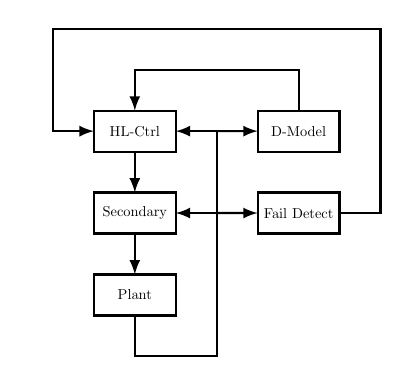
\begin{tikzpicture}[thick,scale=0.52, every node/.style={scale=0.52}]
\node (h) at (0,3) {HL-Ctrl};
\draw  (1,2.5) rectangle (-1,3.5);
\node (b) at (0,1) {Secondary};
\node  (t) at (0,-1) {Plant};
\draw  (1,0.5) rectangle (-1,1.5);
\draw  (1,-1.5) rectangle (-1,-0.5);
\draw (-2.5,-2);
\node at (4,3) {D-Model};
\node at (4,1) {Fail Detect};
\draw  (3,3.5) rectangle (5,2.5);
\draw  (3,1.5) rectangle (5,0.5);
\draw [-latex](0,2.5) -- (0,1.5);
\draw [-latex](0,0.5) -- (0,-0.5);
\draw [-latex](0,-1.5) -- (0,-2.5) -- (2,-2.5) -- (2,3) coordinate (v2) {} -- (1,3);
\draw [-latex](2,1) coordinate (v1) {} -- (1,1);
\draw [-latex](v1) -- (3,1);
\draw [-latex](v2) -- (3,3);
\draw [-latex](4,3.5) -- (4,4.5) -- (0,4.5) -- (0,3.5);
\draw [-latex](5,1) -- (6,1) -- (6,5.5) -- (-2,5.5) -- (-2,3) -- (-1,3);
\node at (-2.5,2) {};
\end{tikzpicture}
        \caption{A simplified view of how the controllers and sensing tie together} \label{fig:schematic}
\end{figure}

\begin{description}
        \item[The High-Level Controller] (HL-Ctrl) would dictate how each component (Electrolyser, SOFC and Gas Turbine) would be used, given information on failure states, predicted future demand, and the current system state. This is explored in Sections \ref{sec:power-pid} and \ref{sec:lqr}.
        \item[The Secondary Controller] would be a Virtual Inertia, a method used to simulate a large grid inertia with more inexpensive methods. {This is explored in Section \ref{sec:vi}, \emph{but not in depth.}}
        \item[Failure detection] can be achieved via a Kalman filter as suggested by \cite{power:kalman}, and the information gained can inform the controller of possible constraints. {This is mentioned in Section \ref{sec:failurestate}.}
        \item[A Disturbance Model] can aid in the case of MPC, future disturbance is \emph{not known} in a causal system. By having a disturbance model, the system can predict (using a Markov Chain \cite{power:markovP}) what the future state will be.
        \item[The `Plant' block] is where most of the design effort was focused, forming a model of the power-production and material balance will help greatly in deciding if this is a viable method of energy storage. {This is explored below in moderate depth, using device parameters from Section \ref{sec:sysdyn} to be implemented in Section \ref{sec:plant}.}
\end{description}

This topology would be ideal as the High-Level controller would dictate the control of the plant for the most cost-effective response.
The Secondary (Virtual Inertia) controller would manage very fast changes in the system state - to ensure a low enough bandwidth for any High-Level controller operation.
The High-Level controller would require state information from the disturbance model on future demand predictions, as well as the actual plant state (component actuation, grid frequency).
Failure detection would be important in later iterations to guarantee the plant runs safely in all possible conditions - to ensure a stable electricity supply for consumers.

\subsubsection{Process of Implementation}

Implementation began by designing the core components of the plant.
Approximate models for each component were formed.
This allowed observations of responses to step requests, and from there constructed simple methods of control.
Proportional, PID and LQR schemes were explored to check stability and find the optimal result.
LQR was implemented, and model complexity was added.

Alongside development of the plant and classical controllers, methods on disturbance modelling were explored and data were collected to aid with the exploration piece of Model Predictive Control.

\subsection{LQR Problem Formulation}

\subsubsection{State Space System}
\label{sec:lqr}

The design begin by considering the system as a \emph{State Space}, this takes into account {\color{red}system dynamics}, {\color{blue}input effects}, and predicted {\color{green}disturbance effects}. This model used the data generated from Table \ref{tbl:powercomp}, and uses the system state $\vv{\bm{x}}$ to construct a model.

    \begin{equation}
            {\color{red} \frac{ \partial \vv{\bm{x}} }{ \partial t } }  = {\color{red} \bm{A} \vv{\bm{x}}} + {\color{blue}\bm{B}{\bm{u}} }+ {\color{green}\bm{D} d}
    \end{equation}
        \begin{equation}
            y = \bm{C} \vv{\bm{x}}
        \end{equation}
        \begin{equation}
                \vv{\bm{x}} =
                \begin{bmatrix}
                        e_{\omega}\\
                        T_{t}\\
                        T_{s}\\
                        T_{e}\\
                \end{bmatrix}
                ,
                \qquad
                \bm{u} =
                \begin{bmatrix}
                        u_t\\
                        u_s\\
                        u_e\\
                \end{bmatrix}
                ,
                \qquad
                \bm{d} =
                \begin{bmatrix}
                        d_{\text{demand}}\\
                        d_{\text{cryostill}}\\
                        d_{\text{wind}}
                \end{bmatrix}
                ,
                \qquad
                \bm{D} =
                \begin{bmatrix}
                        -1 & -1 & 1 \\
                        %\multicolumn{2}{c}{\smash{\raisebox{0\normalbaselineskip}{$ \bm{0}_{4,3}$}}}\\
                        \, & \bm{0}_{4,3} & \, \\
                \end{bmatrix}
        \end{equation}
        \begin{equation}
                \bm{A} =
                \begin{bmatrix}
                        0 & J^{-1}& J^{-1}& -J^{-1}\\
                        0 & -k_t & 0 & 0\\
                        0 & 0 & -k_s & 0\\
                        0 & 0 & 0 & -k_e
                \end{bmatrix}
                , \qquad \bm{B} =
                \begin{bmatrix}
                        0 & 0 & 0 \\
                        -k_t & 0 & 0\\
                        0 & -k_s & 0\\
                        0 & 0 & -k_e
                \end{bmatrix}
        \end{equation}



%    \begin{equation}
%            {\color{red} \frac{ \partial \vv{\bm{x}} }{ \partial t } }  = {\color{red} \bm{A} \vv{\bm{x}}} + {\color{blue}\bm{B}{\bm{u}} }+ {\color{green}\bm{D} d}
%    \end{equation}
%        \begin{equation}
%            y = \bm{C} \vv{\bm{x}}
%        \end{equation}
%        \begin{equation}
%                \vv{\bm{x}} =
%                \begin{bmatrix}
%                        e_{\omega}\\
%                        T_{t}\\
%                        T_{s}\\
%                        T_{e}\\
%                        T_{b}\\
%                \end{bmatrix}
%                ,
%                \qquad
%                \bm{u} =
%                \begin{bmatrix}
%                        u_t\\
%                        u_s\\
%                        u_e\\
%                        u_b\\
%                \end{bmatrix}
%                ,
%                \qquad
%                \bm{d} =
%                \begin{bmatrix}
%                        d_{\text{demand}}\\
%                        d_{\text{cryostill}}\\
%                        d_{\text{wind}}
%                \end{bmatrix}
%                ,
%                \qquad
%                \bm{D} =
%                \begin{bmatrix}
%                        -1 & -1 & 1 \\
%                        %\multicolumn{2}{c}{\smash{\raisebox{0\normalbaselineskip}{$ \bm{0}_{4,3}$}}}\\
%                        \, & \bm{0}_{4,3} & \, \\
%                \end{bmatrix}
%        \end{equation}
%\begin{equation}
%                \bm{A} =
%                \begin{bmatrix}
%                        0 & 60\J^{-1}& 60J^{-1}& -60J^{-1}& -60J^{-1}\\
%                        0 & -k_t & 0 & 0 & 0\\
%                        0 & 0 & -k_s & 0 & 0\\
%                        0 & 0 & 0 & -k_e & 0\\
%                        0 & 0 & 0 & 0 & -k_b\\
%                \end{bmatrix}
%                , \qquad \bm{B} =
%                \begin{bmatrix}
%                        0 & 0 & 0 & 0\\
%                        -k_t & 0 & 0 & 0\\
%                        0 & -k_s & 0 & 0\\
%                        0 & 0 & -k_e & 0\\
%                        0 & 0 & 0 & -k_b\\
%                \end{bmatrix}
%        \end{equation}
%

For this \emph{State Space}, the angular frequency error term $\qquad e_{\omega} = \omega_{g} - \omega_{g0}$ was used, and loads were modelled by time-varying disturbance terms $d_i$.

\emph{Noiseless full-state feedback} was assumed, as it is known can observe each property individually, and known methods on noise rejection exist.
Should a state not be observable, an \emph{observer} can be constructed to predict that state. \cite{power:controlman}

\subsubsection{Augmented Integrator State}

To obtain integral action from the LQR, an `augmented' state can be created, which is the integral of the error state measured \cite{power:augstate}. This is executed through creating an augmented system:

    \begin{equation}
            \frac{ \partial \vv{\bm{x_a}} }{ \partial t }   =  \bm{A_a} \vv{\bm{x_a}} + \bm{B_a}{\bm{u}} + \bm{D_a} \bm{d}
    \end{equation}
    Such that:
    \begin{equation}
            \vv{\bm{x_a}} = 
            \begin{bmatrix}
                    I_{\omega}\\
                    \vv{\bm{x}}
            \end{bmatrix}
        , \qquad
            \bm{A_a} = 
            \begin{bmatrix}
                    0 & 1 & 0 & 0 & 0 & 0\\
                 \multicolumn{6}{c}{\smash{\raisebox{0\normalbaselineskip}{$ \bm{A} $}}}\\
            \end{bmatrix}
        , \qquad
            \bm{B_a} = 
            \begin{bmatrix}
                    \bm{0}_{1,4}\\
                    \bm{B}
            \end{bmatrix}
        , \qquad
            \bm{D_a} = 
            \begin{bmatrix}
                    \bm{0}_{1,3}\\
                    \bm{D}
            \end{bmatrix}
    \end{equation}

This was repeated for an additional integral state, giving double integral (or gradient tracking) action.


\subsubsection{Cost Function Structure}

Producing the optimal LQR controller involves minimising the cost function $J^{\prime}$: 
\begin{equation}
        J^{\prime} = \int^{\infty}_{0} (\, \vv{\bm{x}}^{\mathrm{T}} \bm{Q} \vv{\bm{x}} + \bm{u}^{\mathrm{T}} \bm{R} \bm{u} \,) \, \dd t
\end{equation}
Such that with feedback  $\bm{u} = -\bm{G} \vv{\bm{x}}$ an obtain optimal state feedback matrix $\bm{G}$ can be obtained.
MATLAB conveniently has the built-in function \code{\color{blue}lqr}, which takes as arguments the weighting matrices $\bm{Q}$ and $\bm{R}$ and returns the gain matrix $\bm{G}$.

As an aside, \code{\color{blue}lqr} works as a \emph{known solution} to the above cost function is $\bm{G} = \bm{R}^{-1} ( \bm{B}^T \bm{P})$, where $\bm{P}$ is found from solving the Algebraic Riccati Equation: $\bm{A}^T \bm{P} + \bm{P}\bm{A} - \bm{P}\bm{B}\bm{R}^{-1}\bm{B}^T\bm{P} = 0$. \cite{power:controlman}

This can be applied to a regular LQR and the LQR with augmented state, such that multi-state P and PI control can be achieved.

\subsubsection{Parallel LQR with Augmented State}

By using the same argument as in Section \ref{sec:power-pid}, the SOFC should manage all disturbance that it plausibly can without turbine intervention - just for the argument that the SOFC will use less ammonia and therefore reduce plant size.
The SOFC therefore has to have integral action to reject DC error (as integrators have infinite gain at DC).
The SOFC will also have a high gain, or a low cost associated with it.
After some experimentation it was found that double integral action on the SOFC increased performance and reduced low frequency oscillations on high frequency load changes.

Turbine intervention is for large proportional error, so integral action is not desired.
Turbine control also had higher cost associated with it, such that the SOFC is preferred if possible.

Overall the frequency error \emph{must be inside tolerances} (recall Section \ref{sec:pwrintro}), therefore cost associated with frequency error is the highest, with the integral terms tuned for best response.


\subsubsection{Non-Idealities and Assumptions}

In this analysis all components are assumed as first order, linear, have no time delay, and have the ability to supply positive and negative power.
In reality the SOFC and Turbine can only give power to the grid, and the electrolyser can only take power from the grid, so the LQR method \emph{will not be ideal}.

A parallel combination of the LQR and augmented-state LQR may also not be ideal - since some feedback terms are rejected, and each system is unaware of the other.

Inputs are also limited such that $ 0 \leq u \leq 1$, which is another non-ideality.
With gains too high (input costs too low), control becomes bang-bang may lose the ability to finely regulate the system.
Another consequence of my assumptions is that the plant can satisfy all demand put on it with zero error at DC.

Turbines have a cost associated with starting up - the amount of wear in a turbine (what defines the time between services) is determined by the number of spin-up events.
The blades in the turbine undergo one stress cycle when the engine spools up to speed which (by Miners Rule) determines the damage undertaken by the engine.
Preventing unnecessary start-ups can be achieved by a threshold, which introduces \emph{another non-ideality} into the system.
Another non-ideality on the system is the limits on the integrator.
Limits were imposed to prevent windup, and these were tuned for performance.
Results from the implementation are analysed below in Section \ref{sec:pwrtesting}.

\subsection{MPC Problem Formulation}
\subsubsection{Conversion of State Space to MPC}
\label{sec:mpc}

To convert from continuous time to discrete time, the \emph{State Space} was transformed (as suggested by \cite{power:mpcform}):

Firstly by recalling the original State Space:
\begin{equation}
        \frac{\partial \vv{\bm{x}}}{\partial t} = \bm{A} \vv{\bm{x}} + \bm{B} \bm{u} + \bm{D} \bm{d}
\end{equation}
Discretise - $t_k = kT_s$ where $T_s$ is the sample time:
\begin{equation}
        \bm{x}(t_{k+1}) = \bm{A}^{\prime} \bm{x}(t_k) + \bm{B}^{\prime}\bm{u}(t_k) + \bm{D}^{\prime}\bm{d}(t_k)
\end{equation}
Where discretisation is performed by:
\begin{equation}
        \bm{A}^{\prime} \equiv \mathrm{e}^{\bm{A}T_s}
        , \qquad \bm{B}^{\prime} \equiv \int^{T_s}_0\mathrm{e}^{\bm{A} \eta} \bm{B} \mathrm{d} \eta ,
        \qquad \bm{D}^{\prime} \equiv \int^{T_s}_0\mathrm{e}^{\bm{A} \eta} \bm{D} \mathrm{d} \eta
\end{equation}
{\color{red}To Be Continued.. Maybe Remove this Section.}

MATLAB has a built in funciton that does this transformation, \code{c2d} which was used to convert to discrete time-based systems.

\subsubsection{Constraints for the MPC}
Lorem Ipsum



\subsection{Disturbance Modelling for MPC}
\label{sec:markov}

The disturbance that was of most interest is the load from consumers on the grid.
The assumption that the load disturbance is modelled as a deterministic process is reasonable. 
The load-cycles on the grid are periodic, and therefore it seems reasonable to suggest a machine could predict what a future demand will be.
Hawaii has a very small change in climate throughout the year - from 20 to 25 degrees Celsius, meaning there is not a large change in load between winter and summer months.

A decision was made that a suitable object to model electrical loads was a Markov Chain - as it takes into account differing patterns in demand.
This object allows for interesting behaviour, for example if the grid is on a path that looks like a weekend demand curve, the Markov Chain will more likely predict demands characteristic of weekends.
The Markov Chain has proved reliable in these situations \cite{power:markovP} which is what allowed this decision.

\textbf{What is a Markov Chain?}
A stochastic model that describes a sequence of state changes, in which the probability of the next state change, depends \emph{only} on the state obtained from the previous change.

\subsubsection{Normalizing Data}

Consumers are becoming more and more dependant on electrical power, in the United States alone, power consumption \emph{per household} was only 10,000 kWh per anum, yet in 2010, power consumption was 11,500 kWh per anum \cite{power:growth}.

To find a way of normalizing the power demand data-set - such that more, old data can be used to build the stochastic matrix, a scaling factor that varies with time must be considered.
The scaling factor used is $\zeta(t^{\prime})$, where $t^{\prime}$ is the days since 1/1/2000.

It was assumed $\zeta$ has form:
\begin{equation}
        \zeta(t^{\prime}) = a t^{\prime} + b
\end{equation}
To find coefficients $a$ and $b$, $\max P$ was plotted for each week, and use a Huber regression.

It was found that $a = 202$, $b = 1.97$.

\subsubsection{Markov Chain Formulation}

To start the formulation, power demand was discretised into a array $F$ of size $N$.

If the demand is known to be $\zeta(t^{\prime}) F(i)$ at time $Tk$, then the probability of demand being $F(j)$ at time $T(k+1)$ is represented by the location in a matrix: $M_{i,j,k}$.
The expectation of demand at time $k+1$ is $\sum^{N}_{j=0} \zeta(t^{\prime}) F(j) M_{i,j,k}$. 

The data is discretised into 10 minute time-slices and form the 3-D stochastic matrix from it.

\begin{figure}[bht]
        \centering
\usetikzlibrary{arrows}
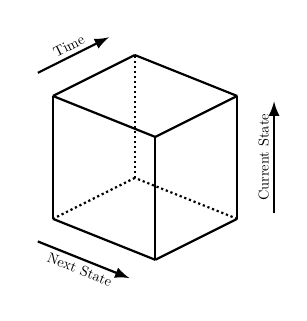
\begin{tikzpicture}[thick,scale=0.52, every node/.style={scale=0.52}]
\coordinate (v1) at (-2,-1.5) {};
\coordinate (v7) at (0,-0.5) {};
\coordinate (v6) at (0.5,-2.5) {};
\coordinate (v5) at (2.5,-1.5) {};
\coordinate (v2) at (-2,-4.5) {};
\coordinate (v3) at (0.5,-5.5) {};
\coordinate (v4) at (2.5,-4.5) {};
\coordinate (v8) at (0,-3.5) {};
\draw  (v1) edge (v2);
\draw  (v2) edge (v3);
\draw  (v3) edge (v4);
\draw  (v5) edge (v4);
\draw  (v6) edge (v5);
\draw  (v1) edge (v6);
\draw  (v1) edge (v7);
\draw  (v7) edge (v5);
\draw  (v6) edge (v3);
\draw [densely dotted] (v4) edge (v8);
\draw [densely dotted] (v8) edge (v2);
\draw [densely dotted] (v8) edge (v7);
\node (v11) at (-2.5,-1) {};
\node (v12) at (-0.5,0) {};
\node (v13) at (-2.5,-5) {};
\node (v14) at (0,-6) {};
\node (v9) at (3.4,-4.5) {};
\node (v10) at (3.4,-1.5) {};\tikzstyle{myedgestyle} = [-latex]
        \draw [-latex] (v11) edge node[sloped, anchor=center, above] {Time} (v12);
        \draw [-latex] (v13) edge node[sloped, anchor=center, below] {Next State} (v14);
        \draw [-latex] (v9) edge node[sloped, anchor=center, above] {Current State} (v10);
\end{tikzpicture}
        \caption{A simplified view of what the stochastic matrix, $M$ will look like.} \label{fig:markov}
\end{figure}
For each day, $k=0$ was set at midnight.
Then to the following for each day of data:

By considering time $k$ (which sets which layer to edit), the $i$ state the system is in is known (which row on the stochastic matrix is being edited).
The state for time $k+1$, which shall be called $i^\prime$ is observed and passed to the next step.
Knowing $i$, $j = i^\prime$, and $k$ - location $M_{i,i^\prime,k}$ is incremented by one.

At this stage a matrix that documents all the state transitions exists - where states were from and where they were to at discrete times.
Only 5 years ($\approx 1800$ days) of data is available, however if the contents of a single row are plotted, Gaussian-like behaviour was observed.
Most probability distributions tend towards the Gaussian for large $n$, this is known as the Central Limit Theorem.

By assuming statistics for state transition is Gaussian in behaviour, it is possible under \emph{Maximum Likelihood Estimation} to estimate centroid location, as well as variance and fit a Gaussian to it.
This hopefully more accurately captures the dynamics of the real system, given the dataset used was not large.

\subsubsection{Obtaining a Disturbance Prediction}

A simple algorithm was developed that takes a walk through the matrix.
The probability of state change is defined by the stochastic matrix, this was used by the algorithm to walk through the data set and generate a predicted load pattern.
By running many (on the order of 10000) runs through the data, the mean path is calculated which is the predicted disturbance.

\subsection{Controller and Plant Testing}
\label{sec:pwrtesting}

{\bf \color{red} This section is not finished - I need to finish my analysis.}
\subsubsection{Plant Tests}

Step responses were observed for the components, these conformed to expectations and the test was deemed successful.
{\color{red}Step Response Figures Here}

Tanks were tested and operated as expected.


\subsubsection{Plant with a PID/PD Combination}

I found that the system was able to give a good response.
Response was not optimal, and there were issues with the Electrolyser {\color{red}(comment more)}

\subsubsection{Plant with LQR Controller}

\subsubsection{Plant with a Augmented LQR Combination}
\begin{figure}[htp]
\centering
\includegraphics[width=.33\textwidth]{images/sim/sim1_disturb.eps}\hfill
\includegraphics[width=.33\textwidth]{images/sim/sim1_omega.eps}\hfill
\includegraphics[width=.33\textwidth]{images/sim/sim1_util.eps}
        \caption{Simulation Run for LQR Controller with Augmented States, under \emph{Very Harsh} Conditions To Demonstrate Controller Robustness.}
        \label{fig:sim1}
\end{figure}
System was able to perform well under simulated harsh conditions, with minimal frequency error under a low inertia state.

Compared to PID I observed step responses are {\color{red}XXXX}.
%%todo make this better

\begin{itemize}
{\color{red}
\item We need to model errors in the system we predict
\item We need to model errors in efficiency assumptions - check with less efficient systems
\item We need to model errors in disturbance prediction - see above
}
\end{itemize}

\subsection{Secondary Controller - Virtual Inertia}
\label{sec:vi}

\subsubsection{Reason For Implementation}

As discussed through this section, electrical grids require an `inertial component' to reduce the bandwidth and aid in achieving stability of the system.
Another way of looking at inertia is as a stored energy in the rotating generation units, this interpretation can be used in making an active, inexpensive inertia for the grid.

Implementing real inertia is expensive, as it requires the investment of the mass that will be rotating synchronously with the grid as well as the means of coupling the large inertia to the grid.

Especially problematic are the Wind Turbines and SOFCs, as they produce a DC current which is inverted to make AC for transmission.
The power inverter is a switch mode system that has a small inertia, so an active method for increasing inertia is required.

\subsubsection{Specification for Implementation}

A control system with a battery-bank can be used to feed power into the grid.
Batteries are DC units, whereas the grid is AC so an inverter is needed as well.

By re-using Equation \ref{swing} it is possible to make a control system that acts as a virtual inertia on the grid \cite{power:inertia}.
Solutions exist \cite{power:inertia} that introduce a virtual inertia to the electrical grid. 

The inertia used on the simulation found to give a compromise between fast response and tracking performance was $80 \cdot 10^3\text{kgm}^2$, which would be used to define the scale of the virtual inertia.

\subsection{Operation in Fail-States}
\label{sec:failurestate}

When a fault is detected, the component would be taken offline.
This removes it from the generated State Space, and means the controller has to adapt to stabilise the dynamics of the plant.

Should a generation-side component fail, the grid is at risk of not having enough energy and frequency dropping to dangerous levels.
For this reason, the SOFCs and Turbine are paralleised, such that a single turbine \emph{can be taken offline}, as more are able to step in and ensure operation.

Should all of one type of generation-side component fail, for example the SOFC, the turbine will have to make up all the load deficit.
The turbine was not designed to have integral action, so there will be a proportional frequency error if another controller doesn't introduce integral action.
Therefore failure detection should be used (through a Kalman filter as suggested by \cite{power:kalman}) which will trigger the action of an integrator on the turbine.

Should a single electrolyser fail the remainder of active cells will consume the required amount of energy to sustain correct frequency.
Should all the electrolyser units fail, the plant will have to dump power from the grid to prevent the frequency rising and damaging domestic equipment.
This can be achieved by a \emph{load bank} which is nothing more than an array of actively cooled resistors.
Such systems are avaliable for purchase and an example found can continuously dissapate 1MW \cite{power:rdump}.

Since simulations found a maximum net power on the grid of 250MW, 300 such resistive load dumps would be needed (safey factor of 1.2). 
The control signal from the electrolyser can be redirected to the load dumps, as they have a comparable response time.

Should a catastrophic failure occur causing the plant to not keep up with demand, \emph{load shedding} will happen, which is a protective method to keep some of the grid alive and prevent a \emph{black start}. This is discussed in more detail in section \ref{sec:challengespwr}.

\subsection{Risks and Challenges}

\subsubsection{Solar Power}

Solar panel adoption in the United States is increasing year-upon-year, which (depending on solar isolation) can cause `back-feed' events occurring like in Figure \ref{fig:solar}.
An Energy Storage System would benefit in this case as the energy back-fed can be stored for later usage, in a similar way to how the wind turbines perform.
The challenge associated with this model is that since wind and load effects were considered, the MPC's disturbance prediction would have to incorporate the power supplied by solar panels as well, to ensure accurate control.
As visible on the Figure \ref{fig:solar}, this is changing significantly every year, so more research would be required for this case.
Another implication is that fewer wind turbines would be required, and the plant may end up generating excess Hydrogen and Ammonia.
\begin{figure}[htb]
\includegraphics[scale=0.3]{images/backfeed.jpg}
\caption{The Effect of Increased Solar Adoption \cite{power:solar}}
\label{fig:solar}
\end{figure}

\subsubsection{Modelling Errors}

The model developed in Section \ref{sec:plant} is by no means a fully-accurate model of the plant.
More work will have to be done in constructing deep models of each component for the removal of the bulk of the errors.
Some other, not fully explored errors also include:
Demand data was also approximated with cubic splines to give higher resolution data for simulation.
Wind speed was approximated with cubic splines so better data at a higher resolution are required to form a more accurate model.
Wind turbine dynamics were approximated as steady state for all wind speeds and the coupling to the grid was assumed to be perfect.
A better understanding on how components couple to the electrical grid is crucial for this project to be better understood and more accurate.

\subsubsection{Grid Black-start}
\label{sec:challengespwr}

Should an event occur that knocks the grid offline, a \emph{black-start} will be required.
This is challenging as the full 230MW grid load will be drawing power at the same time, and the act of switching on the power is a step request (which acts at a high bandwidth).
Black-starts therefore take on the order of days to execute, in the UK the Restoration Time for 60\% of the grid's demand is 24 hours \cite{power:natgridblack}.
A protocol would have to be written to deal with this rare but not-impossible risk, to ensure a fast recovery from disaster.

\subsection{Plant Scaling}
\label{sec:plantscale}

Plant scaling is a rather important section as it dictats the flowrates and storage requirements the plant has to adhere to, in order to satisfy consumer demand.

The plant simulation was used with demand and wind data fed into the function blocks (see Figure \ref{fig:global}). A simulation was run to obtain an estimate on the material and energy requirements for the plant.

The material balance for the first design iteration was produced in Figure \ref{flowsheettbl}.

These data were used to scale other components and to demonstrate that with approximate efficiency values from literature that this is a feasible project (see sections \ref{} and \ref{}).

A rather startling conclusion from this analysis is that the ESS stores far less energy than was orginally expected.
The windspeeds in Maui are sufficiently high all-year-round to satisfy the bulk of consumer demand.

\begin{figure}[tbh]
    \centering
    \includegraphics[scale=0.9]{images/flowtable.pdf}
    \caption{An approximate material balance flowsheet using efficiency factors from all components, demand and wind data.}
    \label{flowsheettbl}
\end{figure}
\subsection{Conclusion}

This section on power control and plant simulation was overall successful.
The simulation proved useful in obtaining scaling figures for the plant, which were used in other sections, as well as validating the control scheme designed.

The controller survived far harsher conditions than those in reality, so robustness has been tested and the control scheme validated for the simplified case.
In the case of real data applied the system, the maximum frequency error delta is no more than $4 \text{rads}^-1$ which is within desired bounds.
The material flows were validated to show the plant's scale is correct to a first order approximation, and the plant is in fact viable for this location.

\begin{thebibliography}{9}
%\bibitem{power:freqs}
%Frequency Control Concerns In The North American Electric Power System
%\textbf{Consortium for Electric Reliability Technology Solutions}
%\url{https://info.ornl.gov/sites/publications/Files/Pub57419.pdf}

%\bibitem{power:mpcadvs}
%Process Control in the Chemical Industries
%Model Predictive Control - An Introduction (2002)
%Chemical Engineering Department,
King Saud University

%\bibitem{power:timecorrection}
%Impacts of Power Grid Frequency Deviation on Time Error of Synchronous Electric Clock and Worldwide Power System Practices on Time Error Correction

%\bibitem{power:swing}
 %Grainger, John J.; Stevenson, William D. (1 January 1994). Power system analysis. McGraw-Hill. ISBN 978-0-07-061293-8.

%\bibitem{power:vi}
%Impact of Low Rotational Inertia on
%Power System Stability and Operation
%Andreas Ulbig, Theodor S. Borsche and Göran Andersson Power Systems Laboratory, ETH Zurich
%22 Dec 14

%\bibitem{power:wturbine}
%A Critical Review on Wind Turbine Power Curve Modelling Techniques and Their Applications in Wind Based Energy Systems
%Vaishali Sohoni, S. C. Gupta, and R. K. Nema
%Journal of Energy
%Volume 2016 (2016), Article ID 8519785, 18 pages

%\bibitem{power:wturbdata}
%GE Haliade Datasheet
%\url{http://offshorewind.net/wp-content/uploads/2016/01/Haliade-150-6MW-offshore-wind-turbine.pdf}

\bibitem{power:NOAA}
NOAA WEBSITE WHERE I GOT MY DATA

%\bibitem{power:kalman}
%Adaptive Kalman filtering, failure detection and identification for spacecraft attitude estimation
%R. Mehra, S. Seereeram, D. Bayard, F. Hadaegh
%1995

%\bibitem{power:controlman}
%Kwakernaak, Huibert & Sivan, Raphael (1972). Linear Optimal Control Systems. First Edition. Wiley-Interscience. ISBN 0-471-51110-2.

%state augmentation
%\bibitem{power:augstate}
%Comparison of Two Methods of Incorporating an Integral Action in Linear Quadratic Regulator
%Hanmant G. Malkapure. M. Chidambarami, Indian Institute of Technology Madras, Chennai
%Department of Chemical Engineering
%2014

%mpc
%\bibitem{power:mpcform}
%Model Predictive Control of Continuous-Time Nonlinear Systems With Piecewise Constant Control.
%Mangi. L, Scattolini, R.
%IEEE Transactions on Automatic Control, Vol49, %No 6, June 2004



%\bibitem{power:markovP}
%Markovian Models for Electrical Load Prediction in Smart Buildings
%M. K. Haider, A. K. Ismail, I. A. Qazi
%\url{http://web.lums.edu.pk/~ihsan/papers/ICONIP-2012.pdf}
Last Accessed 1/2/2018

%Disturbance Modeling
%\bibitem{power:growth}
%Growth of US power consumption

%virtual inertia
%\bibitem{power:inertia}
%Grid Inertial Response with Lithium-ion Battery Energy Storage Systems
%Knap. V, Sinha. R
%\url{http://projekter.aau.dk/projekter/files/77175981/master.pdf}
Last Accessed 10/2/2018

%\bibitem{power:rdump}
%Datasheet for Resistive Load Dump
%https://www.comrent.com/wp-content/uploads/2016/11/MS110-1000kw.pdf
%Last Accessed 1/2/2018
                
\bibitem{power:natgridblack}
Black Start Strategy, National Grid.
August 2017
\url{https://www.nationalgrid.com/sites/default/files/documents/High%20Level%20Black%20Start%20Strategy.pdf}
Last Accessed 1/2/2018

\end{thebibliography}


%\end{document}

\end{document}